\documentclass{book}
\usepackage[a4paper,top=2.5cm,bottom=2.5cm,left=2.5cm,right=2.5cm]{geometry}
\usepackage{makeidx}
\usepackage{natbib}
\usepackage{graphicx}
\usepackage{multicol}
\usepackage{float}
\usepackage{listings}
\usepackage{color}
\usepackage{ifthen}
\usepackage[table]{xcolor}
\usepackage{textcomp}
\usepackage{alltt}
\usepackage[utf8]{inputenc}
\usepackage{mathptmx}
\usepackage[scaled=.90]{helvet}
\usepackage{courier}
\usepackage{sectsty}
\usepackage[titles]{tocloft}
\usepackage{doxygen}
\lstset{language=C++,inputencoding=utf8,basicstyle=\footnotesize,breaklines=true,breakatwhitespace=true,tabsize=8,numbers=left }
\makeindex
\setcounter{tocdepth}{3}
\renewcommand{\footrulewidth}{0.4pt}
\renewcommand{\familydefault}{\sfdefault}
\hfuzz=15pt
\setlength{\emergencystretch}{15pt}
\hbadness=750
\tolerance=750
\begin{document}
\begin{titlepage}
\vspace*{7cm}
\begin{center}
{\Large L\-O21\-\_\-final\-\_\-diallo\-\_\-lu }\\
\vspace*{1cm}
{\large Generated by Doxygen 1.8.1.1}\\
\vspace*{0.5cm}
{\small Thu Jun 21 2012 15:12:57}\\
\end{center}
\end{titlepage}
\clearemptydoublepage
\pagenumbering{roman}
\tableofcontents
\clearemptydoublepage
\pagenumbering{arabic}
\chapter{Namespace Index}
\section{Namespace List}
Here is a list of all namespaces with brief descriptions\-:\begin{DoxyCompactList}
\item\contentsline{section}{{\bf Ui} }{\pageref{namespace_ui}}{}
\end{DoxyCompactList}

\chapter{Class Index}
\section{Class Hierarchy}
This inheritance list is sorted roughly, but not completely, alphabetically\-:\begin{DoxyCompactList}
\item \contentsline{section}{Expression}{\pageref{class_expression}}{}
\begin{DoxyCompactList}
\item \contentsline{section}{Constant}{\pageref{class_constant}}{}
\item \contentsline{section}{Nombre}{\pageref{class_nombre}}{}
\begin{DoxyCompactList}
\item \contentsline{section}{Complexe}{\pageref{class_complexe}}{}
\item \contentsline{section}{Entier}{\pageref{class_entier}}{}
\item \contentsline{section}{Rationnel}{\pageref{class_rationnel}}{}
\item \contentsline{section}{Reel}{\pageref{class_reel}}{}
\end{DoxyCompactList}
\item \contentsline{section}{Operation}{\pageref{class_operation}}{}
\begin{DoxyCompactList}
\item \contentsline{section}{Operation\-Binaire}{\pageref{class_operation_binaire}}{}
\item \contentsline{section}{Operation\-Unaire}{\pageref{class_operation_unaire}}{}
\end{DoxyCompactList}
\end{DoxyCompactList}
\item \contentsline{section}{Main\-Window}{\pageref{class_main_window}}{}
\item \contentsline{section}{Pile}{\pageref{class_pile}}{}
\item \contentsline{section}{Ui\-\_\-\-Main\-Window}{\pageref{class_ui___main_window}}{}
\begin{DoxyCompactList}
\item \contentsline{section}{Ui\-:\-:Main\-Window}{\pageref{class_ui_1_1_main_window}}{}
\end{DoxyCompactList}
\end{DoxyCompactList}

\chapter{Class Index}
\section{Class List}
Here are the classes, structs, unions and interfaces with brief descriptions\-:\begin{DoxyCompactList}
\item\contentsline{section}{{\bf Complexe} }{\pageref{class_complexe}}{}
\item\contentsline{section}{{\bf Constant} }{\pageref{class_constant}}{}
\item\contentsline{section}{{\bf Entier} }{\pageref{class_entier}}{}
\item\contentsline{section}{{\bf Expression} }{\pageref{class_expression}}{}
\item\contentsline{section}{{\bf Ui\-::\-Main\-Window} }{\pageref{class_ui_1_1_main_window}}{}
\item\contentsline{section}{{\bf Main\-Window} }{\pageref{class_main_window}}{}
\item\contentsline{section}{{\bf Nombre} }{\pageref{class_nombre}}{}
\item\contentsline{section}{{\bf Operation} }{\pageref{class_operation}}{}
\item\contentsline{section}{{\bf Operation\-Binaire} }{\pageref{class_operation_binaire}}{}
\item\contentsline{section}{{\bf Operation\-Unaire} }{\pageref{class_operation_unaire}}{}
\item\contentsline{section}{{\bf Pile} }{\pageref{class_pile}}{}
\item\contentsline{section}{{\bf Rationnel} }{\pageref{class_rationnel}}{}
\item\contentsline{section}{{\bf Reel} }{\pageref{class_reel}}{}
\item\contentsline{section}{{\bf Ui\-\_\-\-Main\-Window} }{\pageref{class_ui___main_window}}{}
\end{DoxyCompactList}

\chapter{File Index}
\section{File List}
Here is a list of all files with brief descriptions\-:\begin{DoxyCompactList}
\item\contentsline{section}{calculatrice/{\bf expression.\-cpp} }{\pageref{expression_8cpp}}{}
\item\contentsline{section}{calculatrice/{\bf expression.\-h} }{\pageref{expression_8h}}{}
\item\contentsline{section}{calculatrice/{\bf main.\-cpp} }{\pageref{main_8cpp}}{}
\item\contentsline{section}{calculatrice/{\bf mainwindow.\-cpp} }{\pageref{mainwindow_8cpp}}{}
\item\contentsline{section}{calculatrice/{\bf mainwindow.\-h} }{\pageref{mainwindow_8h}}{}
\item\contentsline{section}{calculatrice/{\bf pile.\-cpp} }{\pageref{pile_8cpp}}{}
\item\contentsline{section}{calculatrice/{\bf pile.\-h} }{\pageref{pile_8h}}{}
\item\contentsline{section}{calculatrice/{\bf ui\-\_\-mainwindow.\-h} }{\pageref{ui__mainwindow_8h}}{}
\end{DoxyCompactList}

\chapter{Namespace Documentation}
\section{Ui Namespace Reference}
\label{namespace_ui}\index{Ui@{Ui}}
\subsection*{Classes}
\begin{DoxyCompactItemize}
\item 
class {\bf Main\-Window}
\end{DoxyCompactItemize}

\chapter{Class Documentation}
\section{Complexe Class Reference}
\label{class_complexe}\index{Complexe@{Complexe}}


{\ttfamily \#include $<$expression.\-h$>$}

Inheritance diagram for Complexe\-:\begin{figure}[H]
\begin{center}
\leavevmode
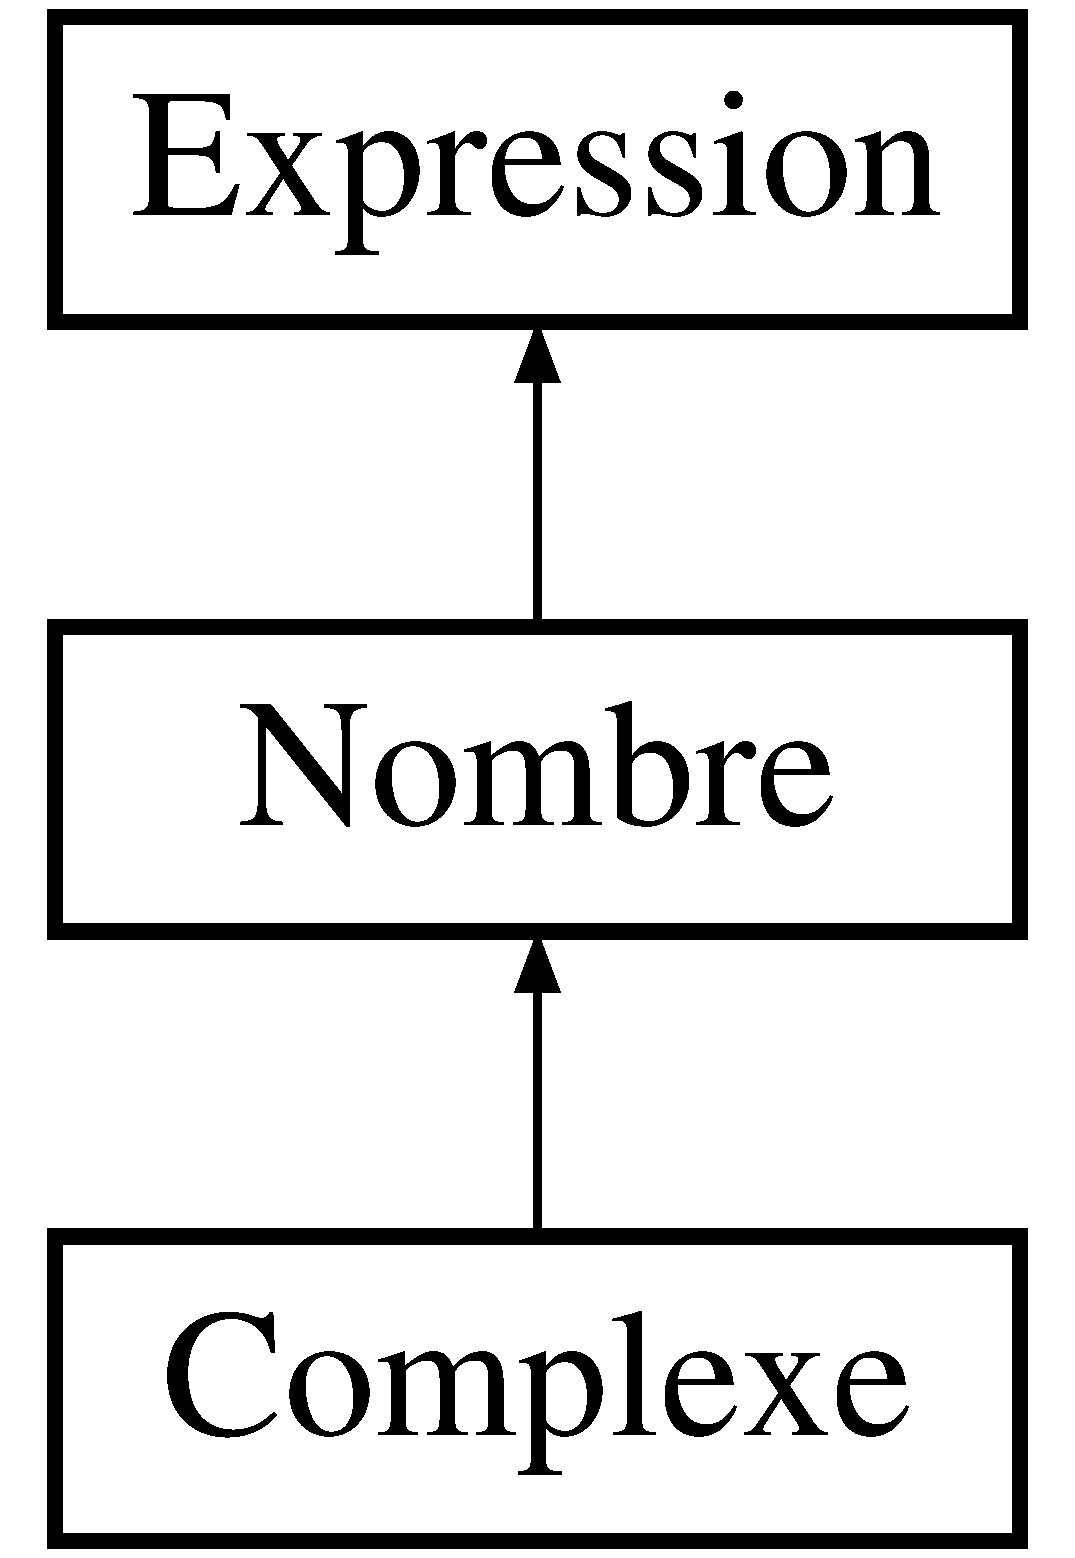
\includegraphics[height=3.000000cm]{class_complexe}
\end{center}
\end{figure}
\subsection*{Public Member Functions}
\begin{DoxyCompactItemize}
\item 
{\bf Complexe} (double partie\-Reelle, double partie\-Imaginaire)
\item 
{\bf Complexe} ({\bf Reel} \&r1, {\bf Reel} \&r2)
\item 
{\bf Complexe} ({\bf Rationnel} \&q1, {\bf Rationnel} \&q2)
\item 
{\bf Complexe} ({\bf Entier} \&e1, {\bf Entier} \&q2)
\item 
{\bf Complexe} ()
\item 
const {\bf Complexe} \& {\bf evaluer} () const 
\item 
Q\-String {\bf get\-Propriete} ()
\item 
{\bf Complexe} \& {\bf operator=} (const {\bf Complexe} \&c)
\item 
{\bf Nombre} \& {\bf operator+} (const {\bf Nombre} \&n)
\item 
{\bf Nombre} \& {\bf operator-\/} (const {\bf Nombre} \&n)
\item 
{\bf Nombre} \& {\bf operator$\ast$} (const {\bf Nombre} \&n)
\item 
{\bf Nombre} \& {\bf operator/} (const {\bf Nombre} \&n)
\end{DoxyCompactItemize}
\subsection*{Additional Inherited Members}


\subsection{Constructor \& Destructor Documentation}
\index{Complexe@{Complexe}!Complexe@{Complexe}}
\index{Complexe@{Complexe}!Complexe@{Complexe}}
\subsubsection[{Complexe}]{\setlength{\rightskip}{0pt plus 5cm}Complexe\-::\-Complexe (
\begin{DoxyParamCaption}
\item[{double}]{partie\-Reelle, }
\item[{double}]{partie\-Imaginaire}
\end{DoxyParamCaption}
)}\label{class_complexe_a0d199c9459ea8587ad0fe6f402420295}
\index{Complexe@{Complexe}!Complexe@{Complexe}}
\index{Complexe@{Complexe}!Complexe@{Complexe}}
\subsubsection[{Complexe}]{\setlength{\rightskip}{0pt plus 5cm}Complexe\-::\-Complexe (
\begin{DoxyParamCaption}
\item[{{\bf Reel} \&}]{r1, }
\item[{{\bf Reel} \&}]{r2}
\end{DoxyParamCaption}
)}\label{class_complexe_aaa287d52a7a4e3f2a4db5a84bf3b16de}
\index{Complexe@{Complexe}!Complexe@{Complexe}}
\index{Complexe@{Complexe}!Complexe@{Complexe}}
\subsubsection[{Complexe}]{\setlength{\rightskip}{0pt plus 5cm}Complexe\-::\-Complexe (
\begin{DoxyParamCaption}
\item[{{\bf Rationnel} \&}]{q1, }
\item[{{\bf Rationnel} \&}]{q2}
\end{DoxyParamCaption}
)}\label{class_complexe_a6be33361cfed41710e6ea42709ac5968}
\index{Complexe@{Complexe}!Complexe@{Complexe}}
\index{Complexe@{Complexe}!Complexe@{Complexe}}
\subsubsection[{Complexe}]{\setlength{\rightskip}{0pt plus 5cm}Complexe\-::\-Complexe (
\begin{DoxyParamCaption}
\item[{{\bf Entier} \&}]{e1, }
\item[{{\bf Entier} \&}]{q2}
\end{DoxyParamCaption}
)}\label{class_complexe_ad93280c51673fac403aa4db82c95ebfc}
\index{Complexe@{Complexe}!Complexe@{Complexe}}
\index{Complexe@{Complexe}!Complexe@{Complexe}}
\subsubsection[{Complexe}]{\setlength{\rightskip}{0pt plus 5cm}Complexe\-::\-Complexe (
\begin{DoxyParamCaption}
{}
\end{DoxyParamCaption}
)}\label{class_complexe_af2cec56db6fdf59ed5ec761ffd4e1608}


\subsection{Member Function Documentation}
\index{Complexe@{Complexe}!evaluer@{evaluer}}
\index{evaluer@{evaluer}!Complexe@{Complexe}}
\subsubsection[{evaluer}]{\setlength{\rightskip}{0pt plus 5cm}const {\bf Complexe} \& Complexe\-::evaluer (
\begin{DoxyParamCaption}
{}
\end{DoxyParamCaption}
) const\hspace{0.3cm}{\ttfamily [virtual]}}\label{class_complexe_a40c3fe088e4be07c905801596728ecce}


Implements {\bf Expression} \doxyref{}{p.}{class_expression_a883dfec27c4579cdd4749ce437d4925e}.

\index{Complexe@{Complexe}!get\-Propriete@{get\-Propriete}}
\index{get\-Propriete@{get\-Propriete}!Complexe@{Complexe}}
\subsubsection[{get\-Propriete}]{\setlength{\rightskip}{0pt plus 5cm}Q\-String Complexe\-::get\-Propriete (
\begin{DoxyParamCaption}
{}
\end{DoxyParamCaption}
)\hspace{0.3cm}{\ttfamily [inline]}, {\ttfamily [virtual]}}\label{class_complexe_a8cb62d7f0f5c0a1df7707362cd19d9b9}


Implements {\bf Expression} \doxyref{}{p.}{class_expression_a5c2940c8ca5195f5b9a51234c936e48c}.

\index{Complexe@{Complexe}!operator$\ast$@{operator$\ast$}}
\index{operator$\ast$@{operator$\ast$}!Complexe@{Complexe}}
\subsubsection[{operator$\ast$}]{\setlength{\rightskip}{0pt plus 5cm}{\bf Nombre} \& Complexe\-::operator$\ast$ (
\begin{DoxyParamCaption}
\item[{const {\bf Nombre} \&}]{n}
\end{DoxyParamCaption}
)\hspace{0.3cm}{\ttfamily [virtual]}}\label{class_complexe_a324a6de3198334550e8c704830ef4ce4}


Implements {\bf Nombre} \doxyref{}{p.}{class_nombre_ad249cd1678294bd419da8586ac9fbaa7}.

\index{Complexe@{Complexe}!operator+@{operator+}}
\index{operator+@{operator+}!Complexe@{Complexe}}
\subsubsection[{operator+}]{\setlength{\rightskip}{0pt plus 5cm}{\bf Nombre} \& Complexe\-::operator+ (
\begin{DoxyParamCaption}
\item[{const {\bf Nombre} \&}]{n}
\end{DoxyParamCaption}
)\hspace{0.3cm}{\ttfamily [virtual]}}\label{class_complexe_afb89aaf210d1f1b4ec021cff1a3e43a5}


Implements {\bf Nombre} \doxyref{}{p.}{class_nombre_a8672fd34bb479f72a9479c146cb33b48}.

\index{Complexe@{Complexe}!operator-\/@{operator-\/}}
\index{operator-\/@{operator-\/}!Complexe@{Complexe}}
\subsubsection[{operator-\/}]{\setlength{\rightskip}{0pt plus 5cm}{\bf Nombre} \& Complexe\-::operator-\/ (
\begin{DoxyParamCaption}
\item[{const {\bf Nombre} \&}]{n}
\end{DoxyParamCaption}
)\hspace{0.3cm}{\ttfamily [virtual]}}\label{class_complexe_af03cf172928fdd461f73ca90ad92826b}


Implements {\bf Nombre} \doxyref{}{p.}{class_nombre_a5a281bdf0efbc2a9b557abb8a58e8530}.

\index{Complexe@{Complexe}!operator/@{operator/}}
\index{operator/@{operator/}!Complexe@{Complexe}}
\subsubsection[{operator/}]{\setlength{\rightskip}{0pt plus 5cm}{\bf Nombre} \& Complexe\-::operator/ (
\begin{DoxyParamCaption}
\item[{const {\bf Nombre} \&}]{n}
\end{DoxyParamCaption}
)\hspace{0.3cm}{\ttfamily [virtual]}}\label{class_complexe_a5944d0f6628b7d8828ea5300dfe30a48}


Implements {\bf Nombre} \doxyref{}{p.}{class_nombre_a7b55aa0d106bbb34001161fe6e7b8ebc}.

\index{Complexe@{Complexe}!operator=@{operator=}}
\index{operator=@{operator=}!Complexe@{Complexe}}
\subsubsection[{operator=}]{\setlength{\rightskip}{0pt plus 5cm}{\bf Complexe} \& Complexe\-::operator= (
\begin{DoxyParamCaption}
\item[{const {\bf Complexe} \&}]{c}
\end{DoxyParamCaption}
)}\label{class_complexe_a31b944777f43db40b47e47c156aaa26c}


The documentation for this class was generated from the following files\-:\begin{DoxyCompactItemize}
\item 
calculatrice/{\bf expression.\-h}\item 
calculatrice/{\bf expression.\-cpp}\end{DoxyCompactItemize}

\section{Constant Class Reference}
\label{class_constant}\index{Constant@{Constant}}


{\ttfamily \#include $<$expression.\-h$>$}

Inheritance diagram for Constant\-:\begin{figure}[H]
\begin{center}
\leavevmode
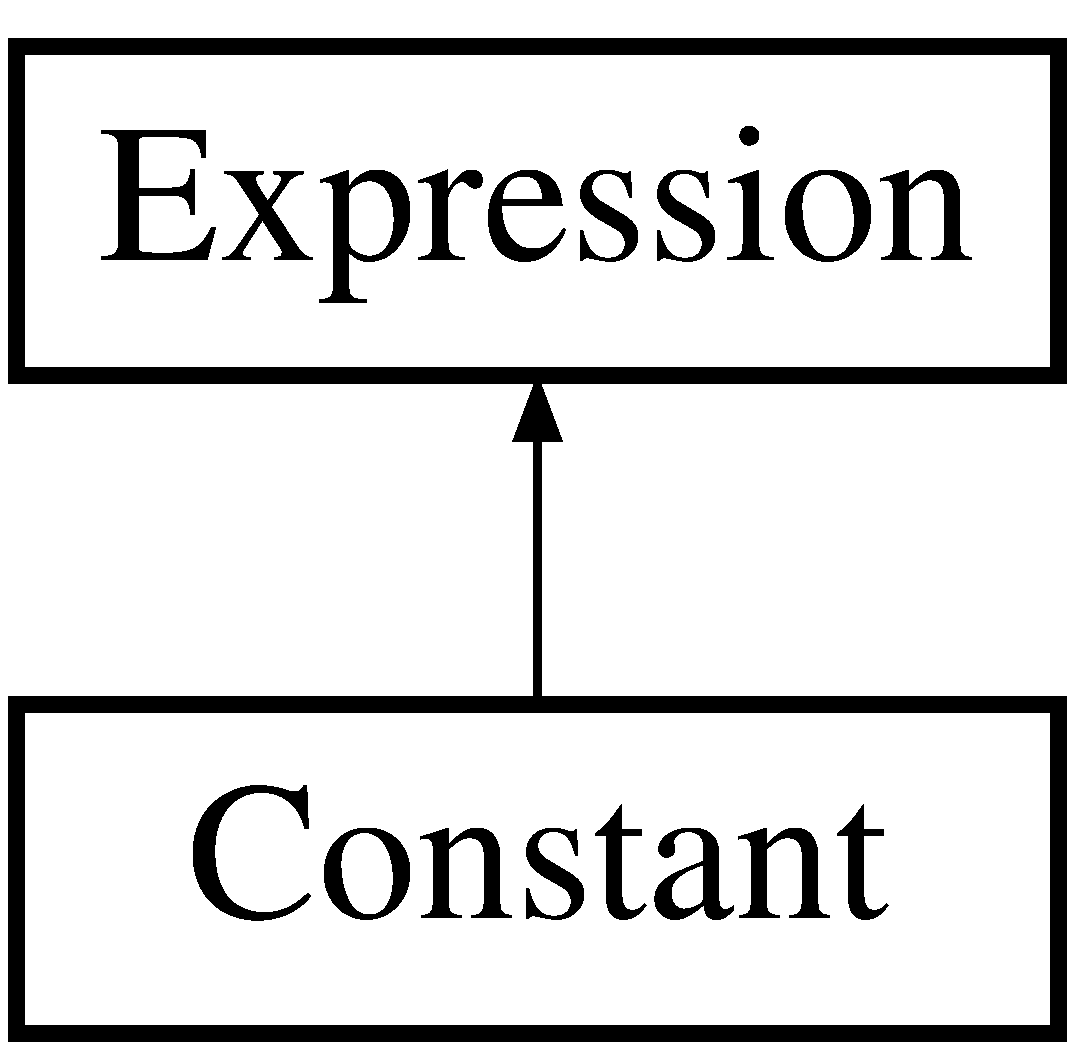
\includegraphics[height=2.000000cm]{class_constant}
\end{center}
\end{figure}
\subsection*{Public Member Functions}
\begin{DoxyCompactItemize}
\item 
Q\-String {\bf get\-Constant} ()
\item 
{\bf Constant} (Q\-String s)
\item 
const {\bf Nombre} \& {\bf evaluer} () const 
\item 
Q\-String {\bf get\-Propriete} ()
\end{DoxyCompactItemize}
\subsection*{Protected Attributes}
\begin{DoxyCompactItemize}
\item 
Q\-String {\bf constant}
\end{DoxyCompactItemize}


\subsection{Constructor \& Destructor Documentation}
\index{Constant@{Constant}!Constant@{Constant}}
\index{Constant@{Constant}!Constant@{Constant}}
\subsubsection[{Constant}]{\setlength{\rightskip}{0pt plus 5cm}Constant\-::\-Constant (
\begin{DoxyParamCaption}
\item[{Q\-String}]{s}
\end{DoxyParamCaption}
)\hspace{0.3cm}{\ttfamily [inline]}}\label{class_constant_aa794d00393c85db443cff7c0cdbbd4ca}


\subsection{Member Function Documentation}
\index{Constant@{Constant}!evaluer@{evaluer}}
\index{evaluer@{evaluer}!Constant@{Constant}}
\subsubsection[{evaluer}]{\setlength{\rightskip}{0pt plus 5cm}const {\bf Nombre} \& Constant\-::evaluer (
\begin{DoxyParamCaption}
{}
\end{DoxyParamCaption}
) const\hspace{0.3cm}{\ttfamily [virtual]}}\label{class_constant_a9042b3832b4573ab29a634b3f1758e93}


Implements {\bf Expression} \doxyref{}{p.}{class_expression_a883dfec27c4579cdd4749ce437d4925e}.

\index{Constant@{Constant}!get\-Constant@{get\-Constant}}
\index{get\-Constant@{get\-Constant}!Constant@{Constant}}
\subsubsection[{get\-Constant}]{\setlength{\rightskip}{0pt plus 5cm}Q\-String Constant\-::get\-Constant (
\begin{DoxyParamCaption}
{}
\end{DoxyParamCaption}
)\hspace{0.3cm}{\ttfamily [inline]}}\label{class_constant_a8682718b1084a4daac3d5700ec5261f3}
\index{Constant@{Constant}!get\-Propriete@{get\-Propriete}}
\index{get\-Propriete@{get\-Propriete}!Constant@{Constant}}
\subsubsection[{get\-Propriete}]{\setlength{\rightskip}{0pt plus 5cm}Q\-String Constant\-::get\-Propriete (
\begin{DoxyParamCaption}
{}
\end{DoxyParamCaption}
)\hspace{0.3cm}{\ttfamily [inline]}, {\ttfamily [virtual]}}\label{class_constant_ae7a03bc099618ca7004bf7c5a2da06c9}


Implements {\bf Expression} \doxyref{}{p.}{class_expression_a5c2940c8ca5195f5b9a51234c936e48c}.



\subsection{Member Data Documentation}
\index{Constant@{Constant}!constant@{constant}}
\index{constant@{constant}!Constant@{Constant}}
\subsubsection[{constant}]{\setlength{\rightskip}{0pt plus 5cm}Q\-String Constant\-::constant\hspace{0.3cm}{\ttfamily [protected]}}\label{class_constant_ac46faf278a29c49909758212ee957ed6}


The documentation for this class was generated from the following files\-:\begin{DoxyCompactItemize}
\item 
calculatrice/{\bf expression.\-h}\item 
calculatrice/{\bf expression.\-cpp}\end{DoxyCompactItemize}

\section{Entier Class Reference}
\label{class_entier}\index{Entier@{Entier}}


{\ttfamily \#include $<$expression.\-h$>$}

Inheritance diagram for Entier\-:\begin{figure}[H]
\begin{center}
\leavevmode
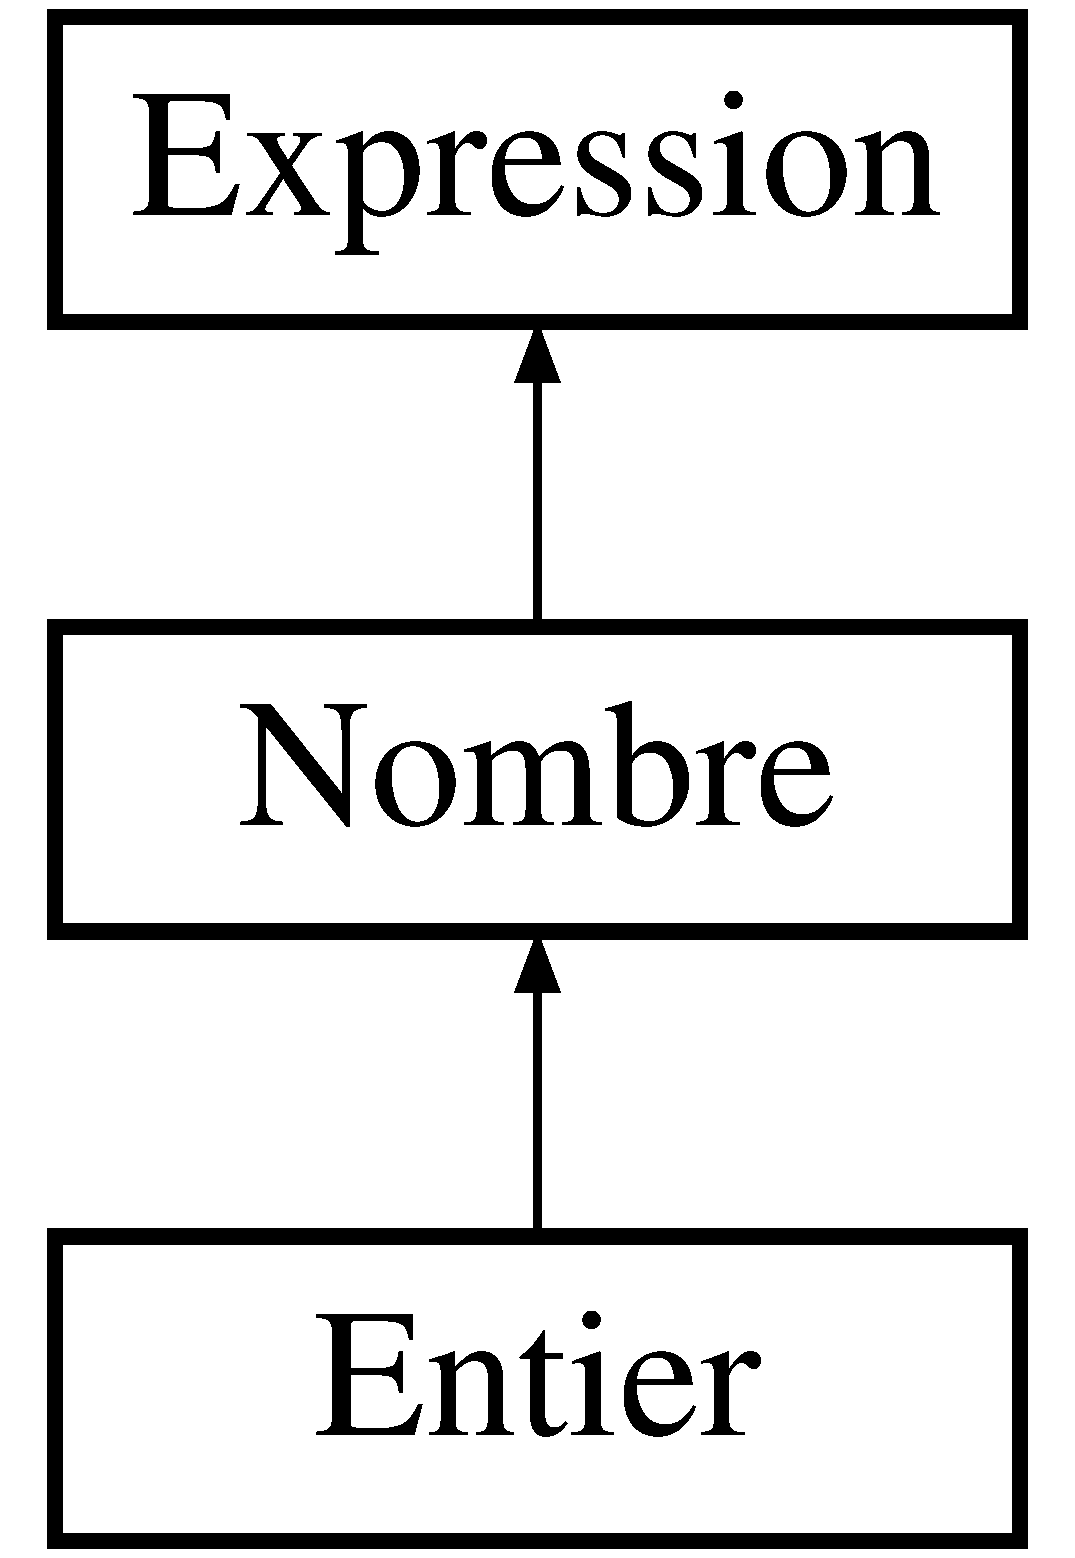
\includegraphics[height=3.000000cm]{class_entier}
\end{center}
\end{figure}
\subsection*{Public Member Functions}
\begin{DoxyCompactItemize}
\item 
{\bf Entier} (int valeur)
\item 
{\bf Entier} ()
\item 
const {\bf Entier} \& {\bf evaluer} () const 
\item 
Q\-String {\bf get\-Propriete} ()
\item 
{\bf Entier} \& {\bf operator=} (const {\bf Entier} \&e)
\item 
{\bf Nombre} \& {\bf operator+} (const {\bf Nombre} \&n)
\item 
{\bf Nombre} \& {\bf operator-\/} (const {\bf Nombre} \&n)
\item 
{\bf Nombre} \& {\bf operator$\ast$} (const {\bf Nombre} \&n)
\item 
{\bf Nombre} \& {\bf operator/} (const {\bf Nombre} \&n)
\end{DoxyCompactItemize}
\subsection*{Additional Inherited Members}


\subsection{Constructor \& Destructor Documentation}
\index{Entier@{Entier}!Entier@{Entier}}
\index{Entier@{Entier}!Entier@{Entier}}
\subsubsection[{Entier}]{\setlength{\rightskip}{0pt plus 5cm}Entier\-::\-Entier (
\begin{DoxyParamCaption}
\item[{int}]{valeur}
\end{DoxyParamCaption}
)}\label{class_entier_ac1410c4666b7577fa29b551be24819e6}
\index{Entier@{Entier}!Entier@{Entier}}
\index{Entier@{Entier}!Entier@{Entier}}
\subsubsection[{Entier}]{\setlength{\rightskip}{0pt plus 5cm}Entier\-::\-Entier (
\begin{DoxyParamCaption}
{}
\end{DoxyParamCaption}
)\hspace{0.3cm}{\ttfamily [inline]}}\label{class_entier_a1f0c17b51099803a73a4ec240c5587db}


\subsection{Member Function Documentation}
\index{Entier@{Entier}!evaluer@{evaluer}}
\index{evaluer@{evaluer}!Entier@{Entier}}
\subsubsection[{evaluer}]{\setlength{\rightskip}{0pt plus 5cm}const {\bf Entier} \& Entier\-::evaluer (
\begin{DoxyParamCaption}
{}
\end{DoxyParamCaption}
) const\hspace{0.3cm}{\ttfamily [virtual]}}\label{class_entier_a420df589673c97240bd8fca9daae3b9d}


Implements {\bf Expression} \doxyref{}{p.}{class_expression_a883dfec27c4579cdd4749ce437d4925e}.

\index{Entier@{Entier}!get\-Propriete@{get\-Propriete}}
\index{get\-Propriete@{get\-Propriete}!Entier@{Entier}}
\subsubsection[{get\-Propriete}]{\setlength{\rightskip}{0pt plus 5cm}Q\-String Entier\-::get\-Propriete (
\begin{DoxyParamCaption}
{}
\end{DoxyParamCaption}
)\hspace{0.3cm}{\ttfamily [inline]}, {\ttfamily [virtual]}}\label{class_entier_a908b0cab8111cfe22a9c355e2165c902}


Implements {\bf Expression} \doxyref{}{p.}{class_expression_a5c2940c8ca5195f5b9a51234c936e48c}.

\index{Entier@{Entier}!operator$\ast$@{operator$\ast$}}
\index{operator$\ast$@{operator$\ast$}!Entier@{Entier}}
\subsubsection[{operator$\ast$}]{\setlength{\rightskip}{0pt plus 5cm}{\bf Nombre} \& Entier\-::operator$\ast$ (
\begin{DoxyParamCaption}
\item[{const {\bf Nombre} \&}]{n}
\end{DoxyParamCaption}
)\hspace{0.3cm}{\ttfamily [virtual]}}\label{class_entier_aa16067ec35cbf26d7dfe949671622ae9}


Implements {\bf Nombre} \doxyref{}{p.}{class_nombre_ad249cd1678294bd419da8586ac9fbaa7}.

\index{Entier@{Entier}!operator+@{operator+}}
\index{operator+@{operator+}!Entier@{Entier}}
\subsubsection[{operator+}]{\setlength{\rightskip}{0pt plus 5cm}{\bf Nombre} \& Entier\-::operator+ (
\begin{DoxyParamCaption}
\item[{const {\bf Nombre} \&}]{n}
\end{DoxyParamCaption}
)\hspace{0.3cm}{\ttfamily [virtual]}}\label{class_entier_aff0d44c1db6a858e0975825303fe7863}


Implements {\bf Nombre} \doxyref{}{p.}{class_nombre_a8672fd34bb479f72a9479c146cb33b48}.

\index{Entier@{Entier}!operator-\/@{operator-\/}}
\index{operator-\/@{operator-\/}!Entier@{Entier}}
\subsubsection[{operator-\/}]{\setlength{\rightskip}{0pt plus 5cm}{\bf Nombre} \& Entier\-::operator-\/ (
\begin{DoxyParamCaption}
\item[{const {\bf Nombre} \&}]{n}
\end{DoxyParamCaption}
)\hspace{0.3cm}{\ttfamily [virtual]}}\label{class_entier_a2ed3580c21f9139ec0646c4f6edaed29}


Implements {\bf Nombre} \doxyref{}{p.}{class_nombre_a5a281bdf0efbc2a9b557abb8a58e8530}.

\index{Entier@{Entier}!operator/@{operator/}}
\index{operator/@{operator/}!Entier@{Entier}}
\subsubsection[{operator/}]{\setlength{\rightskip}{0pt plus 5cm}{\bf Nombre} \& Entier\-::operator/ (
\begin{DoxyParamCaption}
\item[{const {\bf Nombre} \&}]{n}
\end{DoxyParamCaption}
)\hspace{0.3cm}{\ttfamily [virtual]}}\label{class_entier_a4611824ea27d95d789c884597e75e832}


Implements {\bf Nombre} \doxyref{}{p.}{class_nombre_a7b55aa0d106bbb34001161fe6e7b8ebc}.

\index{Entier@{Entier}!operator=@{operator=}}
\index{operator=@{operator=}!Entier@{Entier}}
\subsubsection[{operator=}]{\setlength{\rightskip}{0pt plus 5cm}{\bf Entier} \& Entier\-::operator= (
\begin{DoxyParamCaption}
\item[{const {\bf Entier} \&}]{e}
\end{DoxyParamCaption}
)}\label{class_entier_a37577be01b8cd67ef5b76aad6240e5b6}


The documentation for this class was generated from the following files\-:\begin{DoxyCompactItemize}
\item 
calculatrice/{\bf expression.\-h}\item 
calculatrice/{\bf expression.\-cpp}\end{DoxyCompactItemize}

\section{Expression Class Reference}
\label{class_expression}\index{Expression@{Expression}}


{\ttfamily \#include $<$expression.\-h$>$}

Inheritance diagram for Expression\-:\begin{figure}[H]
\begin{center}
\leavevmode
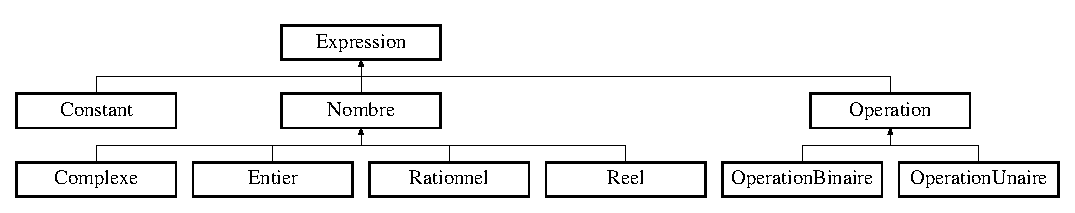
\includegraphics[height=2.413793cm]{class_expression}
\end{center}
\end{figure}
\subsection*{Public Member Functions}
\begin{DoxyCompactItemize}
\item 
virtual const {\bf Nombre} \& {\bf evaluer} () const =0
\item 
virtual Q\-String {\bf get\-Propriete} ()=0
\item 
virtual {\bf $\sim$\-Expression} ()
\end{DoxyCompactItemize}


\subsection{Constructor \& Destructor Documentation}
\index{Expression@{Expression}!$\sim$\-Expression@{$\sim$\-Expression}}
\index{$\sim$\-Expression@{$\sim$\-Expression}!Expression@{Expression}}
\subsubsection[{$\sim$\-Expression}]{\setlength{\rightskip}{0pt plus 5cm}virtual Expression\-::$\sim$\-Expression (
\begin{DoxyParamCaption}
{}
\end{DoxyParamCaption}
)\hspace{0.3cm}{\ttfamily [inline]}, {\ttfamily [virtual]}}\label{class_expression_a2f6cee3469dea6cbc3e5af93587f7c25}


\subsection{Member Function Documentation}
\index{Expression@{Expression}!evaluer@{evaluer}}
\index{evaluer@{evaluer}!Expression@{Expression}}
\subsubsection[{evaluer}]{\setlength{\rightskip}{0pt plus 5cm}virtual const {\bf Nombre}\& Expression\-::evaluer (
\begin{DoxyParamCaption}
{}
\end{DoxyParamCaption}
) const\hspace{0.3cm}{\ttfamily [pure virtual]}}\label{class_expression_a883dfec27c4579cdd4749ce437d4925e}


Implemented in {\bf Operation\-Unaire} \doxyref{}{p.}{class_operation_unaire_a3502d69ea658c0c5ea07a7b35a1238a8}, {\bf Operation\-Binaire} \doxyref{}{p.}{class_operation_binaire_a79548747f1afad38f99931a1e0920ab3}, {\bf Entier} \doxyref{}{p.}{class_entier_a420df589673c97240bd8fca9daae3b9d}, {\bf Rationnel} \doxyref{}{p.}{class_rationnel_ab88e2a4fbfbc0636be29c071318c9a7d}, {\bf Reel} \doxyref{}{p.}{class_reel_a880146cec8912d8e959baf46b2d2073b}, {\bf Complexe} \doxyref{}{p.}{class_complexe_a40c3fe088e4be07c905801596728ecce}, and {\bf Constant} \doxyref{}{p.}{class_constant_a9042b3832b4573ab29a634b3f1758e93}.

\index{Expression@{Expression}!get\-Propriete@{get\-Propriete}}
\index{get\-Propriete@{get\-Propriete}!Expression@{Expression}}
\subsubsection[{get\-Propriete}]{\setlength{\rightskip}{0pt plus 5cm}virtual Q\-String Expression\-::get\-Propriete (
\begin{DoxyParamCaption}
{}
\end{DoxyParamCaption}
)\hspace{0.3cm}{\ttfamily [pure virtual]}}\label{class_expression_a5c2940c8ca5195f5b9a51234c936e48c}


Implemented in {\bf Operation\-Unaire} \doxyref{}{p.}{class_operation_unaire_aa29a6fcf0c8e22aa6794177f42f7909a}, {\bf Operation\-Binaire} \doxyref{}{p.}{class_operation_binaire_af05041b13930db8501df8a07c92e1ff5}, {\bf Entier} \doxyref{}{p.}{class_entier_a908b0cab8111cfe22a9c355e2165c902}, {\bf Rationnel} \doxyref{}{p.}{class_rationnel_a47401159f8637c867760db02e2912569}, {\bf Reel} \doxyref{}{p.}{class_reel_ae9cc37231ca8ae433989952ed63e1c98}, {\bf Complexe} \doxyref{}{p.}{class_complexe_a8cb62d7f0f5c0a1df7707362cd19d9b9}, and {\bf Constant} \doxyref{}{p.}{class_constant_ae7a03bc099618ca7004bf7c5a2da06c9}.



The documentation for this class was generated from the following file\-:\begin{DoxyCompactItemize}
\item 
calculatrice/{\bf expression.\-h}\end{DoxyCompactItemize}

\section{Ui\-:\-:Main\-Window Class Reference}
\label{class_ui_1_1_main_window}\index{Ui\-::\-Main\-Window@{Ui\-::\-Main\-Window}}


{\ttfamily \#include $<$ui\-\_\-mainwindow.\-h$>$}

Inheritance diagram for Ui\-:\-:Main\-Window\-:\begin{figure}[H]
\begin{center}
\leavevmode
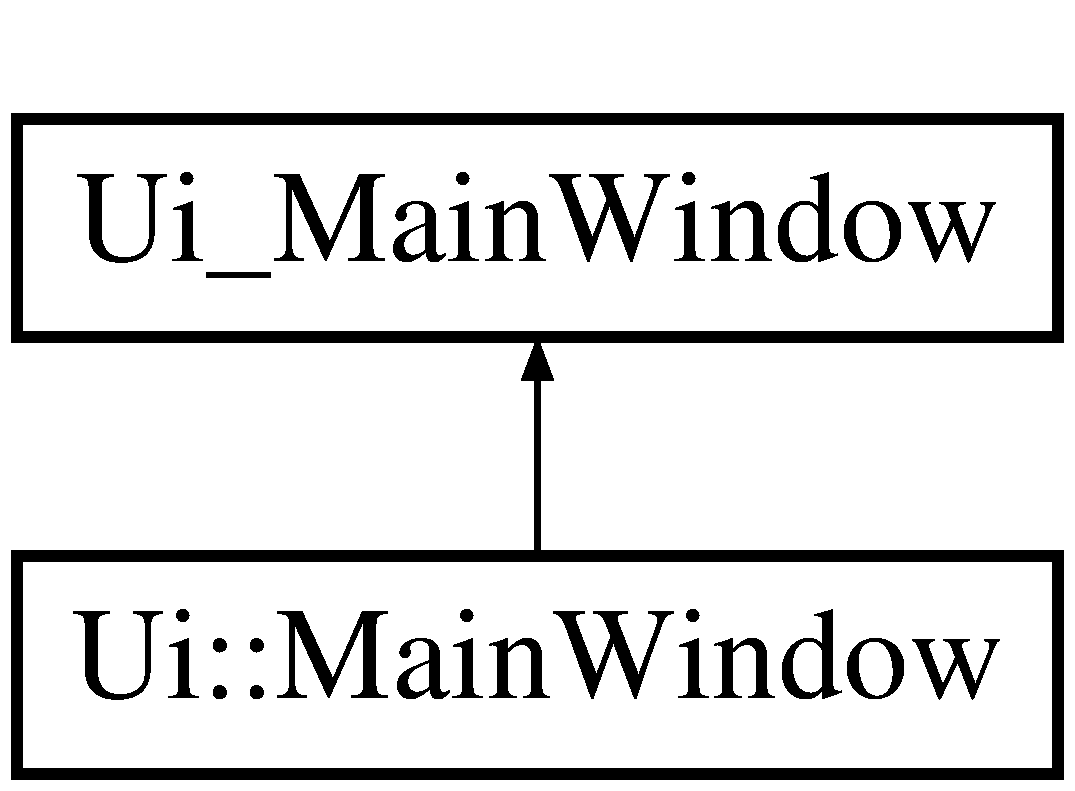
\includegraphics[height=2.000000cm]{class_ui_1_1_main_window}
\end{center}
\end{figure}
\subsection*{Additional Inherited Members}


The documentation for this class was generated from the following file\-:\begin{DoxyCompactItemize}
\item 
calculatrice/{\bf ui\-\_\-mainwindow.\-h}\end{DoxyCompactItemize}

\section{Main\-Window Class Reference}
\label{class_main_window}\index{Main\-Window@{Main\-Window}}


{\ttfamily \#include $<$mainwindow.\-h$>$}

\subsection*{Public Member Functions}
\begin{DoxyCompactItemize}
\item 
{\bf Main\-Window} (Q\-Widget $\ast$parent=0)
\item 
{\bf $\sim$\-Main\-Window} ()
\end{DoxyCompactItemize}
\subsection*{Public Attributes}
\begin{DoxyCompactItemize}
\item 
{\bf Pile} $\ast$ {\bf tempo}
\item 
{\bf Pile} $\ast$ {\bf historique}
\end{DoxyCompactItemize}


\subsection{Constructor \& Destructor Documentation}
\index{Main\-Window@{Main\-Window}!Main\-Window@{Main\-Window}}
\index{Main\-Window@{Main\-Window}!MainWindow@{Main\-Window}}
\subsubsection[{Main\-Window}]{\setlength{\rightskip}{0pt plus 5cm}Main\-Window\-::\-Main\-Window (
\begin{DoxyParamCaption}
\item[{Q\-Widget $\ast$}]{parent = {\ttfamily 0}}
\end{DoxyParamCaption}
)\hspace{0.3cm}{\ttfamily [explicit]}}\label{class_main_window_a8b244be8b7b7db1b08de2a2acb9409db}
\index{Main\-Window@{Main\-Window}!$\sim$\-Main\-Window@{$\sim$\-Main\-Window}}
\index{$\sim$\-Main\-Window@{$\sim$\-Main\-Window}!MainWindow@{Main\-Window}}
\subsubsection[{$\sim$\-Main\-Window}]{\setlength{\rightskip}{0pt plus 5cm}Main\-Window\-::$\sim$\-Main\-Window (
\begin{DoxyParamCaption}
{}
\end{DoxyParamCaption}
)}\label{class_main_window_ae98d00a93bc118200eeef9f9bba1dba7}


\subsection{Member Data Documentation}
\index{Main\-Window@{Main\-Window}!historique@{historique}}
\index{historique@{historique}!MainWindow@{Main\-Window}}
\subsubsection[{historique}]{\setlength{\rightskip}{0pt plus 5cm}{\bf Pile}$\ast$ Main\-Window\-::historique}\label{class_main_window_ab1b383c0450ed46281225db931bb1fb1}
\index{Main\-Window@{Main\-Window}!tempo@{tempo}}
\index{tempo@{tempo}!MainWindow@{Main\-Window}}
\subsubsection[{tempo}]{\setlength{\rightskip}{0pt plus 5cm}{\bf Pile}$\ast$ Main\-Window\-::tempo}\label{class_main_window_af43164f6e0a0a75422a2f574a39699b6}


The documentation for this class was generated from the following files\-:\begin{DoxyCompactItemize}
\item 
calculatrice/{\bf mainwindow.\-h}\item 
calculatrice/{\bf mainwindow.\-cpp}\end{DoxyCompactItemize}

\section{Nombre Class Reference}
\label{class_nombre}\index{Nombre@{Nombre}}


{\ttfamily \#include $<$expression.\-h$>$}

Inheritance diagram for Nombre\-:\begin{figure}[H]
\begin{center}
\leavevmode
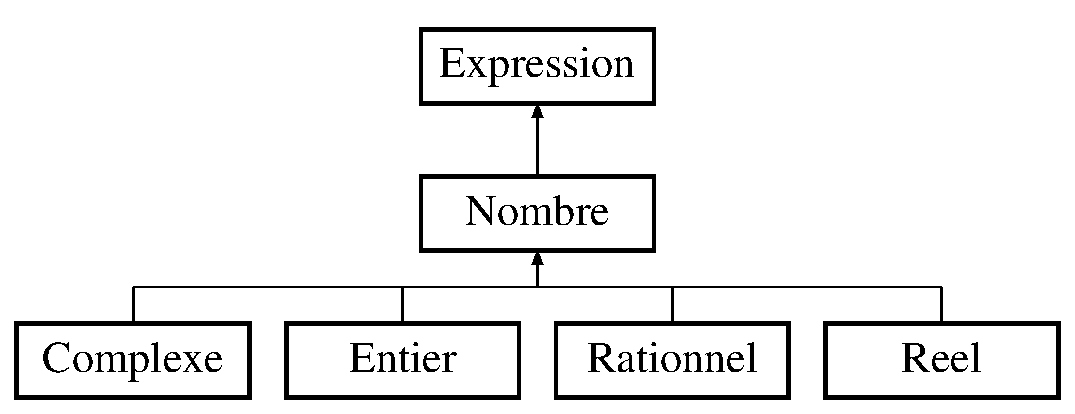
\includegraphics[height=3.000000cm]{class_nombre}
\end{center}
\end{figure}
\subsection*{Public Member Functions}
\begin{DoxyCompactItemize}
\item 
{\bf Nombre} (double partie\-Reelle, double partie\-Imaginaire)
\item 
{\bf Nombre} (double valeur)
\item 
{\bf Nombre} (int numerateur, int denominateur)
\item 
{\bf Nombre} (int valeur)
\item 
{\bf Nombre} ()
\item 
double {\bf get\-Partie\-Reelle} () const 
\item 
double {\bf get\-Partie\-Imaginaire} () const 
\item 
int {\bf get\-Denominateur\-Reel} () const 
\item 
int {\bf get\-Denominateur\-Imaginaire} () const 
\item 
std\-::string {\bf get\-Mode} () const 
\item 
void {\bf set\-Partie\-Reelle} (double nombre\-Reel)
\item 
void {\bf set\-Partie\-Imaginaire} (double nombre\-Imaginaire)
\item 
void {\bf set\-Denominateur\-Reel} (int denominateur)
\item 
void {\bf set\-Denominateur\-Imaginaire} (int denominateur)
\item 
virtual {\bf Nombre} \& {\bf operator+} (const {\bf Nombre} \&n)=0
\item 
virtual {\bf Nombre} \& {\bf operator-\/} (const {\bf Nombre} \&n)=0
\item 
virtual {\bf Nombre} \& {\bf operator$\ast$} (const {\bf Nombre} \&n)=0
\item 
virtual {\bf Nombre} \& {\bf operator/} (const {\bf Nombre} \&n)=0
\item 
int {\bf match\-\_\-affiche} () const 
\end{DoxyCompactItemize}
\subsection*{Protected Member Functions}
\begin{DoxyCompactItemize}
\item 
void {\bf set\-Mode} (std\-::string mode)
\end{DoxyCompactItemize}
\subsection*{Protected Attributes}
\begin{DoxyCompactItemize}
\item 
double {\bf m\-\_\-partie\-Reelle}
\item 
double {\bf m\-\_\-partie\-Imaginaire}
\item 
int {\bf m\-\_\-denominateur\-Reel}
\item 
int {\bf m\-\_\-denominateur\-Imaginaire}
\item 
std\-::string {\bf m\-\_\-mode}
\end{DoxyCompactItemize}


\subsection{Constructor \& Destructor Documentation}
\index{Nombre@{Nombre}!Nombre@{Nombre}}
\index{Nombre@{Nombre}!Nombre@{Nombre}}
\subsubsection[{Nombre}]{\setlength{\rightskip}{0pt plus 5cm}Nombre\-::\-Nombre (
\begin{DoxyParamCaption}
\item[{double}]{partie\-Reelle, }
\item[{double}]{partie\-Imaginaire}
\end{DoxyParamCaption}
)}\label{class_nombre_a7e9cc7ed8b4abcac0a1ce5fc907c77a2}
\index{Nombre@{Nombre}!Nombre@{Nombre}}
\index{Nombre@{Nombre}!Nombre@{Nombre}}
\subsubsection[{Nombre}]{\setlength{\rightskip}{0pt plus 5cm}Nombre\-::\-Nombre (
\begin{DoxyParamCaption}
\item[{double}]{valeur}
\end{DoxyParamCaption}
)}\label{class_nombre_a3501a6327a125bcb258065db556906a9}
\index{Nombre@{Nombre}!Nombre@{Nombre}}
\index{Nombre@{Nombre}!Nombre@{Nombre}}
\subsubsection[{Nombre}]{\setlength{\rightskip}{0pt plus 5cm}Nombre\-::\-Nombre (
\begin{DoxyParamCaption}
\item[{int}]{numerateur, }
\item[{int}]{denominateur}
\end{DoxyParamCaption}
)}\label{class_nombre_a574481639561725fb1ab0caca83d7996}
\index{Nombre@{Nombre}!Nombre@{Nombre}}
\index{Nombre@{Nombre}!Nombre@{Nombre}}
\subsubsection[{Nombre}]{\setlength{\rightskip}{0pt plus 5cm}Nombre\-::\-Nombre (
\begin{DoxyParamCaption}
\item[{int}]{valeur}
\end{DoxyParamCaption}
)}\label{class_nombre_af7c4d156dd3d6ed1c373463a81e629cd}
\index{Nombre@{Nombre}!Nombre@{Nombre}}
\index{Nombre@{Nombre}!Nombre@{Nombre}}
\subsubsection[{Nombre}]{\setlength{\rightskip}{0pt plus 5cm}Nombre\-::\-Nombre (
\begin{DoxyParamCaption}
{}
\end{DoxyParamCaption}
)}\label{class_nombre_a3c74c643475c2df0e2ecafe93a1e113a}


\subsection{Member Function Documentation}
\index{Nombre@{Nombre}!get\-Denominateur\-Imaginaire@{get\-Denominateur\-Imaginaire}}
\index{get\-Denominateur\-Imaginaire@{get\-Denominateur\-Imaginaire}!Nombre@{Nombre}}
\subsubsection[{get\-Denominateur\-Imaginaire}]{\setlength{\rightskip}{0pt plus 5cm}int Nombre\-::get\-Denominateur\-Imaginaire (
\begin{DoxyParamCaption}
{}
\end{DoxyParamCaption}
) const\hspace{0.3cm}{\ttfamily [inline]}}\label{class_nombre_a7e9f80ea2e78fd9339473c5a645a297b}
\index{Nombre@{Nombre}!get\-Denominateur\-Reel@{get\-Denominateur\-Reel}}
\index{get\-Denominateur\-Reel@{get\-Denominateur\-Reel}!Nombre@{Nombre}}
\subsubsection[{get\-Denominateur\-Reel}]{\setlength{\rightskip}{0pt plus 5cm}int Nombre\-::get\-Denominateur\-Reel (
\begin{DoxyParamCaption}
{}
\end{DoxyParamCaption}
) const\hspace{0.3cm}{\ttfamily [inline]}}\label{class_nombre_a1c2c83ad650fea716a6039d31f697196}
\index{Nombre@{Nombre}!get\-Mode@{get\-Mode}}
\index{get\-Mode@{get\-Mode}!Nombre@{Nombre}}
\subsubsection[{get\-Mode}]{\setlength{\rightskip}{0pt plus 5cm}std\-::string Nombre\-::get\-Mode (
\begin{DoxyParamCaption}
{}
\end{DoxyParamCaption}
) const\hspace{0.3cm}{\ttfamily [inline]}}\label{class_nombre_a97ac5eb6ecf22c70e96a36102d39558a}
\index{Nombre@{Nombre}!get\-Partie\-Imaginaire@{get\-Partie\-Imaginaire}}
\index{get\-Partie\-Imaginaire@{get\-Partie\-Imaginaire}!Nombre@{Nombre}}
\subsubsection[{get\-Partie\-Imaginaire}]{\setlength{\rightskip}{0pt plus 5cm}double Nombre\-::get\-Partie\-Imaginaire (
\begin{DoxyParamCaption}
{}
\end{DoxyParamCaption}
) const\hspace{0.3cm}{\ttfamily [inline]}}\label{class_nombre_a2dbf86d2af1d66b824a44d6b8a570231}
\index{Nombre@{Nombre}!get\-Partie\-Reelle@{get\-Partie\-Reelle}}
\index{get\-Partie\-Reelle@{get\-Partie\-Reelle}!Nombre@{Nombre}}
\subsubsection[{get\-Partie\-Reelle}]{\setlength{\rightskip}{0pt plus 5cm}double Nombre\-::get\-Partie\-Reelle (
\begin{DoxyParamCaption}
{}
\end{DoxyParamCaption}
) const\hspace{0.3cm}{\ttfamily [inline]}}\label{class_nombre_ae4f44da2905b32919b25ad2598c2e5e6}
\index{Nombre@{Nombre}!match\-\_\-affiche@{match\-\_\-affiche}}
\index{match\-\_\-affiche@{match\-\_\-affiche}!Nombre@{Nombre}}
\subsubsection[{match\-\_\-affiche}]{\setlength{\rightskip}{0pt plus 5cm}int Nombre\-::match\-\_\-affiche (
\begin{DoxyParamCaption}
{}
\end{DoxyParamCaption}
) const\hspace{0.3cm}{\ttfamily [inline]}}\label{class_nombre_ae1416ecdf3cc3da94d7659bfab90246c}
\index{Nombre@{Nombre}!operator$\ast$@{operator$\ast$}}
\index{operator$\ast$@{operator$\ast$}!Nombre@{Nombre}}
\subsubsection[{operator$\ast$}]{\setlength{\rightskip}{0pt plus 5cm}virtual {\bf Nombre}\& Nombre\-::operator$\ast$ (
\begin{DoxyParamCaption}
\item[{const {\bf Nombre} \&}]{n}
\end{DoxyParamCaption}
)\hspace{0.3cm}{\ttfamily [pure virtual]}}\label{class_nombre_ad249cd1678294bd419da8586ac9fbaa7}


Implemented in {\bf Entier} \doxyref{}{p.}{class_entier_aa16067ec35cbf26d7dfe949671622ae9}, {\bf Rationnel} \doxyref{}{p.}{class_rationnel_a649025539ecd1c000e30736da7d577ee}, {\bf Reel} \doxyref{}{p.}{class_reel_a4937d8ec303a13148b9e446d463fec70}, and {\bf Complexe} \doxyref{}{p.}{class_complexe_a324a6de3198334550e8c704830ef4ce4}.

\index{Nombre@{Nombre}!operator+@{operator+}}
\index{operator+@{operator+}!Nombre@{Nombre}}
\subsubsection[{operator+}]{\setlength{\rightskip}{0pt plus 5cm}virtual {\bf Nombre}\& Nombre\-::operator+ (
\begin{DoxyParamCaption}
\item[{const {\bf Nombre} \&}]{n}
\end{DoxyParamCaption}
)\hspace{0.3cm}{\ttfamily [pure virtual]}}\label{class_nombre_a8672fd34bb479f72a9479c146cb33b48}


Implemented in {\bf Entier} \doxyref{}{p.}{class_entier_aff0d44c1db6a858e0975825303fe7863}, {\bf Rationnel} \doxyref{}{p.}{class_rationnel_adf77c6d02e6ead3de56cf1be9f756774}, {\bf Reel} \doxyref{}{p.}{class_reel_a02efe680d4baa8c1ca23e65020141767}, and {\bf Complexe} \doxyref{}{p.}{class_complexe_afb89aaf210d1f1b4ec021cff1a3e43a5}.

\index{Nombre@{Nombre}!operator-\/@{operator-\/}}
\index{operator-\/@{operator-\/}!Nombre@{Nombre}}
\subsubsection[{operator-\/}]{\setlength{\rightskip}{0pt plus 5cm}virtual {\bf Nombre}\& Nombre\-::operator-\/ (
\begin{DoxyParamCaption}
\item[{const {\bf Nombre} \&}]{n}
\end{DoxyParamCaption}
)\hspace{0.3cm}{\ttfamily [pure virtual]}}\label{class_nombre_a5a281bdf0efbc2a9b557abb8a58e8530}


Implemented in {\bf Entier} \doxyref{}{p.}{class_entier_a2ed3580c21f9139ec0646c4f6edaed29}, {\bf Rationnel} \doxyref{}{p.}{class_rationnel_af3fdd026f75f03db372df5db43d071cb}, {\bf Reel} \doxyref{}{p.}{class_reel_ac6d168e265360da5a89bf89a68908696}, and {\bf Complexe} \doxyref{}{p.}{class_complexe_af03cf172928fdd461f73ca90ad92826b}.

\index{Nombre@{Nombre}!operator/@{operator/}}
\index{operator/@{operator/}!Nombre@{Nombre}}
\subsubsection[{operator/}]{\setlength{\rightskip}{0pt plus 5cm}virtual {\bf Nombre}\& Nombre\-::operator/ (
\begin{DoxyParamCaption}
\item[{const {\bf Nombre} \&}]{n}
\end{DoxyParamCaption}
)\hspace{0.3cm}{\ttfamily [pure virtual]}}\label{class_nombre_a7b55aa0d106bbb34001161fe6e7b8ebc}


Implemented in {\bf Entier} \doxyref{}{p.}{class_entier_a4611824ea27d95d789c884597e75e832}, {\bf Rationnel} \doxyref{}{p.}{class_rationnel_a63d26b746a9b46ac13488a1be19fef6e}, {\bf Reel} \doxyref{}{p.}{class_reel_ad5fb3c1583c8213581d06e2aa8e1f6df}, and {\bf Complexe} \doxyref{}{p.}{class_complexe_a5944d0f6628b7d8828ea5300dfe30a48}.

\index{Nombre@{Nombre}!set\-Denominateur\-Imaginaire@{set\-Denominateur\-Imaginaire}}
\index{set\-Denominateur\-Imaginaire@{set\-Denominateur\-Imaginaire}!Nombre@{Nombre}}
\subsubsection[{set\-Denominateur\-Imaginaire}]{\setlength{\rightskip}{0pt plus 5cm}void Nombre\-::set\-Denominateur\-Imaginaire (
\begin{DoxyParamCaption}
\item[{int}]{denominateur}
\end{DoxyParamCaption}
)\hspace{0.3cm}{\ttfamily [inline]}}\label{class_nombre_ac98de35312d5d4896a6c6d36ad05a701}
\index{Nombre@{Nombre}!set\-Denominateur\-Reel@{set\-Denominateur\-Reel}}
\index{set\-Denominateur\-Reel@{set\-Denominateur\-Reel}!Nombre@{Nombre}}
\subsubsection[{set\-Denominateur\-Reel}]{\setlength{\rightskip}{0pt plus 5cm}void Nombre\-::set\-Denominateur\-Reel (
\begin{DoxyParamCaption}
\item[{int}]{denominateur}
\end{DoxyParamCaption}
)\hspace{0.3cm}{\ttfamily [inline]}}\label{class_nombre_a2432c43647714eeb42151d41b64a9484}
\index{Nombre@{Nombre}!set\-Mode@{set\-Mode}}
\index{set\-Mode@{set\-Mode}!Nombre@{Nombre}}
\subsubsection[{set\-Mode}]{\setlength{\rightskip}{0pt plus 5cm}void Nombre\-::set\-Mode (
\begin{DoxyParamCaption}
\item[{std\-::string}]{mode}
\end{DoxyParamCaption}
)\hspace{0.3cm}{\ttfamily [inline]}, {\ttfamily [protected]}}\label{class_nombre_acf9b26af0fbc41cda15aa3e6dc551b76}
\index{Nombre@{Nombre}!set\-Partie\-Imaginaire@{set\-Partie\-Imaginaire}}
\index{set\-Partie\-Imaginaire@{set\-Partie\-Imaginaire}!Nombre@{Nombre}}
\subsubsection[{set\-Partie\-Imaginaire}]{\setlength{\rightskip}{0pt plus 5cm}void Nombre\-::set\-Partie\-Imaginaire (
\begin{DoxyParamCaption}
\item[{double}]{nombre\-Imaginaire}
\end{DoxyParamCaption}
)\hspace{0.3cm}{\ttfamily [inline]}}\label{class_nombre_a2863db3383245913ffd71cc5e50c116c}
\index{Nombre@{Nombre}!set\-Partie\-Reelle@{set\-Partie\-Reelle}}
\index{set\-Partie\-Reelle@{set\-Partie\-Reelle}!Nombre@{Nombre}}
\subsubsection[{set\-Partie\-Reelle}]{\setlength{\rightskip}{0pt plus 5cm}void Nombre\-::set\-Partie\-Reelle (
\begin{DoxyParamCaption}
\item[{double}]{nombre\-Reel}
\end{DoxyParamCaption}
)\hspace{0.3cm}{\ttfamily [inline]}}\label{class_nombre_a070cb0e583fb9aba1b11a97eadd01e18}


\subsection{Member Data Documentation}
\index{Nombre@{Nombre}!m\-\_\-denominateur\-Imaginaire@{m\-\_\-denominateur\-Imaginaire}}
\index{m\-\_\-denominateur\-Imaginaire@{m\-\_\-denominateur\-Imaginaire}!Nombre@{Nombre}}
\subsubsection[{m\-\_\-denominateur\-Imaginaire}]{\setlength{\rightskip}{0pt plus 5cm}int Nombre\-::m\-\_\-denominateur\-Imaginaire\hspace{0.3cm}{\ttfamily [protected]}}\label{class_nombre_ae4548d6e7bb285fc920b71b0949c8407}
\index{Nombre@{Nombre}!m\-\_\-denominateur\-Reel@{m\-\_\-denominateur\-Reel}}
\index{m\-\_\-denominateur\-Reel@{m\-\_\-denominateur\-Reel}!Nombre@{Nombre}}
\subsubsection[{m\-\_\-denominateur\-Reel}]{\setlength{\rightskip}{0pt plus 5cm}int Nombre\-::m\-\_\-denominateur\-Reel\hspace{0.3cm}{\ttfamily [protected]}}\label{class_nombre_a0fdd69b294016019fa19820bd8f53f82}
\index{Nombre@{Nombre}!m\-\_\-mode@{m\-\_\-mode}}
\index{m\-\_\-mode@{m\-\_\-mode}!Nombre@{Nombre}}
\subsubsection[{m\-\_\-mode}]{\setlength{\rightskip}{0pt plus 5cm}std\-::string Nombre\-::m\-\_\-mode\hspace{0.3cm}{\ttfamily [protected]}}\label{class_nombre_a1693034f58c00074cc9ffd1b8cc45b3a}
\index{Nombre@{Nombre}!m\-\_\-partie\-Imaginaire@{m\-\_\-partie\-Imaginaire}}
\index{m\-\_\-partie\-Imaginaire@{m\-\_\-partie\-Imaginaire}!Nombre@{Nombre}}
\subsubsection[{m\-\_\-partie\-Imaginaire}]{\setlength{\rightskip}{0pt plus 5cm}double Nombre\-::m\-\_\-partie\-Imaginaire\hspace{0.3cm}{\ttfamily [protected]}}\label{class_nombre_a1893bcb2b41d27dbedc5fb5aa0eda931}
\index{Nombre@{Nombre}!m\-\_\-partie\-Reelle@{m\-\_\-partie\-Reelle}}
\index{m\-\_\-partie\-Reelle@{m\-\_\-partie\-Reelle}!Nombre@{Nombre}}
\subsubsection[{m\-\_\-partie\-Reelle}]{\setlength{\rightskip}{0pt plus 5cm}double Nombre\-::m\-\_\-partie\-Reelle\hspace{0.3cm}{\ttfamily [protected]}}\label{class_nombre_a9b8eee6c056d760e299d7a370ad859f0}


The documentation for this class was generated from the following files\-:\begin{DoxyCompactItemize}
\item 
calculatrice/{\bf expression.\-h}\item 
calculatrice/{\bf expression.\-cpp}\end{DoxyCompactItemize}

\section{Operation Class Reference}
\label{class_operation}\index{Operation@{Operation}}


{\ttfamily \#include $<$expression.\-h$>$}

Inheritance diagram for Operation\-:\begin{figure}[H]
\begin{center}
\leavevmode
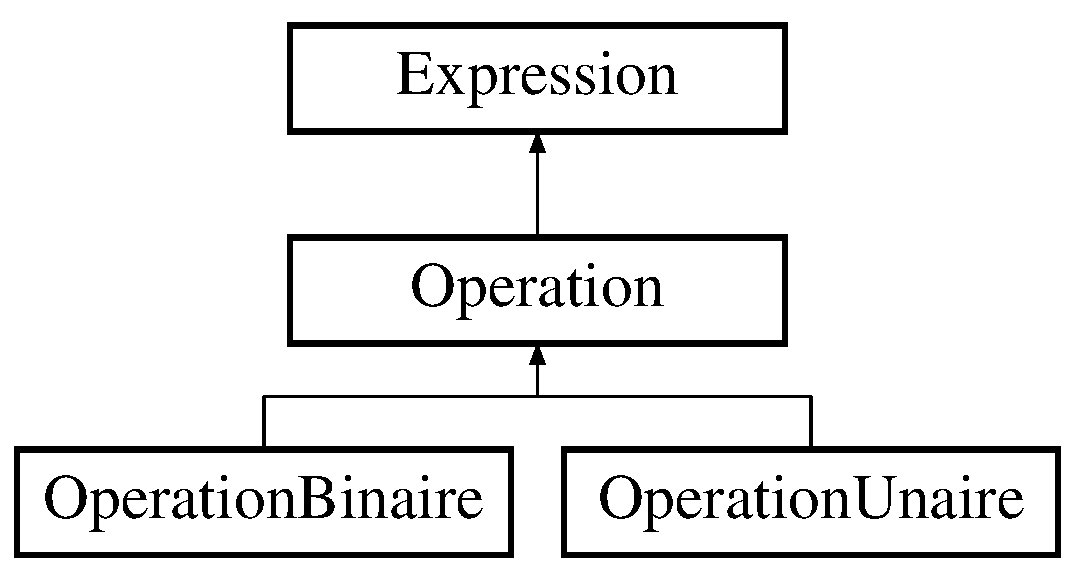
\includegraphics[height=3.000000cm]{class_operation}
\end{center}
\end{figure}
\subsection*{Public Member Functions}
\begin{DoxyCompactItemize}
\item 
{\bf Operation} (int indice)
\item 
int {\bf get\-Indice} () const 
\item 
Q\-String {\bf match\-\_\-indice} (int indice)
\end{DoxyCompactItemize}
\subsection*{Protected Attributes}
\begin{DoxyCompactItemize}
\item 
int {\bf choix}
\end{DoxyCompactItemize}


\subsection{Constructor \& Destructor Documentation}
\index{Operation@{Operation}!Operation@{Operation}}
\index{Operation@{Operation}!Operation@{Operation}}
\subsubsection[{Operation}]{\setlength{\rightskip}{0pt plus 5cm}Operation\-::\-Operation (
\begin{DoxyParamCaption}
\item[{int}]{indice}
\end{DoxyParamCaption}
)\hspace{0.3cm}{\ttfamily [inline]}}\label{class_operation_a14727fd7f6971803fdf667b40ab9b5e9}


\subsection{Member Function Documentation}
\index{Operation@{Operation}!get\-Indice@{get\-Indice}}
\index{get\-Indice@{get\-Indice}!Operation@{Operation}}
\subsubsection[{get\-Indice}]{\setlength{\rightskip}{0pt plus 5cm}int Operation\-::get\-Indice (
\begin{DoxyParamCaption}
{}
\end{DoxyParamCaption}
) const\hspace{0.3cm}{\ttfamily [inline]}}\label{class_operation_a13e0f13057633caee8fbda3c8d6f16ea}
\index{Operation@{Operation}!match\-\_\-indice@{match\-\_\-indice}}
\index{match\-\_\-indice@{match\-\_\-indice}!Operation@{Operation}}
\subsubsection[{match\-\_\-indice}]{\setlength{\rightskip}{0pt plus 5cm}Q\-String Operation\-::match\-\_\-indice (
\begin{DoxyParamCaption}
\item[{int}]{indice}
\end{DoxyParamCaption}
)}\label{class_operation_a154f13a325a3053217ba359e7695f59a}


\subsection{Member Data Documentation}
\index{Operation@{Operation}!choix@{choix}}
\index{choix@{choix}!Operation@{Operation}}
\subsubsection[{choix}]{\setlength{\rightskip}{0pt plus 5cm}int Operation\-::choix\hspace{0.3cm}{\ttfamily [protected]}}\label{class_operation_a84bdd0e69b370d28bf2c5c5041110c1d}


The documentation for this class was generated from the following files\-:\begin{DoxyCompactItemize}
\item 
calculatrice/{\bf expression.\-h}\item 
calculatrice/{\bf expression.\-cpp}\end{DoxyCompactItemize}

\section{Operation\-Binaire Class Reference}
\label{class_operation_binaire}\index{Operation\-Binaire@{Operation\-Binaire}}


{\ttfamily \#include $<$expression.\-h$>$}

Inheritance diagram for Operation\-Binaire\-:\begin{figure}[H]
\begin{center}
\leavevmode
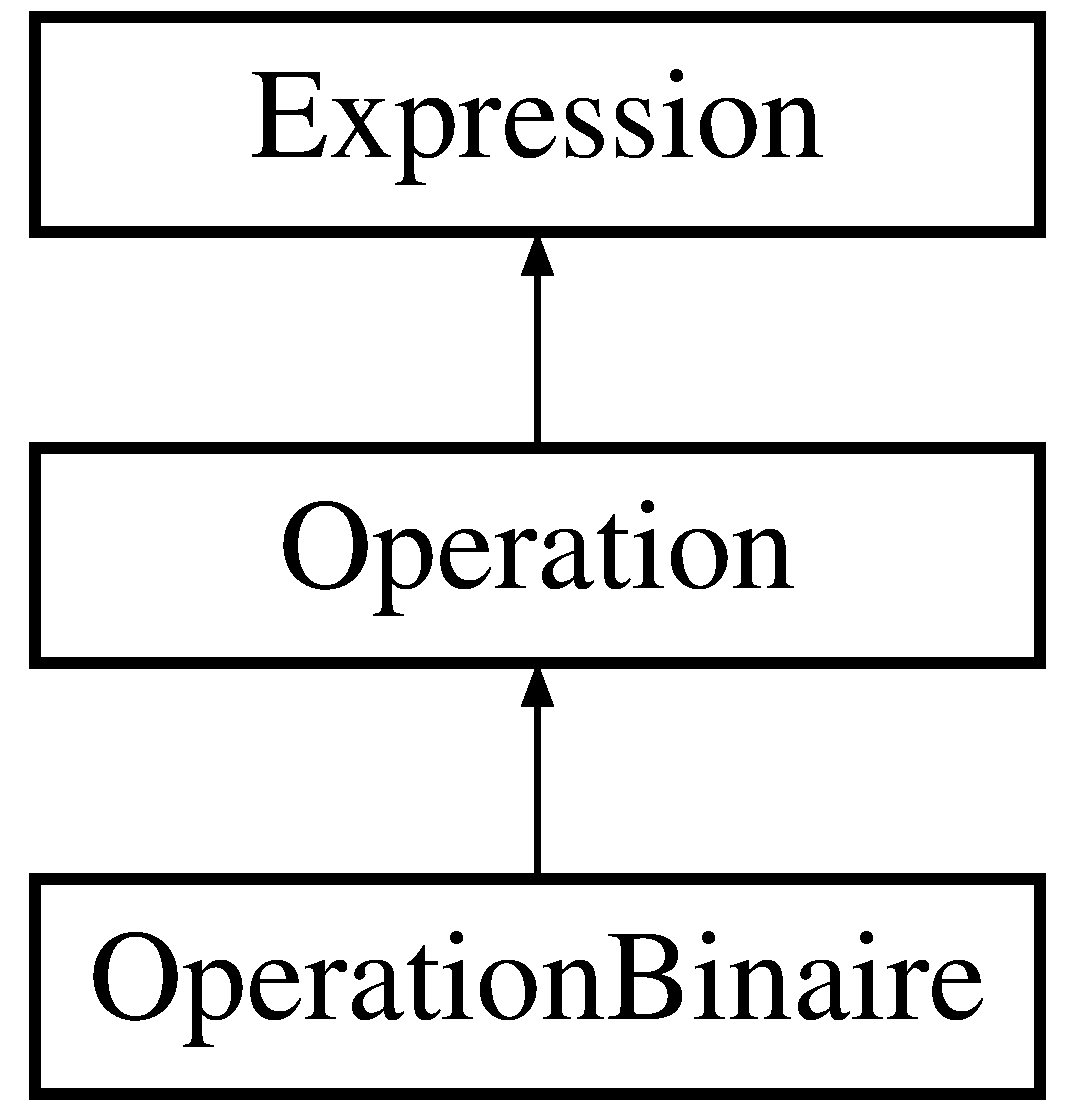
\includegraphics[height=3.000000cm]{class_operation_binaire}
\end{center}
\end{figure}
\subsection*{Public Member Functions}
\begin{DoxyCompactItemize}
\item 
{\bf Operation\-Binaire} ({\bf Expression} $\ast$x1, {\bf Expression} $\ast$x2, int indice)
\item 
const {\bf Nombre} \& {\bf evaluer} () const 
\item 
Q\-String {\bf get\-Propriete} ()
\item 
Q\-String {\bf get\-Result} ()
\item 
{\bf Expression} $\ast$ {\bf evaluer2} ()
\end{DoxyCompactItemize}
\subsection*{Additional Inherited Members}


\subsection{Constructor \& Destructor Documentation}
\index{Operation\-Binaire@{Operation\-Binaire}!Operation\-Binaire@{Operation\-Binaire}}
\index{Operation\-Binaire@{Operation\-Binaire}!OperationBinaire@{Operation\-Binaire}}
\subsubsection[{Operation\-Binaire}]{\setlength{\rightskip}{0pt plus 5cm}Operation\-Binaire\-::\-Operation\-Binaire (
\begin{DoxyParamCaption}
\item[{{\bf Expression} $\ast$}]{x1, }
\item[{{\bf Expression} $\ast$}]{x2, }
\item[{int}]{indice}
\end{DoxyParamCaption}
)\hspace{0.3cm}{\ttfamily [inline]}}\label{class_operation_binaire_a3e7144cfb9e325d8ebe4728aa433c59e}


\subsection{Member Function Documentation}
\index{Operation\-Binaire@{Operation\-Binaire}!evaluer@{evaluer}}
\index{evaluer@{evaluer}!OperationBinaire@{Operation\-Binaire}}
\subsubsection[{evaluer}]{\setlength{\rightskip}{0pt plus 5cm}const {\bf Nombre} \& Operation\-Binaire\-::evaluer (
\begin{DoxyParamCaption}
{}
\end{DoxyParamCaption}
) const\hspace{0.3cm}{\ttfamily [virtual]}}\label{class_operation_binaire_a79548747f1afad38f99931a1e0920ab3}


Implements {\bf Expression} \doxyref{}{p.}{class_expression_a883dfec27c4579cdd4749ce437d4925e}.

\index{Operation\-Binaire@{Operation\-Binaire}!evaluer2@{evaluer2}}
\index{evaluer2@{evaluer2}!OperationBinaire@{Operation\-Binaire}}
\subsubsection[{evaluer2}]{\setlength{\rightskip}{0pt plus 5cm}{\bf Expression} $\ast$ Operation\-Binaire\-::evaluer2 (
\begin{DoxyParamCaption}
{}
\end{DoxyParamCaption}
)}\label{class_operation_binaire_a8cd37f31aeed9033683fa118448d1330}
\index{Operation\-Binaire@{Operation\-Binaire}!get\-Propriete@{get\-Propriete}}
\index{get\-Propriete@{get\-Propriete}!OperationBinaire@{Operation\-Binaire}}
\subsubsection[{get\-Propriete}]{\setlength{\rightskip}{0pt plus 5cm}Q\-String Operation\-Binaire\-::get\-Propriete (
\begin{DoxyParamCaption}
{}
\end{DoxyParamCaption}
)\hspace{0.3cm}{\ttfamily [inline]}, {\ttfamily [virtual]}}\label{class_operation_binaire_af05041b13930db8501df8a07c92e1ff5}


Implements {\bf Expression} \doxyref{}{p.}{class_expression_a5c2940c8ca5195f5b9a51234c936e48c}.

\index{Operation\-Binaire@{Operation\-Binaire}!get\-Result@{get\-Result}}
\index{get\-Result@{get\-Result}!OperationBinaire@{Operation\-Binaire}}
\subsubsection[{get\-Result}]{\setlength{\rightskip}{0pt plus 5cm}Q\-String Operation\-Binaire\-::get\-Result (
\begin{DoxyParamCaption}
{}
\end{DoxyParamCaption}
)\hspace{0.3cm}{\ttfamily [inline]}}\label{class_operation_binaire_a7a676593741d779d9938747205db1685}


The documentation for this class was generated from the following files\-:\begin{DoxyCompactItemize}
\item 
calculatrice/{\bf expression.\-h}\item 
calculatrice/{\bf expression.\-cpp}\end{DoxyCompactItemize}

\section{Operation\-Unaire Class Reference}
\label{class_operation_unaire}\index{Operation\-Unaire@{Operation\-Unaire}}


{\ttfamily \#include $<$expression.\-h$>$}

Inheritance diagram for Operation\-Unaire\-:\begin{figure}[H]
\begin{center}
\leavevmode
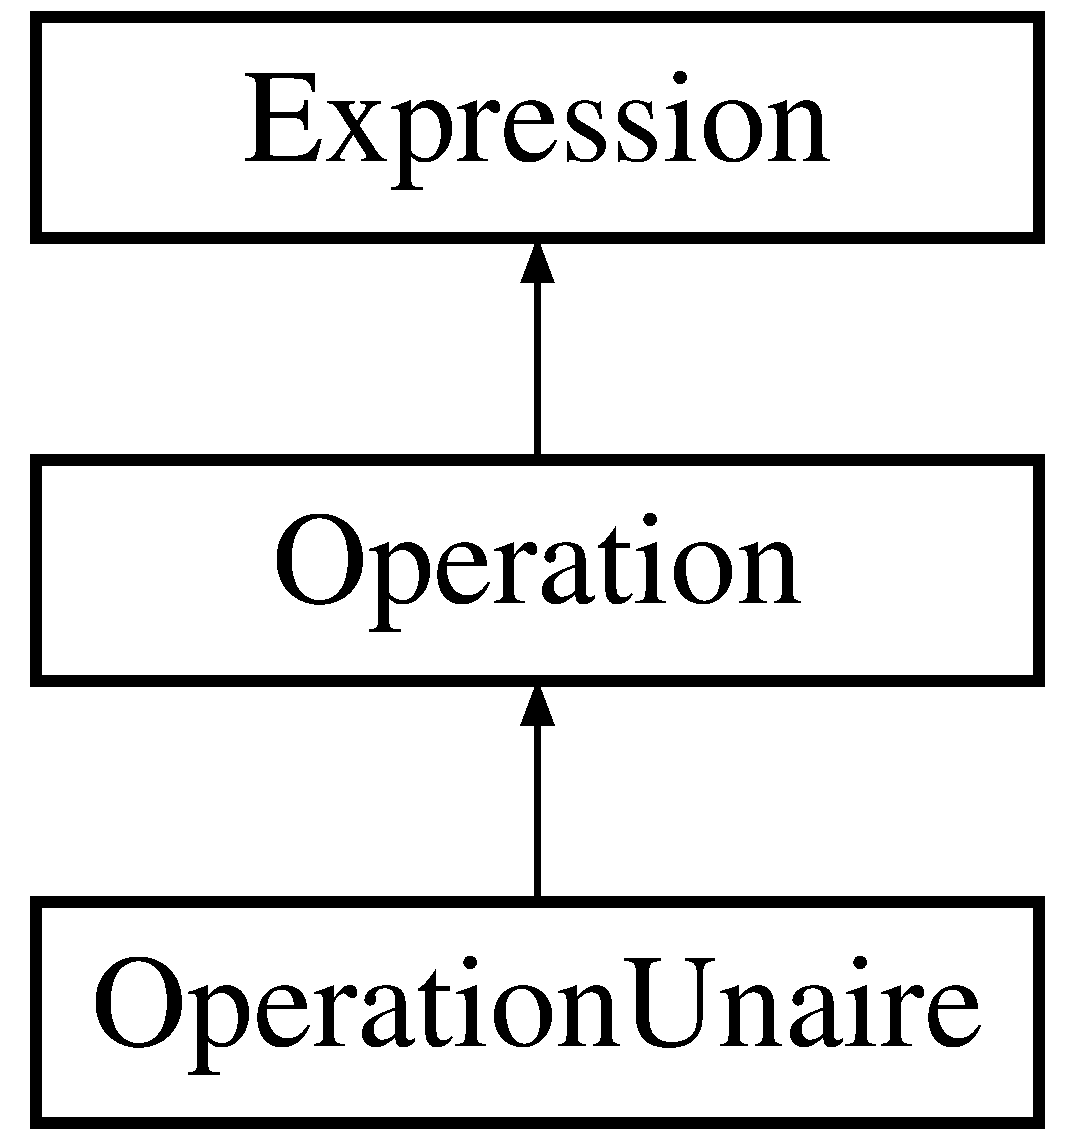
\includegraphics[height=3.000000cm]{class_operation_unaire}
\end{center}
\end{figure}
\subsection*{Public Member Functions}
\begin{DoxyCompactItemize}
\item 
{\bf Operation\-Unaire} ({\bf Expression} $\ast$x1, int indice)
\item 
const {\bf Nombre} \& {\bf evaluer} () const 
\item 
{\bf Expression} $\ast$ {\bf evaluer2} ()
\item 
Q\-String {\bf get\-Result} ()
\item 
Q\-String {\bf get\-Propriete} ()
\end{DoxyCompactItemize}
\subsection*{Additional Inherited Members}


\subsection{Constructor \& Destructor Documentation}
\index{Operation\-Unaire@{Operation\-Unaire}!Operation\-Unaire@{Operation\-Unaire}}
\index{Operation\-Unaire@{Operation\-Unaire}!OperationUnaire@{Operation\-Unaire}}
\subsubsection[{Operation\-Unaire}]{\setlength{\rightskip}{0pt plus 5cm}Operation\-Unaire\-::\-Operation\-Unaire (
\begin{DoxyParamCaption}
\item[{{\bf Expression} $\ast$}]{x1, }
\item[{int}]{indice}
\end{DoxyParamCaption}
)\hspace{0.3cm}{\ttfamily [inline]}}\label{class_operation_unaire_ae0bda26e4ea7483a9b42b35aca2b90a5}


\subsection{Member Function Documentation}
\index{Operation\-Unaire@{Operation\-Unaire}!evaluer@{evaluer}}
\index{evaluer@{evaluer}!OperationUnaire@{Operation\-Unaire}}
\subsubsection[{evaluer}]{\setlength{\rightskip}{0pt plus 5cm}const {\bf Nombre} \& Operation\-Unaire\-::evaluer (
\begin{DoxyParamCaption}
{}
\end{DoxyParamCaption}
) const\hspace{0.3cm}{\ttfamily [virtual]}}\label{class_operation_unaire_a3502d69ea658c0c5ea07a7b35a1238a8}


Implements {\bf Expression} \doxyref{}{p.}{class_expression_a883dfec27c4579cdd4749ce437d4925e}.

\index{Operation\-Unaire@{Operation\-Unaire}!evaluer2@{evaluer2}}
\index{evaluer2@{evaluer2}!OperationUnaire@{Operation\-Unaire}}
\subsubsection[{evaluer2}]{\setlength{\rightskip}{0pt plus 5cm}{\bf Expression} $\ast$ Operation\-Unaire\-::evaluer2 (
\begin{DoxyParamCaption}
{}
\end{DoxyParamCaption}
)}\label{class_operation_unaire_a20615438abfd13396f69a8d379e2a429}
\index{Operation\-Unaire@{Operation\-Unaire}!get\-Propriete@{get\-Propriete}}
\index{get\-Propriete@{get\-Propriete}!OperationUnaire@{Operation\-Unaire}}
\subsubsection[{get\-Propriete}]{\setlength{\rightskip}{0pt plus 5cm}Q\-String Operation\-Unaire\-::get\-Propriete (
\begin{DoxyParamCaption}
{}
\end{DoxyParamCaption}
)\hspace{0.3cm}{\ttfamily [inline]}, {\ttfamily [virtual]}}\label{class_operation_unaire_aa29a6fcf0c8e22aa6794177f42f7909a}


Implements {\bf Expression} \doxyref{}{p.}{class_expression_a5c2940c8ca5195f5b9a51234c936e48c}.

\index{Operation\-Unaire@{Operation\-Unaire}!get\-Result@{get\-Result}}
\index{get\-Result@{get\-Result}!OperationUnaire@{Operation\-Unaire}}
\subsubsection[{get\-Result}]{\setlength{\rightskip}{0pt plus 5cm}Q\-String Operation\-Unaire\-::get\-Result (
\begin{DoxyParamCaption}
{}
\end{DoxyParamCaption}
)\hspace{0.3cm}{\ttfamily [inline]}}\label{class_operation_unaire_a3d01de06d4d25ba0f282987aa724e473}


The documentation for this class was generated from the following files\-:\begin{DoxyCompactItemize}
\item 
calculatrice/{\bf expression.\-h}\item 
calculatrice/{\bf expression.\-cpp}\end{DoxyCompactItemize}

\section{Pile Class Reference}
\label{class_pile}\index{Pile@{Pile}}


{\ttfamily \#include $<$pile.\-h$>$}

\subsection*{Public Member Functions}
\begin{DoxyCompactItemize}
\item 
Q\-String {\bf get\-\_\-result} ()
\item 
Q\-String {\bf set\-\_\-result} (Q\-String s)
\item 
Q\-Stack$<$ {\bf Expression} $\ast$ $>$ {\bf get\-Element} ()
\item 
Q\-Stack$<$ Q\-String $>$ {\bf get\-Aff} ()
\item 
bool {\bf traitement} (Q\-String commande)
\item 
void {\bf swap} (int x, int y)
\item 
void {\bf sum} (int x)
\item 
void {\bf mean} (int x)
\item 
void {\bf clear} ()
\item 
void {\bf dup} ()
\item 
void {\bf drop} ()
\item 
void {\bf annuler} ()
\item 
void {\bf retablir} ()
\item 
void {\bf empiler\-\_\-\-Aff} (Q\-String s)
\item 
void {\bf empiler} ({\bf Expression} $\ast$s)
\item 
{\bf Expression} $\ast$ {\bf depiler} ()
\item 
void {\bf afficher} ()
\item 
Q\-String {\bf depiler\-\_\-\-Aff} ()
\item 
{\bf Pile} ()
\item 
{\bf $\sim$\-Pile} ()
\item 
int {\bf get\-\_\-m\-\_\-nombre\-Element} () const 
\end{DoxyCompactItemize}
\subsection*{Public Attributes}
\begin{DoxyCompactItemize}
\item 
Q\-Stack$<$ Q\-String $>$ {\bf Afficheur}
\end{DoxyCompactItemize}


\subsection{Constructor \& Destructor Documentation}
\index{Pile@{Pile}!Pile@{Pile}}
\index{Pile@{Pile}!Pile@{Pile}}
\subsubsection[{Pile}]{\setlength{\rightskip}{0pt plus 5cm}Pile\-::\-Pile (
\begin{DoxyParamCaption}
{}
\end{DoxyParamCaption}
)}\label{class_pile_ab44e927107b28f5f3ac7697d10e0a739}
\index{Pile@{Pile}!$\sim$\-Pile@{$\sim$\-Pile}}
\index{$\sim$\-Pile@{$\sim$\-Pile}!Pile@{Pile}}
\subsubsection[{$\sim$\-Pile}]{\setlength{\rightskip}{0pt plus 5cm}Pile\-::$\sim$\-Pile (
\begin{DoxyParamCaption}
{}
\end{DoxyParamCaption}
)}\label{class_pile_ab2d1398d675586ff34994e2b109df152}


\subsection{Member Function Documentation}
\index{Pile@{Pile}!afficher@{afficher}}
\index{afficher@{afficher}!Pile@{Pile}}
\subsubsection[{afficher}]{\setlength{\rightskip}{0pt plus 5cm}void Pile\-::afficher (
\begin{DoxyParamCaption}
{}
\end{DoxyParamCaption}
)}\label{class_pile_ade235ddd6a30f0920039690093ddfc33}
\index{Pile@{Pile}!annuler@{annuler}}
\index{annuler@{annuler}!Pile@{Pile}}
\subsubsection[{annuler}]{\setlength{\rightskip}{0pt plus 5cm}void Pile\-::annuler (
\begin{DoxyParamCaption}
{}
\end{DoxyParamCaption}
)}\label{class_pile_af8efea7a91f6403eab295577004ae620}
\index{Pile@{Pile}!clear@{clear}}
\index{clear@{clear}!Pile@{Pile}}
\subsubsection[{clear}]{\setlength{\rightskip}{0pt plus 5cm}void Pile\-::clear (
\begin{DoxyParamCaption}
{}
\end{DoxyParamCaption}
)}\label{class_pile_aa3991438f190580607d7bbbd50ecc0c3}
\index{Pile@{Pile}!depiler@{depiler}}
\index{depiler@{depiler}!Pile@{Pile}}
\subsubsection[{depiler}]{\setlength{\rightskip}{0pt plus 5cm}{\bf Expression} $\ast$ Pile\-::depiler (
\begin{DoxyParamCaption}
{}
\end{DoxyParamCaption}
)}\label{class_pile_ab9b9c6abfb90f060a38bb53b9118ce4b}
\index{Pile@{Pile}!depiler\-\_\-\-Aff@{depiler\-\_\-\-Aff}}
\index{depiler\-\_\-\-Aff@{depiler\-\_\-\-Aff}!Pile@{Pile}}
\subsubsection[{depiler\-\_\-\-Aff}]{\setlength{\rightskip}{0pt plus 5cm}Q\-String Pile\-::depiler\-\_\-\-Aff (
\begin{DoxyParamCaption}
{}
\end{DoxyParamCaption}
)}\label{class_pile_a2b1fb05097e51d7e332e957f0b5eab84}
\index{Pile@{Pile}!drop@{drop}}
\index{drop@{drop}!Pile@{Pile}}
\subsubsection[{drop}]{\setlength{\rightskip}{0pt plus 5cm}void Pile\-::drop (
\begin{DoxyParamCaption}
{}
\end{DoxyParamCaption}
)}\label{class_pile_a7488ed257c6ceb16ed57a9fffb0726d5}
\index{Pile@{Pile}!dup@{dup}}
\index{dup@{dup}!Pile@{Pile}}
\subsubsection[{dup}]{\setlength{\rightskip}{0pt plus 5cm}void Pile\-::dup (
\begin{DoxyParamCaption}
{}
\end{DoxyParamCaption}
)}\label{class_pile_a081f7843d01cae1f0f7be7d92e46d5d2}
\index{Pile@{Pile}!empiler@{empiler}}
\index{empiler@{empiler}!Pile@{Pile}}
\subsubsection[{empiler}]{\setlength{\rightskip}{0pt plus 5cm}void Pile\-::empiler (
\begin{DoxyParamCaption}
\item[{{\bf Expression} $\ast$}]{s}
\end{DoxyParamCaption}
)}\label{class_pile_ae557d09ac9527d0858821fa8a76847bc}
\index{Pile@{Pile}!empiler\-\_\-\-Aff@{empiler\-\_\-\-Aff}}
\index{empiler\-\_\-\-Aff@{empiler\-\_\-\-Aff}!Pile@{Pile}}
\subsubsection[{empiler\-\_\-\-Aff}]{\setlength{\rightskip}{0pt plus 5cm}void Pile\-::empiler\-\_\-\-Aff (
\begin{DoxyParamCaption}
\item[{Q\-String}]{s}
\end{DoxyParamCaption}
)}\label{class_pile_a6c26a20b4e947f6ef70aeb346e55c9d3}
\index{Pile@{Pile}!get\-\_\-m\-\_\-nombre\-Element@{get\-\_\-m\-\_\-nombre\-Element}}
\index{get\-\_\-m\-\_\-nombre\-Element@{get\-\_\-m\-\_\-nombre\-Element}!Pile@{Pile}}
\subsubsection[{get\-\_\-m\-\_\-nombre\-Element}]{\setlength{\rightskip}{0pt plus 5cm}int Pile\-::get\-\_\-m\-\_\-nombre\-Element (
\begin{DoxyParamCaption}
{}
\end{DoxyParamCaption}
) const\hspace{0.3cm}{\ttfamily [inline]}}\label{class_pile_ad390f27e14d4cda19d356dc4204b7e12}
\index{Pile@{Pile}!get\-\_\-result@{get\-\_\-result}}
\index{get\-\_\-result@{get\-\_\-result}!Pile@{Pile}}
\subsubsection[{get\-\_\-result}]{\setlength{\rightskip}{0pt plus 5cm}Q\-String Pile\-::get\-\_\-result (
\begin{DoxyParamCaption}
{}
\end{DoxyParamCaption}
)\hspace{0.3cm}{\ttfamily [inline]}}\label{class_pile_ae591cadce625ef96b61dbbb9e6358087}
\index{Pile@{Pile}!get\-Aff@{get\-Aff}}
\index{get\-Aff@{get\-Aff}!Pile@{Pile}}
\subsubsection[{get\-Aff}]{\setlength{\rightskip}{0pt plus 5cm}Q\-Stack$<$Q\-String$>$ Pile\-::get\-Aff (
\begin{DoxyParamCaption}
{}
\end{DoxyParamCaption}
)\hspace{0.3cm}{\ttfamily [inline]}}\label{class_pile_a3bfeb0fac8bf9bcf2f08b2b83353b32a}
\index{Pile@{Pile}!get\-Element@{get\-Element}}
\index{get\-Element@{get\-Element}!Pile@{Pile}}
\subsubsection[{get\-Element}]{\setlength{\rightskip}{0pt plus 5cm}Q\-Stack$<${\bf Expression} $\ast$$>$ Pile\-::get\-Element (
\begin{DoxyParamCaption}
{}
\end{DoxyParamCaption}
)\hspace{0.3cm}{\ttfamily [inline]}}\label{class_pile_ae1cce464d804eaf82dc6f588ceeafdbd}
\index{Pile@{Pile}!mean@{mean}}
\index{mean@{mean}!Pile@{Pile}}
\subsubsection[{mean}]{\setlength{\rightskip}{0pt plus 5cm}void Pile\-::mean (
\begin{DoxyParamCaption}
\item[{int}]{x}
\end{DoxyParamCaption}
)}\label{class_pile_a1daebba5bd1d6c6d79de63728cc892a9}
\index{Pile@{Pile}!retablir@{retablir}}
\index{retablir@{retablir}!Pile@{Pile}}
\subsubsection[{retablir}]{\setlength{\rightskip}{0pt plus 5cm}void Pile\-::retablir (
\begin{DoxyParamCaption}
{}
\end{DoxyParamCaption}
)}\label{class_pile_a36b0ff28bf644cebe2d336ebbb0a07ac}
\index{Pile@{Pile}!set\-\_\-result@{set\-\_\-result}}
\index{set\-\_\-result@{set\-\_\-result}!Pile@{Pile}}
\subsubsection[{set\-\_\-result}]{\setlength{\rightskip}{0pt plus 5cm}Q\-String Pile\-::set\-\_\-result (
\begin{DoxyParamCaption}
\item[{Q\-String}]{s}
\end{DoxyParamCaption}
)\hspace{0.3cm}{\ttfamily [inline]}}\label{class_pile_a2338a95c050d307fce0bf66f91c9a58b}
\index{Pile@{Pile}!sum@{sum}}
\index{sum@{sum}!Pile@{Pile}}
\subsubsection[{sum}]{\setlength{\rightskip}{0pt plus 5cm}void Pile\-::sum (
\begin{DoxyParamCaption}
\item[{int}]{x}
\end{DoxyParamCaption}
)}\label{class_pile_ae09e2cf01c21b58a6c2c4efee101c158}
\index{Pile@{Pile}!swap@{swap}}
\index{swap@{swap}!Pile@{Pile}}
\subsubsection[{swap}]{\setlength{\rightskip}{0pt plus 5cm}void Pile\-::swap (
\begin{DoxyParamCaption}
\item[{int}]{x, }
\item[{int}]{y}
\end{DoxyParamCaption}
)}\label{class_pile_a1a19ce2a4a6a76286fae8243a1f9e247}
\index{Pile@{Pile}!traitement@{traitement}}
\index{traitement@{traitement}!Pile@{Pile}}
\subsubsection[{traitement}]{\setlength{\rightskip}{0pt plus 5cm}bool Pile\-::traitement (
\begin{DoxyParamCaption}
\item[{Q\-String}]{commande}
\end{DoxyParamCaption}
)}\label{class_pile_a615ef5113bbfc42def6429c803a385c7}


\subsection{Member Data Documentation}
\index{Pile@{Pile}!Afficheur@{Afficheur}}
\index{Afficheur@{Afficheur}!Pile@{Pile}}
\subsubsection[{Afficheur}]{\setlength{\rightskip}{0pt plus 5cm}Q\-Stack$<$Q\-String$>$ Pile\-::\-Afficheur}\label{class_pile_ac5b403244fa24be19ce7066a3950dcc1}


The documentation for this class was generated from the following files\-:\begin{DoxyCompactItemize}
\item 
calculatrice/{\bf pile.\-h}\item 
calculatrice/{\bf pile.\-cpp}\end{DoxyCompactItemize}

\section{Rationnel Class Reference}
\label{class_rationnel}\index{Rationnel@{Rationnel}}


{\ttfamily \#include $<$expression.\-h$>$}

Inheritance diagram for Rationnel\-:\begin{figure}[H]
\begin{center}
\leavevmode
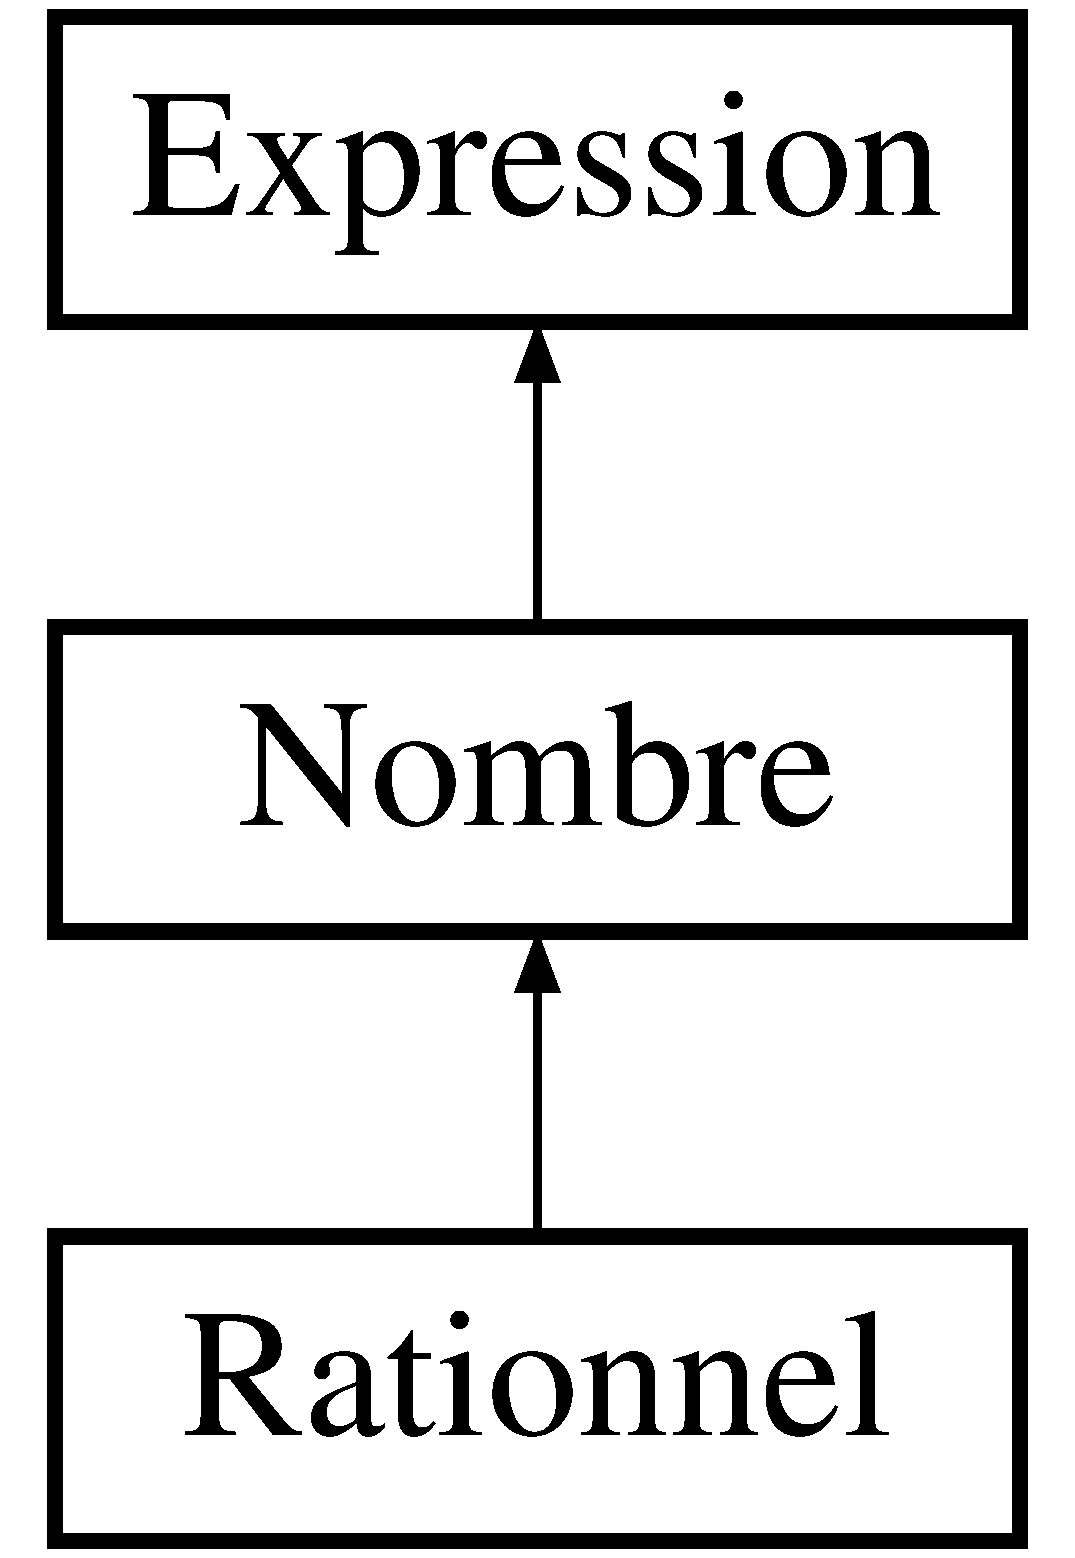
\includegraphics[height=3.000000cm]{class_rationnel}
\end{center}
\end{figure}
\subsection*{Public Member Functions}
\begin{DoxyCompactItemize}
\item 
{\bf Rationnel} (int numerateur, int denominateur)
\item 
{\bf Rationnel} ()
\item 
const {\bf Rationnel} \& {\bf evaluer} () const 
\item 
Q\-String {\bf get\-Propriete} ()
\item 
{\bf Rationnel} \& {\bf operator=} (const {\bf Rationnel} \&q)
\item 
{\bf Nombre} \& {\bf operator+} (const {\bf Nombre} \&n)
\item 
{\bf Nombre} \& {\bf operator-\/} (const {\bf Nombre} \&n)
\item 
{\bf Nombre} \& {\bf operator$\ast$} (const {\bf Nombre} \&n)
\item 
{\bf Nombre} \& {\bf operator/} (const {\bf Nombre} \&n)
\end{DoxyCompactItemize}
\subsection*{Additional Inherited Members}


\subsection{Constructor \& Destructor Documentation}
\index{Rationnel@{Rationnel}!Rationnel@{Rationnel}}
\index{Rationnel@{Rationnel}!Rationnel@{Rationnel}}
\subsubsection[{Rationnel}]{\setlength{\rightskip}{0pt plus 5cm}Rationnel\-::\-Rationnel (
\begin{DoxyParamCaption}
\item[{int}]{numerateur, }
\item[{int}]{denominateur}
\end{DoxyParamCaption}
)}\label{class_rationnel_a46b0be04891546e323137ab031fb2aab}
\index{Rationnel@{Rationnel}!Rationnel@{Rationnel}}
\index{Rationnel@{Rationnel}!Rationnel@{Rationnel}}
\subsubsection[{Rationnel}]{\setlength{\rightskip}{0pt plus 5cm}Rationnel\-::\-Rationnel (
\begin{DoxyParamCaption}
{}
\end{DoxyParamCaption}
)\hspace{0.3cm}{\ttfamily [inline]}}\label{class_rationnel_a9adcf96ff1018a7d795f76a224914c7f}


\subsection{Member Function Documentation}
\index{Rationnel@{Rationnel}!evaluer@{evaluer}}
\index{evaluer@{evaluer}!Rationnel@{Rationnel}}
\subsubsection[{evaluer}]{\setlength{\rightskip}{0pt plus 5cm}const {\bf Rationnel} \& Rationnel\-::evaluer (
\begin{DoxyParamCaption}
{}
\end{DoxyParamCaption}
) const\hspace{0.3cm}{\ttfamily [virtual]}}\label{class_rationnel_ab88e2a4fbfbc0636be29c071318c9a7d}


Implements {\bf Expression} \doxyref{}{p.}{class_expression_a883dfec27c4579cdd4749ce437d4925e}.

\index{Rationnel@{Rationnel}!get\-Propriete@{get\-Propriete}}
\index{get\-Propriete@{get\-Propriete}!Rationnel@{Rationnel}}
\subsubsection[{get\-Propriete}]{\setlength{\rightskip}{0pt plus 5cm}Q\-String Rationnel\-::get\-Propriete (
\begin{DoxyParamCaption}
{}
\end{DoxyParamCaption}
)\hspace{0.3cm}{\ttfamily [inline]}, {\ttfamily [virtual]}}\label{class_rationnel_a47401159f8637c867760db02e2912569}


Implements {\bf Expression} \doxyref{}{p.}{class_expression_a5c2940c8ca5195f5b9a51234c936e48c}.

\index{Rationnel@{Rationnel}!operator$\ast$@{operator$\ast$}}
\index{operator$\ast$@{operator$\ast$}!Rationnel@{Rationnel}}
\subsubsection[{operator$\ast$}]{\setlength{\rightskip}{0pt plus 5cm}{\bf Nombre} \& Rationnel\-::operator$\ast$ (
\begin{DoxyParamCaption}
\item[{const {\bf Nombre} \&}]{n}
\end{DoxyParamCaption}
)\hspace{0.3cm}{\ttfamily [virtual]}}\label{class_rationnel_a649025539ecd1c000e30736da7d577ee}


Implements {\bf Nombre} \doxyref{}{p.}{class_nombre_ad249cd1678294bd419da8586ac9fbaa7}.

\index{Rationnel@{Rationnel}!operator+@{operator+}}
\index{operator+@{operator+}!Rationnel@{Rationnel}}
\subsubsection[{operator+}]{\setlength{\rightskip}{0pt plus 5cm}{\bf Nombre} \& Rationnel\-::operator+ (
\begin{DoxyParamCaption}
\item[{const {\bf Nombre} \&}]{n}
\end{DoxyParamCaption}
)\hspace{0.3cm}{\ttfamily [virtual]}}\label{class_rationnel_adf77c6d02e6ead3de56cf1be9f756774}


Implements {\bf Nombre} \doxyref{}{p.}{class_nombre_a8672fd34bb479f72a9479c146cb33b48}.

\index{Rationnel@{Rationnel}!operator-\/@{operator-\/}}
\index{operator-\/@{operator-\/}!Rationnel@{Rationnel}}
\subsubsection[{operator-\/}]{\setlength{\rightskip}{0pt plus 5cm}{\bf Nombre} \& Rationnel\-::operator-\/ (
\begin{DoxyParamCaption}
\item[{const {\bf Nombre} \&}]{n}
\end{DoxyParamCaption}
)\hspace{0.3cm}{\ttfamily [virtual]}}\label{class_rationnel_af3fdd026f75f03db372df5db43d071cb}


Implements {\bf Nombre} \doxyref{}{p.}{class_nombre_a5a281bdf0efbc2a9b557abb8a58e8530}.

\index{Rationnel@{Rationnel}!operator/@{operator/}}
\index{operator/@{operator/}!Rationnel@{Rationnel}}
\subsubsection[{operator/}]{\setlength{\rightskip}{0pt plus 5cm}{\bf Nombre} \& Rationnel\-::operator/ (
\begin{DoxyParamCaption}
\item[{const {\bf Nombre} \&}]{n}
\end{DoxyParamCaption}
)\hspace{0.3cm}{\ttfamily [virtual]}}\label{class_rationnel_a63d26b746a9b46ac13488a1be19fef6e}


Implements {\bf Nombre} \doxyref{}{p.}{class_nombre_a7b55aa0d106bbb34001161fe6e7b8ebc}.

\index{Rationnel@{Rationnel}!operator=@{operator=}}
\index{operator=@{operator=}!Rationnel@{Rationnel}}
\subsubsection[{operator=}]{\setlength{\rightskip}{0pt plus 5cm}{\bf Rationnel} \& Rationnel\-::operator= (
\begin{DoxyParamCaption}
\item[{const {\bf Rationnel} \&}]{q}
\end{DoxyParamCaption}
)}\label{class_rationnel_aef867e1582bce8d9a4824bc7cb8f217a}


The documentation for this class was generated from the following files\-:\begin{DoxyCompactItemize}
\item 
calculatrice/{\bf expression.\-h}\item 
calculatrice/{\bf expression.\-cpp}\end{DoxyCompactItemize}

\section{Reel Class Reference}
\label{class_reel}\index{Reel@{Reel}}


{\ttfamily \#include $<$expression.\-h$>$}

Inheritance diagram for Reel\-:\begin{figure}[H]
\begin{center}
\leavevmode
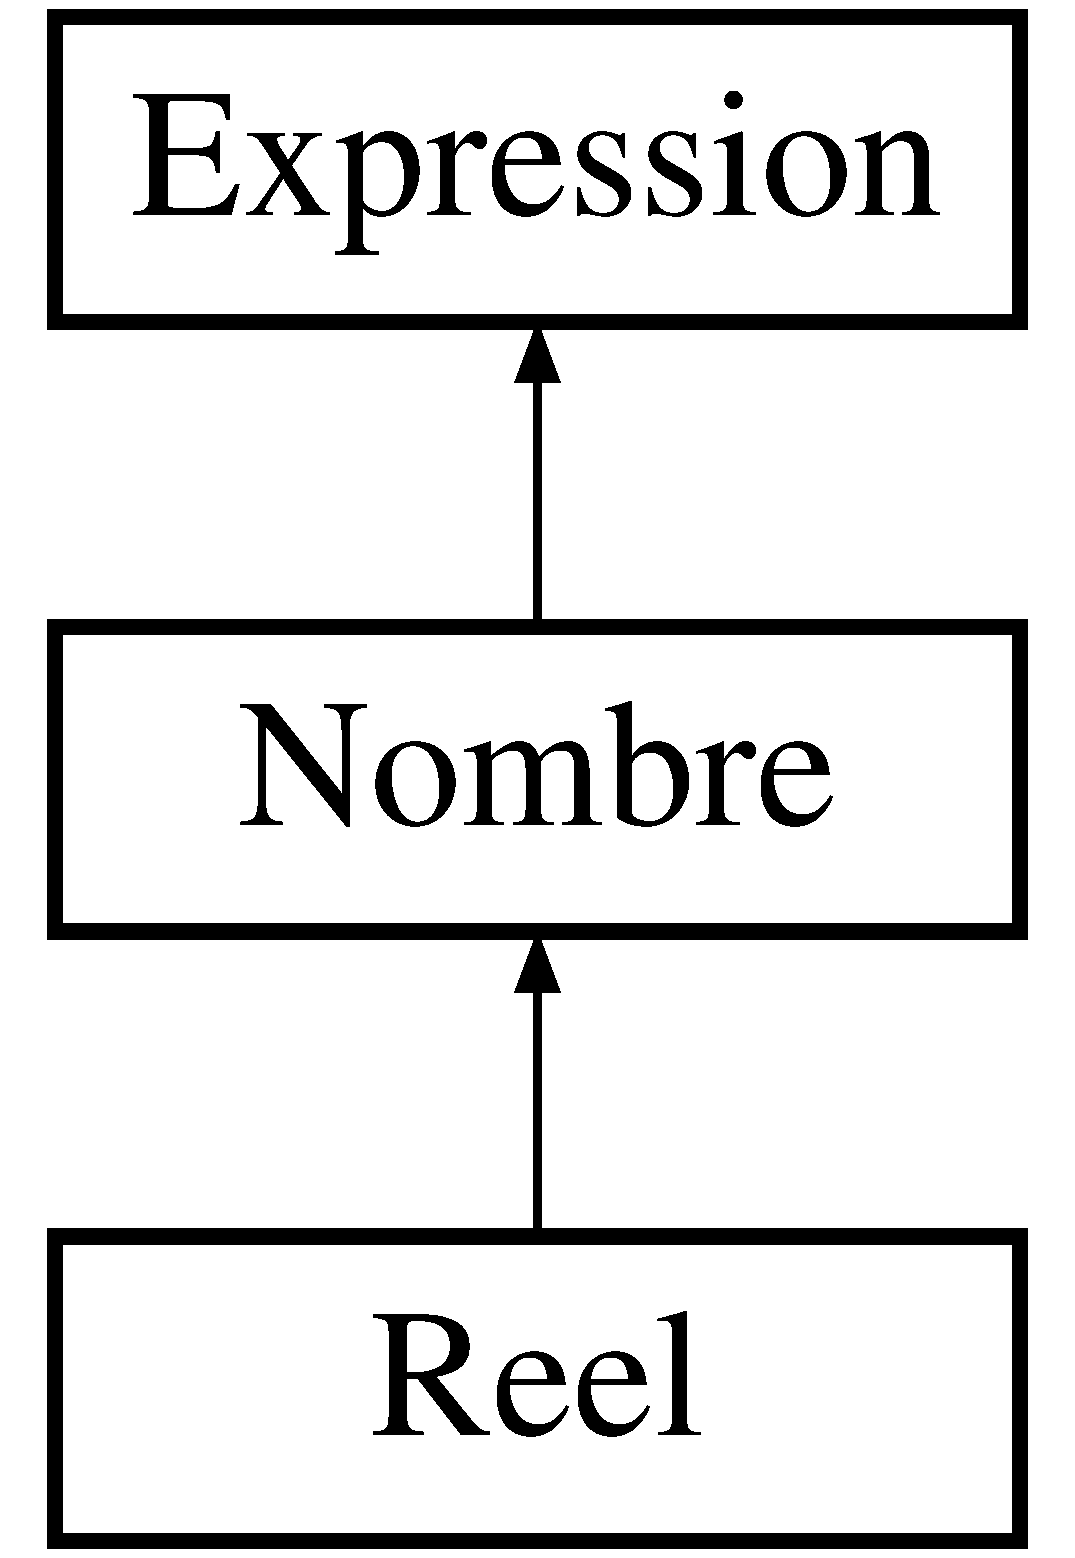
\includegraphics[height=3.000000cm]{class_reel}
\end{center}
\end{figure}
\subsection*{Public Member Functions}
\begin{DoxyCompactItemize}
\item 
{\bf Reel} (double valeur)
\item 
{\bf Reel} ()
\item 
const {\bf Reel} \& {\bf evaluer} () const 
\item 
Q\-String {\bf get\-Propriete} ()
\item 
{\bf Reel} \& {\bf operator=} (const {\bf Reel} \&r)
\item 
{\bf Nombre} \& {\bf operator+} (const {\bf Nombre} \&n)
\item 
{\bf Nombre} \& {\bf operator-\/} (const {\bf Nombre} \&n)
\item 
{\bf Nombre} \& {\bf operator$\ast$} (const {\bf Nombre} \&n)
\item 
{\bf Nombre} \& {\bf operator/} (const {\bf Nombre} \&n)
\end{DoxyCompactItemize}
\subsection*{Additional Inherited Members}


\subsection{Constructor \& Destructor Documentation}
\index{Reel@{Reel}!Reel@{Reel}}
\index{Reel@{Reel}!Reel@{Reel}}
\subsubsection[{Reel}]{\setlength{\rightskip}{0pt plus 5cm}Reel\-::\-Reel (
\begin{DoxyParamCaption}
\item[{double}]{valeur}
\end{DoxyParamCaption}
)}\label{class_reel_a8d0b6879c1f6e546074751bb53cc8190}
\index{Reel@{Reel}!Reel@{Reel}}
\index{Reel@{Reel}!Reel@{Reel}}
\subsubsection[{Reel}]{\setlength{\rightskip}{0pt plus 5cm}Reel\-::\-Reel (
\begin{DoxyParamCaption}
{}
\end{DoxyParamCaption}
)\hspace{0.3cm}{\ttfamily [inline]}}\label{class_reel_a3656fa67f060d2808dc07f337030b537}


\subsection{Member Function Documentation}
\index{Reel@{Reel}!evaluer@{evaluer}}
\index{evaluer@{evaluer}!Reel@{Reel}}
\subsubsection[{evaluer}]{\setlength{\rightskip}{0pt plus 5cm}const {\bf Reel} \& Reel\-::evaluer (
\begin{DoxyParamCaption}
{}
\end{DoxyParamCaption}
) const\hspace{0.3cm}{\ttfamily [virtual]}}\label{class_reel_a880146cec8912d8e959baf46b2d2073b}


Implements {\bf Expression} \doxyref{}{p.}{class_expression_a883dfec27c4579cdd4749ce437d4925e}.

\index{Reel@{Reel}!get\-Propriete@{get\-Propriete}}
\index{get\-Propriete@{get\-Propriete}!Reel@{Reel}}
\subsubsection[{get\-Propriete}]{\setlength{\rightskip}{0pt plus 5cm}Q\-String Reel\-::get\-Propriete (
\begin{DoxyParamCaption}
{}
\end{DoxyParamCaption}
)\hspace{0.3cm}{\ttfamily [inline]}, {\ttfamily [virtual]}}\label{class_reel_ae9cc37231ca8ae433989952ed63e1c98}


Implements {\bf Expression} \doxyref{}{p.}{class_expression_a5c2940c8ca5195f5b9a51234c936e48c}.

\index{Reel@{Reel}!operator$\ast$@{operator$\ast$}}
\index{operator$\ast$@{operator$\ast$}!Reel@{Reel}}
\subsubsection[{operator$\ast$}]{\setlength{\rightskip}{0pt plus 5cm}{\bf Nombre} \& Reel\-::operator$\ast$ (
\begin{DoxyParamCaption}
\item[{const {\bf Nombre} \&}]{n}
\end{DoxyParamCaption}
)\hspace{0.3cm}{\ttfamily [virtual]}}\label{class_reel_a4937d8ec303a13148b9e446d463fec70}


Implements {\bf Nombre} \doxyref{}{p.}{class_nombre_ad249cd1678294bd419da8586ac9fbaa7}.

\index{Reel@{Reel}!operator+@{operator+}}
\index{operator+@{operator+}!Reel@{Reel}}
\subsubsection[{operator+}]{\setlength{\rightskip}{0pt plus 5cm}{\bf Nombre} \& Reel\-::operator+ (
\begin{DoxyParamCaption}
\item[{const {\bf Nombre} \&}]{n}
\end{DoxyParamCaption}
)\hspace{0.3cm}{\ttfamily [virtual]}}\label{class_reel_a02efe680d4baa8c1ca23e65020141767}


Implements {\bf Nombre} \doxyref{}{p.}{class_nombre_a8672fd34bb479f72a9479c146cb33b48}.

\index{Reel@{Reel}!operator-\/@{operator-\/}}
\index{operator-\/@{operator-\/}!Reel@{Reel}}
\subsubsection[{operator-\/}]{\setlength{\rightskip}{0pt plus 5cm}{\bf Nombre} \& Reel\-::operator-\/ (
\begin{DoxyParamCaption}
\item[{const {\bf Nombre} \&}]{n}
\end{DoxyParamCaption}
)\hspace{0.3cm}{\ttfamily [virtual]}}\label{class_reel_ac6d168e265360da5a89bf89a68908696}


Implements {\bf Nombre} \doxyref{}{p.}{class_nombre_a5a281bdf0efbc2a9b557abb8a58e8530}.

\index{Reel@{Reel}!operator/@{operator/}}
\index{operator/@{operator/}!Reel@{Reel}}
\subsubsection[{operator/}]{\setlength{\rightskip}{0pt plus 5cm}{\bf Nombre} \& Reel\-::operator/ (
\begin{DoxyParamCaption}
\item[{const {\bf Nombre} \&}]{n}
\end{DoxyParamCaption}
)\hspace{0.3cm}{\ttfamily [virtual]}}\label{class_reel_ad5fb3c1583c8213581d06e2aa8e1f6df}


Implements {\bf Nombre} \doxyref{}{p.}{class_nombre_a7b55aa0d106bbb34001161fe6e7b8ebc}.

\index{Reel@{Reel}!operator=@{operator=}}
\index{operator=@{operator=}!Reel@{Reel}}
\subsubsection[{operator=}]{\setlength{\rightskip}{0pt plus 5cm}{\bf Reel} \& Reel\-::operator= (
\begin{DoxyParamCaption}
\item[{const {\bf Reel} \&}]{r}
\end{DoxyParamCaption}
)}\label{class_reel_a2134f7d4e44488eadcb0fb08a005a23b}


The documentation for this class was generated from the following files\-:\begin{DoxyCompactItemize}
\item 
calculatrice/{\bf expression.\-h}\item 
calculatrice/{\bf expression.\-cpp}\end{DoxyCompactItemize}

\section{Ui\-\_\-\-Main\-Window Class Reference}
\label{class_ui___main_window}\index{Ui\-\_\-\-Main\-Window@{Ui\-\_\-\-Main\-Window}}


{\ttfamily \#include $<$ui\-\_\-mainwindow.\-h$>$}

Inheritance diagram for Ui\-\_\-\-Main\-Window\-:\begin{figure}[H]
\begin{center}
\leavevmode
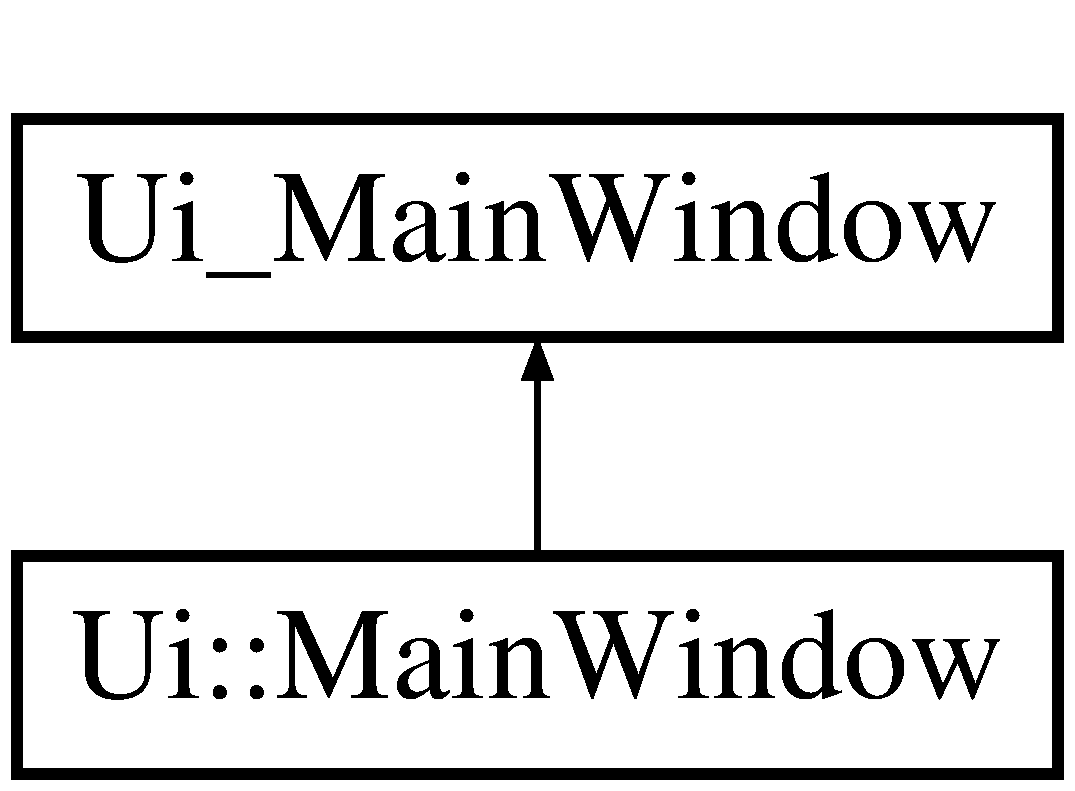
\includegraphics[height=2.000000cm]{class_ui___main_window}
\end{center}
\end{figure}
\subsection*{Public Member Functions}
\begin{DoxyCompactItemize}
\item 
void {\bf setup\-Ui} (Q\-Main\-Window $\ast${\bf Main\-Window})
\item 
void {\bf retranslate\-Ui} (Q\-Main\-Window $\ast${\bf Main\-Window})
\end{DoxyCompactItemize}
\subsection*{Public Attributes}
\begin{DoxyCompactItemize}
\item 
Q\-Action $\ast$ {\bf action}
\item 
Q\-Action $\ast$ {\bf action\-Ouvrir\-\_\-la\-\_\-source}
\item 
Q\-Action $\ast$ {\bf action\-Quit}
\item 
Q\-Widget $\ast$ {\bf central\-Widget}
\item 
Q\-Line\-Edit $\ast$ {\bf line\-\_\-command}
\item 
Q\-Group\-Box $\ast$ {\bf pile}
\item 
Q\-List\-Widget $\ast$ {\bf list\-Widget}
\item 
Q\-Group\-Box $\ast$ {\bf fonction\-\_\-pile}
\item 
Q\-Widget $\ast$ {\bf horizontal\-Layout\-Widget}
\item 
Q\-H\-Box\-Layout $\ast$ {\bf horizontal\-Layout\-\_\-3}
\item 
Q\-Push\-Button $\ast$ {\bf clear}
\item 
Q\-Push\-Button $\ast$ {\bf dup}
\item 
Q\-Push\-Button $\ast$ {\bf drop}
\item 
Q\-Widget $\ast$ {\bf horizontal\-Layout\-Widget\-\_\-2}
\item 
Q\-H\-Box\-Layout $\ast$ {\bf horizontal\-Layout}
\item 
Q\-Push\-Button $\ast$ {\bf mean}
\item 
Q\-Push\-Button $\ast$ {\bf swap}
\item 
Q\-Push\-Button $\ast$ {\bf div}
\item 
Q\-Push\-Button $\ast$ {\bf fact}
\item 
Q\-Push\-Button $\ast$ {\bf sum}
\item 
Q\-Push\-Button $\ast$ {\bf confirmer}
\item 
Q\-Line\-Edit $\ast$ {\bf Result}
\item 
Q\-Label $\ast$ {\bf result}
\item 
Q\-Group\-Box $\ast$ {\bf keyboard}
\item 
Q\-Widget $\ast$ {\bf grid\-Layout\-Widget}
\item 
Q\-Grid\-Layout $\ast$ {\bf grid\-Layout\-\_\-2}
\item 
Q\-Push\-Button $\ast$ {\bf num4}
\item 
Q\-Push\-Button $\ast$ {\bf num5}
\item 
Q\-Push\-Button $\ast$ {\bf num1}
\item 
Q\-Push\-Button $\ast$ {\bf num2}
\item 
Q\-Push\-Button $\ast$ {\bf num3}
\item 
Q\-Push\-Button $\ast$ {\bf num6}
\item 
Q\-Push\-Button $\ast$ {\bf num8}
\item 
Q\-Push\-Button $\ast$ {\bf num7}
\item 
Q\-Push\-Button $\ast$ {\bf num9}
\item 
Q\-Push\-Button $\ast$ {\bf plus}
\item 
Q\-Push\-Button $\ast$ {\bf minus}
\item 
Q\-Push\-Button $\ast$ {\bf multi}
\item 
Q\-Push\-Button $\ast$ {\bf P\-O\-W}
\item 
Q\-Push\-Button $\ast$ {\bf comma}
\item 
Q\-Push\-Button $\ast$ {\bf eval}
\item 
Q\-Push\-Button $\ast$ {\bf entrer}
\item 
Q\-Push\-Button $\ast$ {\bf del}
\item 
Q\-Push\-Button $\ast$ {\bf dollar}
\item 
Q\-Push\-Button $\ast$ {\bf M\-O\-D}
\item 
Q\-Push\-Button $\ast$ {\bf annuler}
\item 
Q\-Push\-Button $\ast$ {\bf retablir}
\item 
Q\-Push\-Button $\ast$ {\bf S\-I\-G\-N}
\item 
Q\-Push\-Button $\ast$ {\bf num0}
\item 
Q\-Push\-Button $\ast$ {\bf espace}
\item 
Q\-Push\-Button $\ast$ {\bf slash}
\item 
Q\-Push\-Button $\ast$ {\bf guillemet}
\item 
Q\-Push\-Button $\ast$ {\bf point}
\item 
Q\-Group\-Box $\ast$ {\bf Fonction\-\_\-unaire}
\item 
Q\-Widget $\ast$ {\bf grid\-Layout\-Widget\-\_\-2}
\item 
Q\-Grid\-Layout $\ast$ {\bf grid\-Layout\-\_\-3}
\item 
Q\-Push\-Button $\ast$ {\bf S\-I\-N}
\item 
Q\-Push\-Button $\ast$ {\bf C\-O\-S}
\item 
Q\-Push\-Button $\ast$ {\bf T\-A\-N}
\item 
Q\-Push\-Button $\ast$ {\bf S\-I\-H\-N}
\item 
Q\-Push\-Button $\ast$ {\bf L\-N}
\item 
Q\-Push\-Button $\ast$ {\bf I\-N\-V}
\item 
Q\-Push\-Button $\ast$ {\bf S\-Q\-R\-T}
\item 
Q\-Push\-Button $\ast$ {\bf S\-Q\-R}
\item 
Q\-Push\-Button $\ast$ {\bf T\-A\-N\-H}
\item 
Q\-Push\-Button $\ast$ {\bf C\-O\-S\-H}
\item 
Q\-Push\-Button $\ast$ {\bf L\-O\-G}
\item 
Q\-Push\-Button $\ast$ {\bf C\-U\-B\-E}
\item 
Q\-Tool\-Bar $\ast$ {\bf main\-Tool\-Bar}
\item 
Q\-Status\-Bar $\ast$ {\bf status\-Bar}
\item 
Q\-Menu\-Bar $\ast$ {\bf menu\-Bar}
\item 
Q\-Menu $\ast$ {\bf menu\-File}
\item 
Q\-Menu $\ast$ {\bf menu\-Help}
\end{DoxyCompactItemize}


\subsection{Member Function Documentation}
\index{Ui\-\_\-\-Main\-Window@{Ui\-\_\-\-Main\-Window}!retranslate\-Ui@{retranslate\-Ui}}
\index{retranslate\-Ui@{retranslate\-Ui}!Ui_MainWindow@{Ui\-\_\-\-Main\-Window}}
\subsubsection[{retranslate\-Ui}]{\setlength{\rightskip}{0pt plus 5cm}void Ui\-\_\-\-Main\-Window\-::retranslate\-Ui (
\begin{DoxyParamCaption}
\item[{Q\-Main\-Window $\ast$}]{Main\-Window}
\end{DoxyParamCaption}
)\hspace{0.3cm}{\ttfamily [inline]}}\label{class_ui___main_window_a097dd160c3534a204904cb374412c618}
\index{Ui\-\_\-\-Main\-Window@{Ui\-\_\-\-Main\-Window}!setup\-Ui@{setup\-Ui}}
\index{setup\-Ui@{setup\-Ui}!Ui_MainWindow@{Ui\-\_\-\-Main\-Window}}
\subsubsection[{setup\-Ui}]{\setlength{\rightskip}{0pt plus 5cm}void Ui\-\_\-\-Main\-Window\-::setup\-Ui (
\begin{DoxyParamCaption}
\item[{Q\-Main\-Window $\ast$}]{Main\-Window}
\end{DoxyParamCaption}
)\hspace{0.3cm}{\ttfamily [inline]}}\label{class_ui___main_window_acf4a0872c4c77d8f43a2ec66ed849b58}


\subsection{Member Data Documentation}
\index{Ui\-\_\-\-Main\-Window@{Ui\-\_\-\-Main\-Window}!action@{action}}
\index{action@{action}!Ui_MainWindow@{Ui\-\_\-\-Main\-Window}}
\subsubsection[{action}]{\setlength{\rightskip}{0pt plus 5cm}Q\-Action$\ast$ Ui\-\_\-\-Main\-Window\-::action}\label{class_ui___main_window_ab2210faf5c81f073c529b01b1dfa0e37}
\index{Ui\-\_\-\-Main\-Window@{Ui\-\_\-\-Main\-Window}!action\-Ouvrir\-\_\-la\-\_\-source@{action\-Ouvrir\-\_\-la\-\_\-source}}
\index{action\-Ouvrir\-\_\-la\-\_\-source@{action\-Ouvrir\-\_\-la\-\_\-source}!Ui_MainWindow@{Ui\-\_\-\-Main\-Window}}
\subsubsection[{action\-Ouvrir\-\_\-la\-\_\-source}]{\setlength{\rightskip}{0pt plus 5cm}Q\-Action$\ast$ Ui\-\_\-\-Main\-Window\-::action\-Ouvrir\-\_\-la\-\_\-source}\label{class_ui___main_window_a00bf613334b256147b030feedd46db21}
\index{Ui\-\_\-\-Main\-Window@{Ui\-\_\-\-Main\-Window}!action\-Quit@{action\-Quit}}
\index{action\-Quit@{action\-Quit}!Ui_MainWindow@{Ui\-\_\-\-Main\-Window}}
\subsubsection[{action\-Quit}]{\setlength{\rightskip}{0pt plus 5cm}Q\-Action$\ast$ Ui\-\_\-\-Main\-Window\-::action\-Quit}\label{class_ui___main_window_a188c243f36a2dbc10e4e2a0ad94273b1}
\index{Ui\-\_\-\-Main\-Window@{Ui\-\_\-\-Main\-Window}!annuler@{annuler}}
\index{annuler@{annuler}!Ui_MainWindow@{Ui\-\_\-\-Main\-Window}}
\subsubsection[{annuler}]{\setlength{\rightskip}{0pt plus 5cm}Q\-Push\-Button$\ast$ Ui\-\_\-\-Main\-Window\-::annuler}\label{class_ui___main_window_afcd80e9772c362343c8b1343fe9cc46f}
\index{Ui\-\_\-\-Main\-Window@{Ui\-\_\-\-Main\-Window}!central\-Widget@{central\-Widget}}
\index{central\-Widget@{central\-Widget}!Ui_MainWindow@{Ui\-\_\-\-Main\-Window}}
\subsubsection[{central\-Widget}]{\setlength{\rightskip}{0pt plus 5cm}Q\-Widget$\ast$ Ui\-\_\-\-Main\-Window\-::central\-Widget}\label{class_ui___main_window_a30075506c2116c3ed4ff25e07ae75f81}
\index{Ui\-\_\-\-Main\-Window@{Ui\-\_\-\-Main\-Window}!clear@{clear}}
\index{clear@{clear}!Ui_MainWindow@{Ui\-\_\-\-Main\-Window}}
\subsubsection[{clear}]{\setlength{\rightskip}{0pt plus 5cm}Q\-Push\-Button$\ast$ Ui\-\_\-\-Main\-Window\-::clear}\label{class_ui___main_window_a77911a9fd66fb7b7ccb5d6194e960d33}
\index{Ui\-\_\-\-Main\-Window@{Ui\-\_\-\-Main\-Window}!comma@{comma}}
\index{comma@{comma}!Ui_MainWindow@{Ui\-\_\-\-Main\-Window}}
\subsubsection[{comma}]{\setlength{\rightskip}{0pt plus 5cm}Q\-Push\-Button$\ast$ Ui\-\_\-\-Main\-Window\-::comma}\label{class_ui___main_window_af841df3624a7820868a97714be5b7110}
\index{Ui\-\_\-\-Main\-Window@{Ui\-\_\-\-Main\-Window}!confirmer@{confirmer}}
\index{confirmer@{confirmer}!Ui_MainWindow@{Ui\-\_\-\-Main\-Window}}
\subsubsection[{confirmer}]{\setlength{\rightskip}{0pt plus 5cm}Q\-Push\-Button$\ast$ Ui\-\_\-\-Main\-Window\-::confirmer}\label{class_ui___main_window_acf394b946d8192e600d87dc1f9a467b4}
\index{Ui\-\_\-\-Main\-Window@{Ui\-\_\-\-Main\-Window}!C\-O\-S@{C\-O\-S}}
\index{C\-O\-S@{C\-O\-S}!Ui_MainWindow@{Ui\-\_\-\-Main\-Window}}
\subsubsection[{C\-O\-S}]{\setlength{\rightskip}{0pt plus 5cm}Q\-Push\-Button$\ast$ Ui\-\_\-\-Main\-Window\-::\-C\-O\-S}\label{class_ui___main_window_acba7c9022bfdd86ca0513771138d1f79}
\index{Ui\-\_\-\-Main\-Window@{Ui\-\_\-\-Main\-Window}!C\-O\-S\-H@{C\-O\-S\-H}}
\index{C\-O\-S\-H@{C\-O\-S\-H}!Ui_MainWindow@{Ui\-\_\-\-Main\-Window}}
\subsubsection[{C\-O\-S\-H}]{\setlength{\rightskip}{0pt plus 5cm}Q\-Push\-Button$\ast$ Ui\-\_\-\-Main\-Window\-::\-C\-O\-S\-H}\label{class_ui___main_window_ab6f966dfd75b5b8164555868f5331ada}
\index{Ui\-\_\-\-Main\-Window@{Ui\-\_\-\-Main\-Window}!C\-U\-B\-E@{C\-U\-B\-E}}
\index{C\-U\-B\-E@{C\-U\-B\-E}!Ui_MainWindow@{Ui\-\_\-\-Main\-Window}}
\subsubsection[{C\-U\-B\-E}]{\setlength{\rightskip}{0pt plus 5cm}Q\-Push\-Button$\ast$ Ui\-\_\-\-Main\-Window\-::\-C\-U\-B\-E}\label{class_ui___main_window_a6808a4c8810a4b54cdcfc0def3b69e4c}
\index{Ui\-\_\-\-Main\-Window@{Ui\-\_\-\-Main\-Window}!del@{del}}
\index{del@{del}!Ui_MainWindow@{Ui\-\_\-\-Main\-Window}}
\subsubsection[{del}]{\setlength{\rightskip}{0pt plus 5cm}Q\-Push\-Button$\ast$ Ui\-\_\-\-Main\-Window\-::del}\label{class_ui___main_window_a147d7b0bc267d1797b13690f66875694}
\index{Ui\-\_\-\-Main\-Window@{Ui\-\_\-\-Main\-Window}!div@{div}}
\index{div@{div}!Ui_MainWindow@{Ui\-\_\-\-Main\-Window}}
\subsubsection[{div}]{\setlength{\rightskip}{0pt plus 5cm}Q\-Push\-Button$\ast$ Ui\-\_\-\-Main\-Window\-::div}\label{class_ui___main_window_ab529ca58e125e2f64435f541216421a3}
\index{Ui\-\_\-\-Main\-Window@{Ui\-\_\-\-Main\-Window}!dollar@{dollar}}
\index{dollar@{dollar}!Ui_MainWindow@{Ui\-\_\-\-Main\-Window}}
\subsubsection[{dollar}]{\setlength{\rightskip}{0pt plus 5cm}Q\-Push\-Button$\ast$ Ui\-\_\-\-Main\-Window\-::dollar}\label{class_ui___main_window_a44e91b3e46daafc1c700ebdc1e99789a}
\index{Ui\-\_\-\-Main\-Window@{Ui\-\_\-\-Main\-Window}!drop@{drop}}
\index{drop@{drop}!Ui_MainWindow@{Ui\-\_\-\-Main\-Window}}
\subsubsection[{drop}]{\setlength{\rightskip}{0pt plus 5cm}Q\-Push\-Button$\ast$ Ui\-\_\-\-Main\-Window\-::drop}\label{class_ui___main_window_a93cc1019ad407d063ab0c95714bbdbd2}
\index{Ui\-\_\-\-Main\-Window@{Ui\-\_\-\-Main\-Window}!dup@{dup}}
\index{dup@{dup}!Ui_MainWindow@{Ui\-\_\-\-Main\-Window}}
\subsubsection[{dup}]{\setlength{\rightskip}{0pt plus 5cm}Q\-Push\-Button$\ast$ Ui\-\_\-\-Main\-Window\-::dup}\label{class_ui___main_window_a06447b27a6b617797f1935c0da8b4fca}
\index{Ui\-\_\-\-Main\-Window@{Ui\-\_\-\-Main\-Window}!entrer@{entrer}}
\index{entrer@{entrer}!Ui_MainWindow@{Ui\-\_\-\-Main\-Window}}
\subsubsection[{entrer}]{\setlength{\rightskip}{0pt plus 5cm}Q\-Push\-Button$\ast$ Ui\-\_\-\-Main\-Window\-::entrer}\label{class_ui___main_window_a4ddf7c4ab13f19e86300500b321b003c}
\index{Ui\-\_\-\-Main\-Window@{Ui\-\_\-\-Main\-Window}!espace@{espace}}
\index{espace@{espace}!Ui_MainWindow@{Ui\-\_\-\-Main\-Window}}
\subsubsection[{espace}]{\setlength{\rightskip}{0pt plus 5cm}Q\-Push\-Button$\ast$ Ui\-\_\-\-Main\-Window\-::espace}\label{class_ui___main_window_a0942b31924b64206cfd7d36d8946fd0a}
\index{Ui\-\_\-\-Main\-Window@{Ui\-\_\-\-Main\-Window}!eval@{eval}}
\index{eval@{eval}!Ui_MainWindow@{Ui\-\_\-\-Main\-Window}}
\subsubsection[{eval}]{\setlength{\rightskip}{0pt plus 5cm}Q\-Push\-Button$\ast$ Ui\-\_\-\-Main\-Window\-::eval}\label{class_ui___main_window_a4a5c262f25072172b908e0addd2b4a68}
\index{Ui\-\_\-\-Main\-Window@{Ui\-\_\-\-Main\-Window}!fact@{fact}}
\index{fact@{fact}!Ui_MainWindow@{Ui\-\_\-\-Main\-Window}}
\subsubsection[{fact}]{\setlength{\rightskip}{0pt plus 5cm}Q\-Push\-Button$\ast$ Ui\-\_\-\-Main\-Window\-::fact}\label{class_ui___main_window_ab9e5d07669e9d976a6f36079cc2c05b7}
\index{Ui\-\_\-\-Main\-Window@{Ui\-\_\-\-Main\-Window}!fonction\-\_\-pile@{fonction\-\_\-pile}}
\index{fonction\-\_\-pile@{fonction\-\_\-pile}!Ui_MainWindow@{Ui\-\_\-\-Main\-Window}}
\subsubsection[{fonction\-\_\-pile}]{\setlength{\rightskip}{0pt plus 5cm}Q\-Group\-Box$\ast$ Ui\-\_\-\-Main\-Window\-::fonction\-\_\-pile}\label{class_ui___main_window_ac4db8ab5d3e9132f5ad2565c1f634897}
\index{Ui\-\_\-\-Main\-Window@{Ui\-\_\-\-Main\-Window}!Fonction\-\_\-unaire@{Fonction\-\_\-unaire}}
\index{Fonction\-\_\-unaire@{Fonction\-\_\-unaire}!Ui_MainWindow@{Ui\-\_\-\-Main\-Window}}
\subsubsection[{Fonction\-\_\-unaire}]{\setlength{\rightskip}{0pt plus 5cm}Q\-Group\-Box$\ast$ Ui\-\_\-\-Main\-Window\-::\-Fonction\-\_\-unaire}\label{class_ui___main_window_ad10fb8b4aeffd877c16684078686ecaf}
\index{Ui\-\_\-\-Main\-Window@{Ui\-\_\-\-Main\-Window}!grid\-Layout\-\_\-2@{grid\-Layout\-\_\-2}}
\index{grid\-Layout\-\_\-2@{grid\-Layout\-\_\-2}!Ui_MainWindow@{Ui\-\_\-\-Main\-Window}}
\subsubsection[{grid\-Layout\-\_\-2}]{\setlength{\rightskip}{0pt plus 5cm}Q\-Grid\-Layout$\ast$ Ui\-\_\-\-Main\-Window\-::grid\-Layout\-\_\-2}\label{class_ui___main_window_a6b2a0c5f7e8ff2a87134908dd770d2d2}
\index{Ui\-\_\-\-Main\-Window@{Ui\-\_\-\-Main\-Window}!grid\-Layout\-\_\-3@{grid\-Layout\-\_\-3}}
\index{grid\-Layout\-\_\-3@{grid\-Layout\-\_\-3}!Ui_MainWindow@{Ui\-\_\-\-Main\-Window}}
\subsubsection[{grid\-Layout\-\_\-3}]{\setlength{\rightskip}{0pt plus 5cm}Q\-Grid\-Layout$\ast$ Ui\-\_\-\-Main\-Window\-::grid\-Layout\-\_\-3}\label{class_ui___main_window_af42ea7d4c2e893181caad21e28166932}
\index{Ui\-\_\-\-Main\-Window@{Ui\-\_\-\-Main\-Window}!grid\-Layout\-Widget@{grid\-Layout\-Widget}}
\index{grid\-Layout\-Widget@{grid\-Layout\-Widget}!Ui_MainWindow@{Ui\-\_\-\-Main\-Window}}
\subsubsection[{grid\-Layout\-Widget}]{\setlength{\rightskip}{0pt plus 5cm}Q\-Widget$\ast$ Ui\-\_\-\-Main\-Window\-::grid\-Layout\-Widget}\label{class_ui___main_window_a08a857edea57a9e53915f22187c06813}
\index{Ui\-\_\-\-Main\-Window@{Ui\-\_\-\-Main\-Window}!grid\-Layout\-Widget\-\_\-2@{grid\-Layout\-Widget\-\_\-2}}
\index{grid\-Layout\-Widget\-\_\-2@{grid\-Layout\-Widget\-\_\-2}!Ui_MainWindow@{Ui\-\_\-\-Main\-Window}}
\subsubsection[{grid\-Layout\-Widget\-\_\-2}]{\setlength{\rightskip}{0pt plus 5cm}Q\-Widget$\ast$ Ui\-\_\-\-Main\-Window\-::grid\-Layout\-Widget\-\_\-2}\label{class_ui___main_window_a9544417b86272b660d07d7e33893a0a5}
\index{Ui\-\_\-\-Main\-Window@{Ui\-\_\-\-Main\-Window}!guillemet@{guillemet}}
\index{guillemet@{guillemet}!Ui_MainWindow@{Ui\-\_\-\-Main\-Window}}
\subsubsection[{guillemet}]{\setlength{\rightskip}{0pt plus 5cm}Q\-Push\-Button$\ast$ Ui\-\_\-\-Main\-Window\-::guillemet}\label{class_ui___main_window_a8317f688a64bc313f9e7747453dc9a11}
\index{Ui\-\_\-\-Main\-Window@{Ui\-\_\-\-Main\-Window}!horizontal\-Layout@{horizontal\-Layout}}
\index{horizontal\-Layout@{horizontal\-Layout}!Ui_MainWindow@{Ui\-\_\-\-Main\-Window}}
\subsubsection[{horizontal\-Layout}]{\setlength{\rightskip}{0pt plus 5cm}Q\-H\-Box\-Layout$\ast$ Ui\-\_\-\-Main\-Window\-::horizontal\-Layout}\label{class_ui___main_window_acd6fdc9ebacc4b25b834162380d75ce8}
\index{Ui\-\_\-\-Main\-Window@{Ui\-\_\-\-Main\-Window}!horizontal\-Layout\-\_\-3@{horizontal\-Layout\-\_\-3}}
\index{horizontal\-Layout\-\_\-3@{horizontal\-Layout\-\_\-3}!Ui_MainWindow@{Ui\-\_\-\-Main\-Window}}
\subsubsection[{horizontal\-Layout\-\_\-3}]{\setlength{\rightskip}{0pt plus 5cm}Q\-H\-Box\-Layout$\ast$ Ui\-\_\-\-Main\-Window\-::horizontal\-Layout\-\_\-3}\label{class_ui___main_window_a03ce63974cc69b067c91bbf285cceca8}
\index{Ui\-\_\-\-Main\-Window@{Ui\-\_\-\-Main\-Window}!horizontal\-Layout\-Widget@{horizontal\-Layout\-Widget}}
\index{horizontal\-Layout\-Widget@{horizontal\-Layout\-Widget}!Ui_MainWindow@{Ui\-\_\-\-Main\-Window}}
\subsubsection[{horizontal\-Layout\-Widget}]{\setlength{\rightskip}{0pt plus 5cm}Q\-Widget$\ast$ Ui\-\_\-\-Main\-Window\-::horizontal\-Layout\-Widget}\label{class_ui___main_window_a9271976c4376de565bfe96c296f4db1e}
\index{Ui\-\_\-\-Main\-Window@{Ui\-\_\-\-Main\-Window}!horizontal\-Layout\-Widget\-\_\-2@{horizontal\-Layout\-Widget\-\_\-2}}
\index{horizontal\-Layout\-Widget\-\_\-2@{horizontal\-Layout\-Widget\-\_\-2}!Ui_MainWindow@{Ui\-\_\-\-Main\-Window}}
\subsubsection[{horizontal\-Layout\-Widget\-\_\-2}]{\setlength{\rightskip}{0pt plus 5cm}Q\-Widget$\ast$ Ui\-\_\-\-Main\-Window\-::horizontal\-Layout\-Widget\-\_\-2}\label{class_ui___main_window_aeb6cecb6a82e31743d3b70d4efb7257b}
\index{Ui\-\_\-\-Main\-Window@{Ui\-\_\-\-Main\-Window}!I\-N\-V@{I\-N\-V}}
\index{I\-N\-V@{I\-N\-V}!Ui_MainWindow@{Ui\-\_\-\-Main\-Window}}
\subsubsection[{I\-N\-V}]{\setlength{\rightskip}{0pt plus 5cm}Q\-Push\-Button$\ast$ Ui\-\_\-\-Main\-Window\-::\-I\-N\-V}\label{class_ui___main_window_a8f44a583b70486ec7584db651ddc3fa6}
\index{Ui\-\_\-\-Main\-Window@{Ui\-\_\-\-Main\-Window}!keyboard@{keyboard}}
\index{keyboard@{keyboard}!Ui_MainWindow@{Ui\-\_\-\-Main\-Window}}
\subsubsection[{keyboard}]{\setlength{\rightskip}{0pt plus 5cm}Q\-Group\-Box$\ast$ Ui\-\_\-\-Main\-Window\-::keyboard}\label{class_ui___main_window_ad218b6687e3151380954bf6bf35e775f}
\index{Ui\-\_\-\-Main\-Window@{Ui\-\_\-\-Main\-Window}!line\-\_\-command@{line\-\_\-command}}
\index{line\-\_\-command@{line\-\_\-command}!Ui_MainWindow@{Ui\-\_\-\-Main\-Window}}
\subsubsection[{line\-\_\-command}]{\setlength{\rightskip}{0pt plus 5cm}Q\-Line\-Edit$\ast$ Ui\-\_\-\-Main\-Window\-::line\-\_\-command}\label{class_ui___main_window_aadfed540d40c3fab343139aa0b4249b4}
\index{Ui\-\_\-\-Main\-Window@{Ui\-\_\-\-Main\-Window}!list\-Widget@{list\-Widget}}
\index{list\-Widget@{list\-Widget}!Ui_MainWindow@{Ui\-\_\-\-Main\-Window}}
\subsubsection[{list\-Widget}]{\setlength{\rightskip}{0pt plus 5cm}Q\-List\-Widget$\ast$ Ui\-\_\-\-Main\-Window\-::list\-Widget}\label{class_ui___main_window_ae647a15635ba8a0e5d5aec475db99d8f}
\index{Ui\-\_\-\-Main\-Window@{Ui\-\_\-\-Main\-Window}!L\-N@{L\-N}}
\index{L\-N@{L\-N}!Ui_MainWindow@{Ui\-\_\-\-Main\-Window}}
\subsubsection[{L\-N}]{\setlength{\rightskip}{0pt plus 5cm}Q\-Push\-Button$\ast$ Ui\-\_\-\-Main\-Window\-::\-L\-N}\label{class_ui___main_window_a62e9dca715645175577d6143bc93fd9f}
\index{Ui\-\_\-\-Main\-Window@{Ui\-\_\-\-Main\-Window}!L\-O\-G@{L\-O\-G}}
\index{L\-O\-G@{L\-O\-G}!Ui_MainWindow@{Ui\-\_\-\-Main\-Window}}
\subsubsection[{L\-O\-G}]{\setlength{\rightskip}{0pt plus 5cm}Q\-Push\-Button$\ast$ Ui\-\_\-\-Main\-Window\-::\-L\-O\-G}\label{class_ui___main_window_a47f156cd397be49d22f6f7fe15b0fde4}
\index{Ui\-\_\-\-Main\-Window@{Ui\-\_\-\-Main\-Window}!main\-Tool\-Bar@{main\-Tool\-Bar}}
\index{main\-Tool\-Bar@{main\-Tool\-Bar}!Ui_MainWindow@{Ui\-\_\-\-Main\-Window}}
\subsubsection[{main\-Tool\-Bar}]{\setlength{\rightskip}{0pt plus 5cm}Q\-Tool\-Bar$\ast$ Ui\-\_\-\-Main\-Window\-::main\-Tool\-Bar}\label{class_ui___main_window_a5172877001c8c7b4e0f6de50421867d1}
\index{Ui\-\_\-\-Main\-Window@{Ui\-\_\-\-Main\-Window}!mean@{mean}}
\index{mean@{mean}!Ui_MainWindow@{Ui\-\_\-\-Main\-Window}}
\subsubsection[{mean}]{\setlength{\rightskip}{0pt plus 5cm}Q\-Push\-Button$\ast$ Ui\-\_\-\-Main\-Window\-::mean}\label{class_ui___main_window_a5fb7e7ae0ff9593f591858fb648053a3}
\index{Ui\-\_\-\-Main\-Window@{Ui\-\_\-\-Main\-Window}!menu\-Bar@{menu\-Bar}}
\index{menu\-Bar@{menu\-Bar}!Ui_MainWindow@{Ui\-\_\-\-Main\-Window}}
\subsubsection[{menu\-Bar}]{\setlength{\rightskip}{0pt plus 5cm}Q\-Menu\-Bar$\ast$ Ui\-\_\-\-Main\-Window\-::menu\-Bar}\label{class_ui___main_window_a2be1c24ec9adfca18e1dcc951931457f}
\index{Ui\-\_\-\-Main\-Window@{Ui\-\_\-\-Main\-Window}!menu\-File@{menu\-File}}
\index{menu\-File@{menu\-File}!Ui_MainWindow@{Ui\-\_\-\-Main\-Window}}
\subsubsection[{menu\-File}]{\setlength{\rightskip}{0pt plus 5cm}Q\-Menu$\ast$ Ui\-\_\-\-Main\-Window\-::menu\-File}\label{class_ui___main_window_a7ba84cb4cdd6a12dc83bf4e100bd8d80}
\index{Ui\-\_\-\-Main\-Window@{Ui\-\_\-\-Main\-Window}!menu\-Help@{menu\-Help}}
\index{menu\-Help@{menu\-Help}!Ui_MainWindow@{Ui\-\_\-\-Main\-Window}}
\subsubsection[{menu\-Help}]{\setlength{\rightskip}{0pt plus 5cm}Q\-Menu$\ast$ Ui\-\_\-\-Main\-Window\-::menu\-Help}\label{class_ui___main_window_ab95dbfbb0550206aeac76db36f491548}
\index{Ui\-\_\-\-Main\-Window@{Ui\-\_\-\-Main\-Window}!minus@{minus}}
\index{minus@{minus}!Ui_MainWindow@{Ui\-\_\-\-Main\-Window}}
\subsubsection[{minus}]{\setlength{\rightskip}{0pt plus 5cm}Q\-Push\-Button$\ast$ Ui\-\_\-\-Main\-Window\-::minus}\label{class_ui___main_window_af9373966419a74f95329806c20e725c6}
\index{Ui\-\_\-\-Main\-Window@{Ui\-\_\-\-Main\-Window}!M\-O\-D@{M\-O\-D}}
\index{M\-O\-D@{M\-O\-D}!Ui_MainWindow@{Ui\-\_\-\-Main\-Window}}
\subsubsection[{M\-O\-D}]{\setlength{\rightskip}{0pt plus 5cm}Q\-Push\-Button$\ast$ Ui\-\_\-\-Main\-Window\-::\-M\-O\-D}\label{class_ui___main_window_a8340a7d6e9beca550e886c360dbc7afb}
\index{Ui\-\_\-\-Main\-Window@{Ui\-\_\-\-Main\-Window}!multi@{multi}}
\index{multi@{multi}!Ui_MainWindow@{Ui\-\_\-\-Main\-Window}}
\subsubsection[{multi}]{\setlength{\rightskip}{0pt plus 5cm}Q\-Push\-Button$\ast$ Ui\-\_\-\-Main\-Window\-::multi}\label{class_ui___main_window_a816519bcd5dbd62552ec153ebb1c0d86}
\index{Ui\-\_\-\-Main\-Window@{Ui\-\_\-\-Main\-Window}!num0@{num0}}
\index{num0@{num0}!Ui_MainWindow@{Ui\-\_\-\-Main\-Window}}
\subsubsection[{num0}]{\setlength{\rightskip}{0pt plus 5cm}Q\-Push\-Button$\ast$ Ui\-\_\-\-Main\-Window\-::num0}\label{class_ui___main_window_ad451216d14bbfb46a45e691f81bd5697}
\index{Ui\-\_\-\-Main\-Window@{Ui\-\_\-\-Main\-Window}!num1@{num1}}
\index{num1@{num1}!Ui_MainWindow@{Ui\-\_\-\-Main\-Window}}
\subsubsection[{num1}]{\setlength{\rightskip}{0pt plus 5cm}Q\-Push\-Button$\ast$ Ui\-\_\-\-Main\-Window\-::num1}\label{class_ui___main_window_a06046b98ba8522d7866ff59b214208d4}
\index{Ui\-\_\-\-Main\-Window@{Ui\-\_\-\-Main\-Window}!num2@{num2}}
\index{num2@{num2}!Ui_MainWindow@{Ui\-\_\-\-Main\-Window}}
\subsubsection[{num2}]{\setlength{\rightskip}{0pt plus 5cm}Q\-Push\-Button$\ast$ Ui\-\_\-\-Main\-Window\-::num2}\label{class_ui___main_window_a42840810d6ba204b30a10316437fbac8}
\index{Ui\-\_\-\-Main\-Window@{Ui\-\_\-\-Main\-Window}!num3@{num3}}
\index{num3@{num3}!Ui_MainWindow@{Ui\-\_\-\-Main\-Window}}
\subsubsection[{num3}]{\setlength{\rightskip}{0pt plus 5cm}Q\-Push\-Button$\ast$ Ui\-\_\-\-Main\-Window\-::num3}\label{class_ui___main_window_a1cba0408985417af8b8f84ecf490f251}
\index{Ui\-\_\-\-Main\-Window@{Ui\-\_\-\-Main\-Window}!num4@{num4}}
\index{num4@{num4}!Ui_MainWindow@{Ui\-\_\-\-Main\-Window}}
\subsubsection[{num4}]{\setlength{\rightskip}{0pt plus 5cm}Q\-Push\-Button$\ast$ Ui\-\_\-\-Main\-Window\-::num4}\label{class_ui___main_window_acec9d7e0484591592b5b5aebe17c4d4c}
\index{Ui\-\_\-\-Main\-Window@{Ui\-\_\-\-Main\-Window}!num5@{num5}}
\index{num5@{num5}!Ui_MainWindow@{Ui\-\_\-\-Main\-Window}}
\subsubsection[{num5}]{\setlength{\rightskip}{0pt plus 5cm}Q\-Push\-Button$\ast$ Ui\-\_\-\-Main\-Window\-::num5}\label{class_ui___main_window_ae2cb73580dc5ebe9ff8bfdeb0be7fa4d}
\index{Ui\-\_\-\-Main\-Window@{Ui\-\_\-\-Main\-Window}!num6@{num6}}
\index{num6@{num6}!Ui_MainWindow@{Ui\-\_\-\-Main\-Window}}
\subsubsection[{num6}]{\setlength{\rightskip}{0pt plus 5cm}Q\-Push\-Button$\ast$ Ui\-\_\-\-Main\-Window\-::num6}\label{class_ui___main_window_a45c01137210fb27261aaa19e878b2771}
\index{Ui\-\_\-\-Main\-Window@{Ui\-\_\-\-Main\-Window}!num7@{num7}}
\index{num7@{num7}!Ui_MainWindow@{Ui\-\_\-\-Main\-Window}}
\subsubsection[{num7}]{\setlength{\rightskip}{0pt plus 5cm}Q\-Push\-Button$\ast$ Ui\-\_\-\-Main\-Window\-::num7}\label{class_ui___main_window_a6b99070e2ed530d98b26f79ce1b5ecdf}
\index{Ui\-\_\-\-Main\-Window@{Ui\-\_\-\-Main\-Window}!num8@{num8}}
\index{num8@{num8}!Ui_MainWindow@{Ui\-\_\-\-Main\-Window}}
\subsubsection[{num8}]{\setlength{\rightskip}{0pt plus 5cm}Q\-Push\-Button$\ast$ Ui\-\_\-\-Main\-Window\-::num8}\label{class_ui___main_window_aeca50b654eb96a8bb380a34405c0e8a6}
\index{Ui\-\_\-\-Main\-Window@{Ui\-\_\-\-Main\-Window}!num9@{num9}}
\index{num9@{num9}!Ui_MainWindow@{Ui\-\_\-\-Main\-Window}}
\subsubsection[{num9}]{\setlength{\rightskip}{0pt plus 5cm}Q\-Push\-Button$\ast$ Ui\-\_\-\-Main\-Window\-::num9}\label{class_ui___main_window_a2a726c1956d35bdc8131b967f8a6d152}
\index{Ui\-\_\-\-Main\-Window@{Ui\-\_\-\-Main\-Window}!pile@{pile}}
\index{pile@{pile}!Ui_MainWindow@{Ui\-\_\-\-Main\-Window}}
\subsubsection[{pile}]{\setlength{\rightskip}{0pt plus 5cm}Q\-Group\-Box$\ast$ Ui\-\_\-\-Main\-Window\-::pile}\label{class_ui___main_window_a8a7d6a07920c7824d62fc7ff85c53309}
\index{Ui\-\_\-\-Main\-Window@{Ui\-\_\-\-Main\-Window}!plus@{plus}}
\index{plus@{plus}!Ui_MainWindow@{Ui\-\_\-\-Main\-Window}}
\subsubsection[{plus}]{\setlength{\rightskip}{0pt plus 5cm}Q\-Push\-Button$\ast$ Ui\-\_\-\-Main\-Window\-::plus}\label{class_ui___main_window_a186af8eccf20a88509bab0284e8b43ba}
\index{Ui\-\_\-\-Main\-Window@{Ui\-\_\-\-Main\-Window}!point@{point}}
\index{point@{point}!Ui_MainWindow@{Ui\-\_\-\-Main\-Window}}
\subsubsection[{point}]{\setlength{\rightskip}{0pt plus 5cm}Q\-Push\-Button$\ast$ Ui\-\_\-\-Main\-Window\-::point}\label{class_ui___main_window_a54b19fcee22b2362d20a10fd55918b14}
\index{Ui\-\_\-\-Main\-Window@{Ui\-\_\-\-Main\-Window}!P\-O\-W@{P\-O\-W}}
\index{P\-O\-W@{P\-O\-W}!Ui_MainWindow@{Ui\-\_\-\-Main\-Window}}
\subsubsection[{P\-O\-W}]{\setlength{\rightskip}{0pt plus 5cm}Q\-Push\-Button$\ast$ Ui\-\_\-\-Main\-Window\-::\-P\-O\-W}\label{class_ui___main_window_a02bdc78125dfec5dfb5653ce0776eeb3}
\index{Ui\-\_\-\-Main\-Window@{Ui\-\_\-\-Main\-Window}!Result@{Result}}
\index{Result@{Result}!Ui_MainWindow@{Ui\-\_\-\-Main\-Window}}
\subsubsection[{Result}]{\setlength{\rightskip}{0pt plus 5cm}Q\-Line\-Edit$\ast$ Ui\-\_\-\-Main\-Window\-::\-Result}\label{class_ui___main_window_a1c4d65a8505459a494e77d01636fd304}
\index{Ui\-\_\-\-Main\-Window@{Ui\-\_\-\-Main\-Window}!result@{result}}
\index{result@{result}!Ui_MainWindow@{Ui\-\_\-\-Main\-Window}}
\subsubsection[{result}]{\setlength{\rightskip}{0pt plus 5cm}Q\-Label$\ast$ Ui\-\_\-\-Main\-Window\-::result}\label{class_ui___main_window_adcaaf1b45961bcecf5315428da79c1be}
\index{Ui\-\_\-\-Main\-Window@{Ui\-\_\-\-Main\-Window}!retablir@{retablir}}
\index{retablir@{retablir}!Ui_MainWindow@{Ui\-\_\-\-Main\-Window}}
\subsubsection[{retablir}]{\setlength{\rightskip}{0pt plus 5cm}Q\-Push\-Button$\ast$ Ui\-\_\-\-Main\-Window\-::retablir}\label{class_ui___main_window_a63ba859b403fa2f74b1e5f3b3f258575}
\index{Ui\-\_\-\-Main\-Window@{Ui\-\_\-\-Main\-Window}!S\-I\-G\-N@{S\-I\-G\-N}}
\index{S\-I\-G\-N@{S\-I\-G\-N}!Ui_MainWindow@{Ui\-\_\-\-Main\-Window}}
\subsubsection[{S\-I\-G\-N}]{\setlength{\rightskip}{0pt plus 5cm}Q\-Push\-Button$\ast$ Ui\-\_\-\-Main\-Window\-::\-S\-I\-G\-N}\label{class_ui___main_window_a5a851ab1cd3ae5dac5d8cf6b6e22e956}
\index{Ui\-\_\-\-Main\-Window@{Ui\-\_\-\-Main\-Window}!S\-I\-H\-N@{S\-I\-H\-N}}
\index{S\-I\-H\-N@{S\-I\-H\-N}!Ui_MainWindow@{Ui\-\_\-\-Main\-Window}}
\subsubsection[{S\-I\-H\-N}]{\setlength{\rightskip}{0pt plus 5cm}Q\-Push\-Button$\ast$ Ui\-\_\-\-Main\-Window\-::\-S\-I\-H\-N}\label{class_ui___main_window_a0265880a275247ffbd5b753285ce7725}
\index{Ui\-\_\-\-Main\-Window@{Ui\-\_\-\-Main\-Window}!S\-I\-N@{S\-I\-N}}
\index{S\-I\-N@{S\-I\-N}!Ui_MainWindow@{Ui\-\_\-\-Main\-Window}}
\subsubsection[{S\-I\-N}]{\setlength{\rightskip}{0pt plus 5cm}Q\-Push\-Button$\ast$ Ui\-\_\-\-Main\-Window\-::\-S\-I\-N}\label{class_ui___main_window_ac1caf33332e6d63e4ec1a9071713493b}
\index{Ui\-\_\-\-Main\-Window@{Ui\-\_\-\-Main\-Window}!slash@{slash}}
\index{slash@{slash}!Ui_MainWindow@{Ui\-\_\-\-Main\-Window}}
\subsubsection[{slash}]{\setlength{\rightskip}{0pt plus 5cm}Q\-Push\-Button$\ast$ Ui\-\_\-\-Main\-Window\-::slash}\label{class_ui___main_window_ac463dd35a3dea778a2670d92493b5c8d}
\index{Ui\-\_\-\-Main\-Window@{Ui\-\_\-\-Main\-Window}!S\-Q\-R@{S\-Q\-R}}
\index{S\-Q\-R@{S\-Q\-R}!Ui_MainWindow@{Ui\-\_\-\-Main\-Window}}
\subsubsection[{S\-Q\-R}]{\setlength{\rightskip}{0pt plus 5cm}Q\-Push\-Button$\ast$ Ui\-\_\-\-Main\-Window\-::\-S\-Q\-R}\label{class_ui___main_window_a6259c463080f8ffe0be91053e874780b}
\index{Ui\-\_\-\-Main\-Window@{Ui\-\_\-\-Main\-Window}!S\-Q\-R\-T@{S\-Q\-R\-T}}
\index{S\-Q\-R\-T@{S\-Q\-R\-T}!Ui_MainWindow@{Ui\-\_\-\-Main\-Window}}
\subsubsection[{S\-Q\-R\-T}]{\setlength{\rightskip}{0pt plus 5cm}Q\-Push\-Button$\ast$ Ui\-\_\-\-Main\-Window\-::\-S\-Q\-R\-T}\label{class_ui___main_window_a6e35980b83db49bf01e02faf128a8ba4}
\index{Ui\-\_\-\-Main\-Window@{Ui\-\_\-\-Main\-Window}!status\-Bar@{status\-Bar}}
\index{status\-Bar@{status\-Bar}!Ui_MainWindow@{Ui\-\_\-\-Main\-Window}}
\subsubsection[{status\-Bar}]{\setlength{\rightskip}{0pt plus 5cm}Q\-Status\-Bar$\ast$ Ui\-\_\-\-Main\-Window\-::status\-Bar}\label{class_ui___main_window_a50fa481337604bcc8bf68de18ab16ecd}
\index{Ui\-\_\-\-Main\-Window@{Ui\-\_\-\-Main\-Window}!sum@{sum}}
\index{sum@{sum}!Ui_MainWindow@{Ui\-\_\-\-Main\-Window}}
\subsubsection[{sum}]{\setlength{\rightskip}{0pt plus 5cm}Q\-Push\-Button$\ast$ Ui\-\_\-\-Main\-Window\-::sum}\label{class_ui___main_window_af99377dc93c5c55a8fcb556539ee0b14}
\index{Ui\-\_\-\-Main\-Window@{Ui\-\_\-\-Main\-Window}!swap@{swap}}
\index{swap@{swap}!Ui_MainWindow@{Ui\-\_\-\-Main\-Window}}
\subsubsection[{swap}]{\setlength{\rightskip}{0pt plus 5cm}Q\-Push\-Button$\ast$ Ui\-\_\-\-Main\-Window\-::swap}\label{class_ui___main_window_a69c4ef9eebd49f9bf048e056f8b3ee84}
\index{Ui\-\_\-\-Main\-Window@{Ui\-\_\-\-Main\-Window}!T\-A\-N@{T\-A\-N}}
\index{T\-A\-N@{T\-A\-N}!Ui_MainWindow@{Ui\-\_\-\-Main\-Window}}
\subsubsection[{T\-A\-N}]{\setlength{\rightskip}{0pt plus 5cm}Q\-Push\-Button$\ast$ Ui\-\_\-\-Main\-Window\-::\-T\-A\-N}\label{class_ui___main_window_a17184ec702aa5040677142c4a143e5f2}
\index{Ui\-\_\-\-Main\-Window@{Ui\-\_\-\-Main\-Window}!T\-A\-N\-H@{T\-A\-N\-H}}
\index{T\-A\-N\-H@{T\-A\-N\-H}!Ui_MainWindow@{Ui\-\_\-\-Main\-Window}}
\subsubsection[{T\-A\-N\-H}]{\setlength{\rightskip}{0pt plus 5cm}Q\-Push\-Button$\ast$ Ui\-\_\-\-Main\-Window\-::\-T\-A\-N\-H}\label{class_ui___main_window_aa0b74bbccda6715c999c78240332fda0}


The documentation for this class was generated from the following file\-:\begin{DoxyCompactItemize}
\item 
calculatrice/{\bf ui\-\_\-mainwindow.\-h}\end{DoxyCompactItemize}

\chapter{File Documentation}
\section{calculatrice/expression.cpp File Reference}
\label{expression_8cpp}\index{calculatrice/expression.\-cpp@{calculatrice/expression.\-cpp}}
{\ttfamily \#include \char`\"{}expression.\-h\char`\"{}}\\*
\subsection*{Functions}
\begin{DoxyCompactItemize}
\item 
{\bf Nombre} \& {\bf power} (const {\bf Nombre} \&n, const {\bf Nombre} \&e)
\item 
{\bf Nombre} \& {\bf modulo} (const {\bf Nombre} \&e1, const {\bf Nombre} \&e2)
\item 
{\bf Nombre} \& {\bf inversion\-Signe} (const {\bf Nombre} \&n)
\item 
{\bf Nombre} \& {\bf tangente\-Hyperbolique} (const {\bf Nombre} \&n)
\item 
{\bf Nombre} \& {\bf cosinus} (const {\bf Nombre} \&n)
\item 
{\bf Nombre} \& {\bf sinus} (const {\bf Nombre} \&n)
\item 
{\bf Nombre} \& {\bf cosinus\-Hyperbolique} (const {\bf Nombre} \&n)
\item 
{\bf Nombre} \& {\bf sinus\-Hyperbolique} (const {\bf Nombre} \&n)
\item 
{\bf Nombre} \& {\bf tangente} (const {\bf Nombre} \&n)
\item 
{\bf Nombre} \& {\bf logarithme} (const {\bf Nombre} \&n)
\item 
{\bf Nombre} \& {\bf inverse} (const {\bf Nombre} \&n)
\item 
{\bf Nombre} \& {\bf racine\-Carree} (const {\bf Nombre} \&n)
\item 
{\bf Nombre} \& {\bf fonction\-Carree} (const {\bf Nombre} \&n)
\item 
{\bf Nombre} \& {\bf fonction\-Cube} (const {\bf Nombre} \&n)
\item 
{\bf Nombre} \& {\bf logarithme10} (const {\bf Nombre} \&n)
\item 
{\bf Nombre} \& {\bf factoriel} (const {\bf Nombre} \&n)
\item 
int {\bf pgcd} (int a, int b)
\item 
void {\bf simplifier} ({\bf Rationnel} \&r)
\end{DoxyCompactItemize}


\subsection{Function Documentation}
\index{expression.\-cpp@{expression.\-cpp}!cosinus@{cosinus}}
\index{cosinus@{cosinus}!expression.cpp@{expression.\-cpp}}
\subsubsection[{cosinus}]{\setlength{\rightskip}{0pt plus 5cm}{\bf Nombre}\& cosinus (
\begin{DoxyParamCaption}
\item[{const {\bf Nombre} \&}]{n}
\end{DoxyParamCaption}
)}\label{expression_8cpp_afc536e6306dfa84571864f0ec756eff8}
\index{expression.\-cpp@{expression.\-cpp}!cosinus\-Hyperbolique@{cosinus\-Hyperbolique}}
\index{cosinus\-Hyperbolique@{cosinus\-Hyperbolique}!expression.cpp@{expression.\-cpp}}
\subsubsection[{cosinus\-Hyperbolique}]{\setlength{\rightskip}{0pt plus 5cm}{\bf Nombre}\& cosinus\-Hyperbolique (
\begin{DoxyParamCaption}
\item[{const {\bf Nombre} \&}]{n}
\end{DoxyParamCaption}
)}\label{expression_8cpp_a29402a4b97f42576e9915bc729d87539}
\index{expression.\-cpp@{expression.\-cpp}!factoriel@{factoriel}}
\index{factoriel@{factoriel}!expression.cpp@{expression.\-cpp}}
\subsubsection[{factoriel}]{\setlength{\rightskip}{0pt plus 5cm}{\bf Nombre}\& factoriel (
\begin{DoxyParamCaption}
\item[{const {\bf Nombre} \&}]{n}
\end{DoxyParamCaption}
)}\label{expression_8cpp_a67191ba03b3d11bbe7b8e868c366b27e}
\index{expression.\-cpp@{expression.\-cpp}!fonction\-Carree@{fonction\-Carree}}
\index{fonction\-Carree@{fonction\-Carree}!expression.cpp@{expression.\-cpp}}
\subsubsection[{fonction\-Carree}]{\setlength{\rightskip}{0pt plus 5cm}{\bf Nombre}\& fonction\-Carree (
\begin{DoxyParamCaption}
\item[{const {\bf Nombre} \&}]{n}
\end{DoxyParamCaption}
)}\label{expression_8cpp_aa4162af2400960d54d14eaa1b5ac184b}
\index{expression.\-cpp@{expression.\-cpp}!fonction\-Cube@{fonction\-Cube}}
\index{fonction\-Cube@{fonction\-Cube}!expression.cpp@{expression.\-cpp}}
\subsubsection[{fonction\-Cube}]{\setlength{\rightskip}{0pt plus 5cm}{\bf Nombre}\& fonction\-Cube (
\begin{DoxyParamCaption}
\item[{const {\bf Nombre} \&}]{n}
\end{DoxyParamCaption}
)}\label{expression_8cpp_a69654740cd07debc18961de5e2e835b9}
\index{expression.\-cpp@{expression.\-cpp}!inverse@{inverse}}
\index{inverse@{inverse}!expression.cpp@{expression.\-cpp}}
\subsubsection[{inverse}]{\setlength{\rightskip}{0pt plus 5cm}{\bf Nombre}\& inverse (
\begin{DoxyParamCaption}
\item[{const {\bf Nombre} \&}]{n}
\end{DoxyParamCaption}
)}\label{expression_8cpp_aeca36b12a1340f0efec5414e6feac404}
\index{expression.\-cpp@{expression.\-cpp}!inversion\-Signe@{inversion\-Signe}}
\index{inversion\-Signe@{inversion\-Signe}!expression.cpp@{expression.\-cpp}}
\subsubsection[{inversion\-Signe}]{\setlength{\rightskip}{0pt plus 5cm}{\bf Nombre}\& inversion\-Signe (
\begin{DoxyParamCaption}
\item[{const {\bf Nombre} \&}]{n}
\end{DoxyParamCaption}
)}\label{expression_8cpp_ab6cf88c562263b87891b60eaa9b4c648}
\index{expression.\-cpp@{expression.\-cpp}!logarithme@{logarithme}}
\index{logarithme@{logarithme}!expression.cpp@{expression.\-cpp}}
\subsubsection[{logarithme}]{\setlength{\rightskip}{0pt plus 5cm}{\bf Nombre}\& logarithme (
\begin{DoxyParamCaption}
\item[{const {\bf Nombre} \&}]{n}
\end{DoxyParamCaption}
)}\label{expression_8cpp_af50aac4e84f8017f77e11fd23a1386b9}
\index{expression.\-cpp@{expression.\-cpp}!logarithme10@{logarithme10}}
\index{logarithme10@{logarithme10}!expression.cpp@{expression.\-cpp}}
\subsubsection[{logarithme10}]{\setlength{\rightskip}{0pt plus 5cm}{\bf Nombre}\& logarithme10 (
\begin{DoxyParamCaption}
\item[{const {\bf Nombre} \&}]{n}
\end{DoxyParamCaption}
)}\label{expression_8cpp_afe6f21c8d0c30ea1a552a3db57718e56}
\index{expression.\-cpp@{expression.\-cpp}!modulo@{modulo}}
\index{modulo@{modulo}!expression.cpp@{expression.\-cpp}}
\subsubsection[{modulo}]{\setlength{\rightskip}{0pt plus 5cm}{\bf Nombre}\& modulo (
\begin{DoxyParamCaption}
\item[{const {\bf Nombre} \&}]{e1, }
\item[{const {\bf Nombre} \&}]{e2}
\end{DoxyParamCaption}
)}\label{expression_8cpp_a1f3bfbfa84f43f80a83a6d53c35b59f1}
\index{expression.\-cpp@{expression.\-cpp}!pgcd@{pgcd}}
\index{pgcd@{pgcd}!expression.cpp@{expression.\-cpp}}
\subsubsection[{pgcd}]{\setlength{\rightskip}{0pt plus 5cm}int pgcd (
\begin{DoxyParamCaption}
\item[{int}]{a, }
\item[{int}]{b}
\end{DoxyParamCaption}
)}\label{expression_8cpp_a7a18f1d2b66a88b6fce563c918d62198}
\index{expression.\-cpp@{expression.\-cpp}!power@{power}}
\index{power@{power}!expression.cpp@{expression.\-cpp}}
\subsubsection[{power}]{\setlength{\rightskip}{0pt plus 5cm}{\bf Nombre}\& power (
\begin{DoxyParamCaption}
\item[{const {\bf Nombre} \&}]{n, }
\item[{const {\bf Nombre} \&}]{e}
\end{DoxyParamCaption}
)}\label{expression_8cpp_ada0b0ab34d10f7b7742ed797d5686ae0}
\index{expression.\-cpp@{expression.\-cpp}!racine\-Carree@{racine\-Carree}}
\index{racine\-Carree@{racine\-Carree}!expression.cpp@{expression.\-cpp}}
\subsubsection[{racine\-Carree}]{\setlength{\rightskip}{0pt plus 5cm}{\bf Nombre}\& racine\-Carree (
\begin{DoxyParamCaption}
\item[{const {\bf Nombre} \&}]{n}
\end{DoxyParamCaption}
)}\label{expression_8cpp_a6c2c0f96e828beb2164a088c7959efd4}
\index{expression.\-cpp@{expression.\-cpp}!simplifier@{simplifier}}
\index{simplifier@{simplifier}!expression.cpp@{expression.\-cpp}}
\subsubsection[{simplifier}]{\setlength{\rightskip}{0pt plus 5cm}void simplifier (
\begin{DoxyParamCaption}
\item[{{\bf Rationnel} \&}]{r}
\end{DoxyParamCaption}
)}\label{expression_8cpp_ac32d1e63b31110fd1605bb0e18b72ea5}
\index{expression.\-cpp@{expression.\-cpp}!sinus@{sinus}}
\index{sinus@{sinus}!expression.cpp@{expression.\-cpp}}
\subsubsection[{sinus}]{\setlength{\rightskip}{0pt plus 5cm}{\bf Nombre}\& sinus (
\begin{DoxyParamCaption}
\item[{const {\bf Nombre} \&}]{n}
\end{DoxyParamCaption}
)}\label{expression_8cpp_a10ce088aff2500b4ae8b6fc05431c82b}
\index{expression.\-cpp@{expression.\-cpp}!sinus\-Hyperbolique@{sinus\-Hyperbolique}}
\index{sinus\-Hyperbolique@{sinus\-Hyperbolique}!expression.cpp@{expression.\-cpp}}
\subsubsection[{sinus\-Hyperbolique}]{\setlength{\rightskip}{0pt plus 5cm}{\bf Nombre}\& sinus\-Hyperbolique (
\begin{DoxyParamCaption}
\item[{const {\bf Nombre} \&}]{n}
\end{DoxyParamCaption}
)}\label{expression_8cpp_af16082a84a9ba5b23fcd25a12194e85d}
\index{expression.\-cpp@{expression.\-cpp}!tangente@{tangente}}
\index{tangente@{tangente}!expression.cpp@{expression.\-cpp}}
\subsubsection[{tangente}]{\setlength{\rightskip}{0pt plus 5cm}{\bf Nombre}\& tangente (
\begin{DoxyParamCaption}
\item[{const {\bf Nombre} \&}]{n}
\end{DoxyParamCaption}
)}\label{expression_8cpp_a22817f65c09f0fdd7166362b54bfa702}
\index{expression.\-cpp@{expression.\-cpp}!tangente\-Hyperbolique@{tangente\-Hyperbolique}}
\index{tangente\-Hyperbolique@{tangente\-Hyperbolique}!expression.cpp@{expression.\-cpp}}
\subsubsection[{tangente\-Hyperbolique}]{\setlength{\rightskip}{0pt plus 5cm}{\bf Nombre}\& tangente\-Hyperbolique (
\begin{DoxyParamCaption}
\item[{const {\bf Nombre} \&}]{n}
\end{DoxyParamCaption}
)}\label{expression_8cpp_adba9b20550f2e9b23d28a5a569c2f259}

\section{calculatrice/expression.h File Reference}
\label{expression_8h}\index{calculatrice/expression.\-h@{calculatrice/expression.\-h}}
{\ttfamily \#include $<$string$>$}\\*
{\ttfamily \#include $<$Q\-String$>$}\\*
{\ttfamily \#include $<$iostream$>$}\\*
{\ttfamily \#include $<$Q\-Reg\-Exp$>$}\\*
{\ttfamily \#include $<$Qdebug$>$}\\*
{\ttfamily \#include $<$math.\-h$>$}\\*
\subsection*{Classes}
\begin{DoxyCompactItemize}
\item 
class {\bf Expression}
\item 
class {\bf Nombre}
\item 
class {\bf Constant}
\item 
class {\bf Complexe}
\item 
class {\bf Reel}
\item 
class {\bf Rationnel}
\item 
class {\bf Entier}
\item 
class {\bf Operation}
\item 
class {\bf Operation\-Binaire}
\item 
class {\bf Operation\-Unaire}
\end{DoxyCompactItemize}
\subsection*{Functions}
\begin{DoxyCompactItemize}
\item 
int {\bf pgcd} (int a, int b)
\item 
void {\bf simplifier} ({\bf Rationnel} \&r)
\item 
{\bf Nombre} \& {\bf power} (const {\bf Nombre} \&n, const {\bf Nombre} \&e)
\item 
{\bf Nombre} \& {\bf modulo} (const {\bf Nombre} \&e1, const {\bf Nombre} \&e2)
\item 
{\bf Nombre} \& {\bf inversion\-Signe} (const {\bf Nombre} \&n)
\item 
{\bf Nombre} \& {\bf sinus} (const {\bf Nombre} \&n)
\item 
{\bf Nombre} \& {\bf cosinus} (const {\bf Nombre} \&n)
\item 
{\bf Nombre} \& {\bf tangente} (const {\bf Nombre} \&n)
\item 
{\bf Nombre} \& {\bf sinus\-Hyperbolique} (const {\bf Nombre} \&n)
\item 
{\bf Nombre} \& {\bf cosinus\-Hyperbolique} (const {\bf Nombre} \&n)
\item 
{\bf Nombre} \& {\bf tangente\-Hyperbolique} (const {\bf Nombre} \&n)
\item 
{\bf Nombre} \& {\bf logarithme} (const {\bf Nombre} \&n)
\item 
{\bf Nombre} \& {\bf inverse} (const {\bf Nombre} \&n)
\item 
{\bf Nombre} \& {\bf racine\-Carree} (const {\bf Nombre} \&n)
\item 
{\bf Nombre} \& {\bf fonction\-Carree} (const {\bf Nombre} \&n)
\item 
{\bf Nombre} \& {\bf logarithme10} (const {\bf Nombre} \&n)
\item 
{\bf Nombre} \& {\bf fonction\-Cube} (const {\bf Nombre} \&n)
\item 
{\bf Nombre} \& {\bf factoriel} (const {\bf Nombre} \&n)
\end{DoxyCompactItemize}


\subsection{Function Documentation}
\index{expression.\-h@{expression.\-h}!cosinus@{cosinus}}
\index{cosinus@{cosinus}!expression.h@{expression.\-h}}
\subsubsection[{cosinus}]{\setlength{\rightskip}{0pt plus 5cm}{\bf Nombre}\& cosinus (
\begin{DoxyParamCaption}
\item[{const {\bf Nombre} \&}]{n}
\end{DoxyParamCaption}
)}\label{expression_8h_afc536e6306dfa84571864f0ec756eff8}
\index{expression.\-h@{expression.\-h}!cosinus\-Hyperbolique@{cosinus\-Hyperbolique}}
\index{cosinus\-Hyperbolique@{cosinus\-Hyperbolique}!expression.h@{expression.\-h}}
\subsubsection[{cosinus\-Hyperbolique}]{\setlength{\rightskip}{0pt plus 5cm}{\bf Nombre}\& cosinus\-Hyperbolique (
\begin{DoxyParamCaption}
\item[{const {\bf Nombre} \&}]{n}
\end{DoxyParamCaption}
)}\label{expression_8h_a29402a4b97f42576e9915bc729d87539}
\index{expression.\-h@{expression.\-h}!factoriel@{factoriel}}
\index{factoriel@{factoriel}!expression.h@{expression.\-h}}
\subsubsection[{factoriel}]{\setlength{\rightskip}{0pt plus 5cm}{\bf Nombre}\& factoriel (
\begin{DoxyParamCaption}
\item[{const {\bf Nombre} \&}]{n}
\end{DoxyParamCaption}
)}\label{expression_8h_a67191ba03b3d11bbe7b8e868c366b27e}
\index{expression.\-h@{expression.\-h}!fonction\-Carree@{fonction\-Carree}}
\index{fonction\-Carree@{fonction\-Carree}!expression.h@{expression.\-h}}
\subsubsection[{fonction\-Carree}]{\setlength{\rightskip}{0pt plus 5cm}{\bf Nombre}\& fonction\-Carree (
\begin{DoxyParamCaption}
\item[{const {\bf Nombre} \&}]{n}
\end{DoxyParamCaption}
)}\label{expression_8h_aa4162af2400960d54d14eaa1b5ac184b}
\index{expression.\-h@{expression.\-h}!fonction\-Cube@{fonction\-Cube}}
\index{fonction\-Cube@{fonction\-Cube}!expression.h@{expression.\-h}}
\subsubsection[{fonction\-Cube}]{\setlength{\rightskip}{0pt plus 5cm}{\bf Nombre}\& fonction\-Cube (
\begin{DoxyParamCaption}
\item[{const {\bf Nombre} \&}]{n}
\end{DoxyParamCaption}
)}\label{expression_8h_a69654740cd07debc18961de5e2e835b9}
\index{expression.\-h@{expression.\-h}!inverse@{inverse}}
\index{inverse@{inverse}!expression.h@{expression.\-h}}
\subsubsection[{inverse}]{\setlength{\rightskip}{0pt plus 5cm}{\bf Nombre}\& inverse (
\begin{DoxyParamCaption}
\item[{const {\bf Nombre} \&}]{n}
\end{DoxyParamCaption}
)}\label{expression_8h_aeca36b12a1340f0efec5414e6feac404}
\index{expression.\-h@{expression.\-h}!inversion\-Signe@{inversion\-Signe}}
\index{inversion\-Signe@{inversion\-Signe}!expression.h@{expression.\-h}}
\subsubsection[{inversion\-Signe}]{\setlength{\rightskip}{0pt plus 5cm}{\bf Nombre}\& inversion\-Signe (
\begin{DoxyParamCaption}
\item[{const {\bf Nombre} \&}]{n}
\end{DoxyParamCaption}
)}\label{expression_8h_ab6cf88c562263b87891b60eaa9b4c648}
\index{expression.\-h@{expression.\-h}!logarithme@{logarithme}}
\index{logarithme@{logarithme}!expression.h@{expression.\-h}}
\subsubsection[{logarithme}]{\setlength{\rightskip}{0pt plus 5cm}{\bf Nombre}\& logarithme (
\begin{DoxyParamCaption}
\item[{const {\bf Nombre} \&}]{n}
\end{DoxyParamCaption}
)}\label{expression_8h_af50aac4e84f8017f77e11fd23a1386b9}
\index{expression.\-h@{expression.\-h}!logarithme10@{logarithme10}}
\index{logarithme10@{logarithme10}!expression.h@{expression.\-h}}
\subsubsection[{logarithme10}]{\setlength{\rightskip}{0pt plus 5cm}{\bf Nombre}\& logarithme10 (
\begin{DoxyParamCaption}
\item[{const {\bf Nombre} \&}]{n}
\end{DoxyParamCaption}
)}\label{expression_8h_afe6f21c8d0c30ea1a552a3db57718e56}
\index{expression.\-h@{expression.\-h}!modulo@{modulo}}
\index{modulo@{modulo}!expression.h@{expression.\-h}}
\subsubsection[{modulo}]{\setlength{\rightskip}{0pt plus 5cm}{\bf Nombre}\& modulo (
\begin{DoxyParamCaption}
\item[{const {\bf Nombre} \&}]{e1, }
\item[{const {\bf Nombre} \&}]{e2}
\end{DoxyParamCaption}
)}\label{expression_8h_a1f3bfbfa84f43f80a83a6d53c35b59f1}
\index{expression.\-h@{expression.\-h}!pgcd@{pgcd}}
\index{pgcd@{pgcd}!expression.h@{expression.\-h}}
\subsubsection[{pgcd}]{\setlength{\rightskip}{0pt plus 5cm}int pgcd (
\begin{DoxyParamCaption}
\item[{int}]{a, }
\item[{int}]{b}
\end{DoxyParamCaption}
)}\label{expression_8h_a7a18f1d2b66a88b6fce563c918d62198}
\index{expression.\-h@{expression.\-h}!power@{power}}
\index{power@{power}!expression.h@{expression.\-h}}
\subsubsection[{power}]{\setlength{\rightskip}{0pt plus 5cm}{\bf Nombre}\& power (
\begin{DoxyParamCaption}
\item[{const {\bf Nombre} \&}]{n, }
\item[{const {\bf Nombre} \&}]{e}
\end{DoxyParamCaption}
)}\label{expression_8h_ada0b0ab34d10f7b7742ed797d5686ae0}
\index{expression.\-h@{expression.\-h}!racine\-Carree@{racine\-Carree}}
\index{racine\-Carree@{racine\-Carree}!expression.h@{expression.\-h}}
\subsubsection[{racine\-Carree}]{\setlength{\rightskip}{0pt plus 5cm}{\bf Nombre}\& racine\-Carree (
\begin{DoxyParamCaption}
\item[{const {\bf Nombre} \&}]{n}
\end{DoxyParamCaption}
)}\label{expression_8h_a6c2c0f96e828beb2164a088c7959efd4}
\index{expression.\-h@{expression.\-h}!simplifier@{simplifier}}
\index{simplifier@{simplifier}!expression.h@{expression.\-h}}
\subsubsection[{simplifier}]{\setlength{\rightskip}{0pt plus 5cm}void simplifier (
\begin{DoxyParamCaption}
\item[{{\bf Rationnel} \&}]{r}
\end{DoxyParamCaption}
)}\label{expression_8h_ac32d1e63b31110fd1605bb0e18b72ea5}
\index{expression.\-h@{expression.\-h}!sinus@{sinus}}
\index{sinus@{sinus}!expression.h@{expression.\-h}}
\subsubsection[{sinus}]{\setlength{\rightskip}{0pt plus 5cm}{\bf Nombre}\& sinus (
\begin{DoxyParamCaption}
\item[{const {\bf Nombre} \&}]{n}
\end{DoxyParamCaption}
)}\label{expression_8h_a10ce088aff2500b4ae8b6fc05431c82b}
\index{expression.\-h@{expression.\-h}!sinus\-Hyperbolique@{sinus\-Hyperbolique}}
\index{sinus\-Hyperbolique@{sinus\-Hyperbolique}!expression.h@{expression.\-h}}
\subsubsection[{sinus\-Hyperbolique}]{\setlength{\rightskip}{0pt plus 5cm}{\bf Nombre}\& sinus\-Hyperbolique (
\begin{DoxyParamCaption}
\item[{const {\bf Nombre} \&}]{n}
\end{DoxyParamCaption}
)}\label{expression_8h_af16082a84a9ba5b23fcd25a12194e85d}
\index{expression.\-h@{expression.\-h}!tangente@{tangente}}
\index{tangente@{tangente}!expression.h@{expression.\-h}}
\subsubsection[{tangente}]{\setlength{\rightskip}{0pt plus 5cm}{\bf Nombre}\& tangente (
\begin{DoxyParamCaption}
\item[{const {\bf Nombre} \&}]{n}
\end{DoxyParamCaption}
)}\label{expression_8h_a22817f65c09f0fdd7166362b54bfa702}
\index{expression.\-h@{expression.\-h}!tangente\-Hyperbolique@{tangente\-Hyperbolique}}
\index{tangente\-Hyperbolique@{tangente\-Hyperbolique}!expression.h@{expression.\-h}}
\subsubsection[{tangente\-Hyperbolique}]{\setlength{\rightskip}{0pt plus 5cm}{\bf Nombre}\& tangente\-Hyperbolique (
\begin{DoxyParamCaption}
\item[{const {\bf Nombre} \&}]{n}
\end{DoxyParamCaption}
)}\label{expression_8h_adba9b20550f2e9b23d28a5a569c2f259}

\section{calculatrice/main.cpp File Reference}
\label{main_8cpp}\index{calculatrice/main.\-cpp@{calculatrice/main.\-cpp}}
{\ttfamily \#include $<$Qt\-Gui/\-Q\-Application$>$}\\*
{\ttfamily \#include \char`\"{}mainwindow.\-h\char`\"{}}\\*
\subsection*{Functions}
\begin{DoxyCompactItemize}
\item 
int {\bf main} (int argc, char $\ast$argv[$\,$])
\end{DoxyCompactItemize}


\subsection{Function Documentation}
\index{main.\-cpp@{main.\-cpp}!main@{main}}
\index{main@{main}!main.cpp@{main.\-cpp}}
\subsubsection[{main}]{\setlength{\rightskip}{0pt plus 5cm}int main (
\begin{DoxyParamCaption}
\item[{int}]{argc, }
\item[{char $\ast$}]{argv[$\,$]}
\end{DoxyParamCaption}
)}\label{main_8cpp_a0ddf1224851353fc92bfbff6f499fa97}

\section{calculatrice/mainwindow.cpp File Reference}
\label{mainwindow_8cpp}\index{calculatrice/mainwindow.\-cpp@{calculatrice/mainwindow.\-cpp}}
{\ttfamily \#include \char`\"{}mainwindow.\-h\char`\"{}}\\*
{\ttfamily \#include \char`\"{}ui\-\_\-mainwindow.\-h\char`\"{}}\\*
{\ttfamily \#include $<$Q\-Push\-Button$>$}\\*

\section{calculatrice/mainwindow.h File Reference}
\label{mainwindow_8h}\index{calculatrice/mainwindow.\-h@{calculatrice/mainwindow.\-h}}
{\ttfamily \#include $<$Q\-Main\-Window$>$}\\*
{\ttfamily \#include $<$Q\-Push\-Button$>$}\\*
{\ttfamily \#include \char`\"{}pile.\-h\char`\"{}}\\*
\subsection*{Classes}
\begin{DoxyCompactItemize}
\item 
class {\bf Main\-Window}
\end{DoxyCompactItemize}
\subsection*{Namespaces}
\begin{DoxyCompactItemize}
\item 
namespace {\bf Ui}
\end{DoxyCompactItemize}

\section{calculatrice/pile.cpp File Reference}
\label{pile_8cpp}\index{calculatrice/pile.\-cpp@{calculatrice/pile.\-cpp}}
{\ttfamily \#include \char`\"{}pile.\-h\char`\"{}}\\*
{\ttfamily \#include $<$Q\-Label$>$}\\*

\section{calculatrice/pile.h File Reference}
\label{pile_8h}\index{calculatrice/pile.\-h@{calculatrice/pile.\-h}}
{\ttfamily \#include $<$Q\-Stack$>$}\\*
{\ttfamily \#include $<$Q\-String$>$}\\*
{\ttfamily \#include $<$Q\-String\-List$>$}\\*
{\ttfamily \#include $<$Q\-Char$>$}\\*
{\ttfamily \#include $<$Q\-Object$>$}\\*
{\ttfamily \#include $<$Q\-Debug$>$}\\*
{\ttfamily \#include $<$Q\-Reg\-Exp$>$}\\*
{\ttfamily \#include \char`\"{}expression.\-h\char`\"{}}\\*
\subsection*{Classes}
\begin{DoxyCompactItemize}
\item 
class {\bf Pile}
\end{DoxyCompactItemize}

\section{calculatrice/ui\-\_\-mainwindow.h File Reference}
\label{ui__mainwindow_8h}\index{calculatrice/ui\-\_\-mainwindow.\-h@{calculatrice/ui\-\_\-mainwindow.\-h}}
{\ttfamily \#include $<$Qt\-Core/\-Q\-Variant$>$}\\*
{\ttfamily \#include $<$Qt\-Gui/\-Q\-Action$>$}\\*
{\ttfamily \#include $<$Qt\-Gui/\-Q\-Application$>$}\\*
{\ttfamily \#include $<$Qt\-Gui/\-Q\-Button\-Group$>$}\\*
{\ttfamily \#include $<$Qt\-Gui/\-Q\-Grid\-Layout$>$}\\*
{\ttfamily \#include $<$Qt\-Gui/\-Q\-Group\-Box$>$}\\*
{\ttfamily \#include $<$Qt\-Gui/\-Q\-H\-Box\-Layout$>$}\\*
{\ttfamily \#include $<$Qt\-Gui/\-Q\-Header\-View$>$}\\*
{\ttfamily \#include $<$Qt\-Gui/\-Q\-Label$>$}\\*
{\ttfamily \#include $<$Qt\-Gui/\-Q\-Line\-Edit$>$}\\*
{\ttfamily \#include $<$Qt\-Gui/\-Q\-List\-Widget$>$}\\*
{\ttfamily \#include $<$Qt\-Gui/\-Q\-Main\-Window$>$}\\*
{\ttfamily \#include $<$Qt\-Gui/\-Q\-Menu$>$}\\*
{\ttfamily \#include $<$Qt\-Gui/\-Q\-Menu\-Bar$>$}\\*
{\ttfamily \#include $<$Qt\-Gui/\-Q\-Push\-Button$>$}\\*
{\ttfamily \#include $<$Qt\-Gui/\-Q\-Status\-Bar$>$}\\*
{\ttfamily \#include $<$Qt\-Gui/\-Q\-Tool\-Bar$>$}\\*
{\ttfamily \#include $<$Qt\-Gui/\-Q\-Widget$>$}\\*
\subsection*{Classes}
\begin{DoxyCompactItemize}
\item 
class {\bf Ui\-\_\-\-Main\-Window}
\item 
class {\bf Ui\-::\-Main\-Window}
\end{DoxyCompactItemize}
\subsection*{Namespaces}
\begin{DoxyCompactItemize}
\item 
namespace {\bf Ui}
\end{DoxyCompactItemize}

\printindex
\end{document}
